\documentclass[conf]{new-aiaa}
%\documentclass[journal]{new-aiaa} for journal papers
\usepackage[utf8]{inputenc}

\usepackage{graphicx}
\usepackage{amsmath}
\usepackage[version=4]{mhchem}
\usepackage{siunitx}
\usepackage{longtable,tabularx}
\setlength\LTleft{0pt} 
\usepackage{multirow}
\usepackage{float}
\usepackage{pgfplots}
\usepackage{tikz}


\title{Optimization of Look-Ahead controller gains for simulation of autonomous vehicle path-tracking}

\author{O. Elsewify\footnote{Master's Student, Mechanical Engineering, 440 Escondido Mall Building 530, Stanford, CA 94305} and A. Mhish\footnote{Master's Student, Mechanical Engineering, 440 Escondido Mall Building 530, Stanford, CA 94305}}
\affil{Stanford University, Stanford, CA, 94305}

\begin{document}

\maketitle

\begin{abstract}
In this paper a design approach is presented for the optimization of the controller gains of a Look-ahead controller for an autonomous vehicle. When implemented, the resulting controller must ensure that the system can follow a fixed trajectory, at a desired speed profile, within a set range of lateral and longitudinal accelerations. The problem is a multi variable optimization problem, with three controller gains as the desired output.
Several optimization approaches are considered and performance of the algorithms are evaluated and compared.
\end{abstract}

\section{Nomenclature}

{\renewcommand\arraystretch{1.0}
\noindent\begin{longtable*}{@{}l @{\quad=\quad} l@{}}
$K_{LA}$ & look-ahead gain \\
$x_{LA}$ & look-ahead distance (m)\\
$K_{long}$& longitudinal gain \\
$\delta$ & steering angle (rad)\\
$F_{x}$ & longitudinal force (N) \\
$\Delta\psi_{ss}$& heading error \\
$e$ & lateral error at CG (m)\\
$\Delta U_x$ & longitudinal vehicle velocity error (m/s)\\
$a_x$ & longitudinal acceleration (m/$s^2$)\\
$a_y$ & lateral acceleration (m/$s^2$)\\
$x$ & design variable \\
$f$ & general function \\
$f_{obj}$   & objective function\\
$c$  & constraints \\
$\alpha$ & step size\\
$\rho$   & initial penalty \\
$\gamma$ & penalty multiplier\\
\end{longtable*}}
$\psi$& radial basis function \\

\section{Introduction}
In the world of controllers, one of the most interesting topics is the topic of path tracking for autonomous vehicles. The objective is to be able to follow a predetermined trajectory and speed profile as closely as possible, using sensors to gather information and a controller and actuators to determine required steering angle and acceleration. There exist several controller types which effectively serve this purpose, each of which undoubtedly requires some degree of tuning and optimisation, there are no off-the-shelf controllers that work for all problems. 

It is the role of control engineers to determine the appropriate parameters (gains) that allow the controller to complete its task effectively. In the past, engineers would be required to generate several control diagram plots including Root-Locus, Nyquist, and Bode, all of which would provide them with a general idea as to what gains should be tested. The typical process for testing and validation of controllers in the physical world can be time consuming and expensive, placing a strong emphasis on the design of an accurate and robust controller before implementation.

With the advent of numerical modeling and simulation, engineers are now able to test and develop their designs in the virtual world at much lower costs. Engineers can iterate through their design parameters hundreds of thousands of times per minute, track improvement in their designs, and finally select the optimal solution to the problem. Furthermore, the computational power of modern machines allow for advanced analysis of large data sets revealing hidden trends in the data that otherwise would go unnoticed.

\section{Vehicle Dynamics and Control Theory}
An ideal controller is designed around two requirements: integrated longitudinal and lateral control, and robustness against noisy inputs \cite{bayuwindra2019look}. The lateral control part of the look-ahead controller takes instantaneous heading error $\Delta\psi$, lateral error $e$, and longitudinal velocity $U_x$ as inputs and returns a steering angle $\delta$ which will point the vehicle towards the path. This relationship can be summarised by the following equation:
\[\Delta\psi_{ss}=\kappa(\frac{maU_x^2}{LC_{{\alpha}r}}-b)\]
\[\delta_{ff}=\frac{K_{LA}x_{LA}}{C_{{\alpha}f}}\Delta\psi_{ss} + \kappa(L+KU_x^2)\]
\[\delta=-\frac{K_{LA}}{C_{{\alpha}f}}(e+x_{LA}\Delta\psi)+\delta_{ff}\]

The second part of the controller involves the control of longitudinal velocity $U_x$, the equivalent of pressing the accelerator pedal.

\begin{figure}[hbt!]
\centering
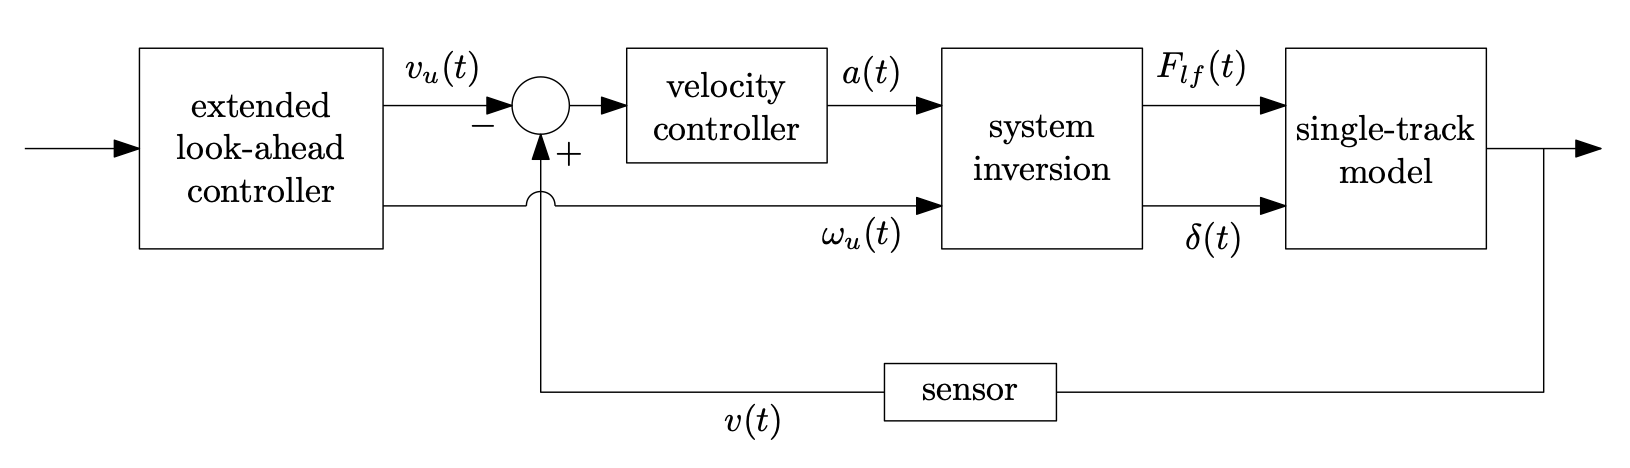
\includegraphics[width=0.75\textwidth]{lookahead_fb}
\caption{Block diagram of the look-ahead controller with integrated longitudinal velocity feedback control\cite{bayuwindra2019look}}
\end{figure}

\section{Optimization Approach}
This paper looks at the iterative design approach for a Look-Ahead controller. The objective of this paper is to develop a robust algorithm that can use an existing data set containing design variables $\textbf{x} \in \mathbb{R}^3$:
\begin{center}
\textbf{x} = [$K_{LA}$    $x_{LA}$  $K_{long}$]
 \end{center}
and their respective simulation results $y($\textbf{x}$)$ $\in \mathbb{R}^4$
 \begin{center}
$y(\textbf{x})$ = [$e$    $\Delta U_{x}$  $a_y$   $a_x$]
 \end{center}
to accurately predict the results for any given $\textbf{x}$. Once this regression model for the function $f$ has been established it is then possible to optimise the for the ideal design variable $x^*$. 
 
The resulting $x^*$ containing the ideal controller gains is then tested in the virtual MATLAB simulation environment and the results are collected and compared against the existing data-set to measure improvement on the existing data samples.

\subsection{Constraints}

There are four main design constraints \textbf{g}(\textbf{x)} imposed on this problem, the first of which is a constraint on the allowable lateral error $e$. The further the vehicle center of gravity is to the left or right of the desired trajectory the larger the error. As such it is best ensure that the lateral error is kept to a minimum, in this problem the allowable lateral error is 20 cm.
\[e\leq0.20\]
The second constraint is on the error in longitudinal velocity tracking $\Delta U_x$. The greater the deviation in the instantaneous velocity from the desired velocity on the speed profile the greater the magnitude of longitudinal velocity error. In this problem the maximum allowable $\Delta U_x$ is 0.75 m/s.
\[\Delta U_x\leq0.75\]
Furthermore, both the maximum lateral and longitudinal accelerations are constrained, such as to reduce the jerkiness motion of the vehicle. A reasonable value of 4 $m/s^2$ is selected for this problem. This constraint is imposed on both the negative (braking) and positive (accelerating) acceleration directions.
\[|a_y|\leq4\]
\[|a_x|\leq4\]
These desired constraints on the acceleration profile are illustrated in Figure \ref{fig:des-acc-profile}
\begin{figure}[htb]
    \begin{center}
        \vspace{-35mm}
        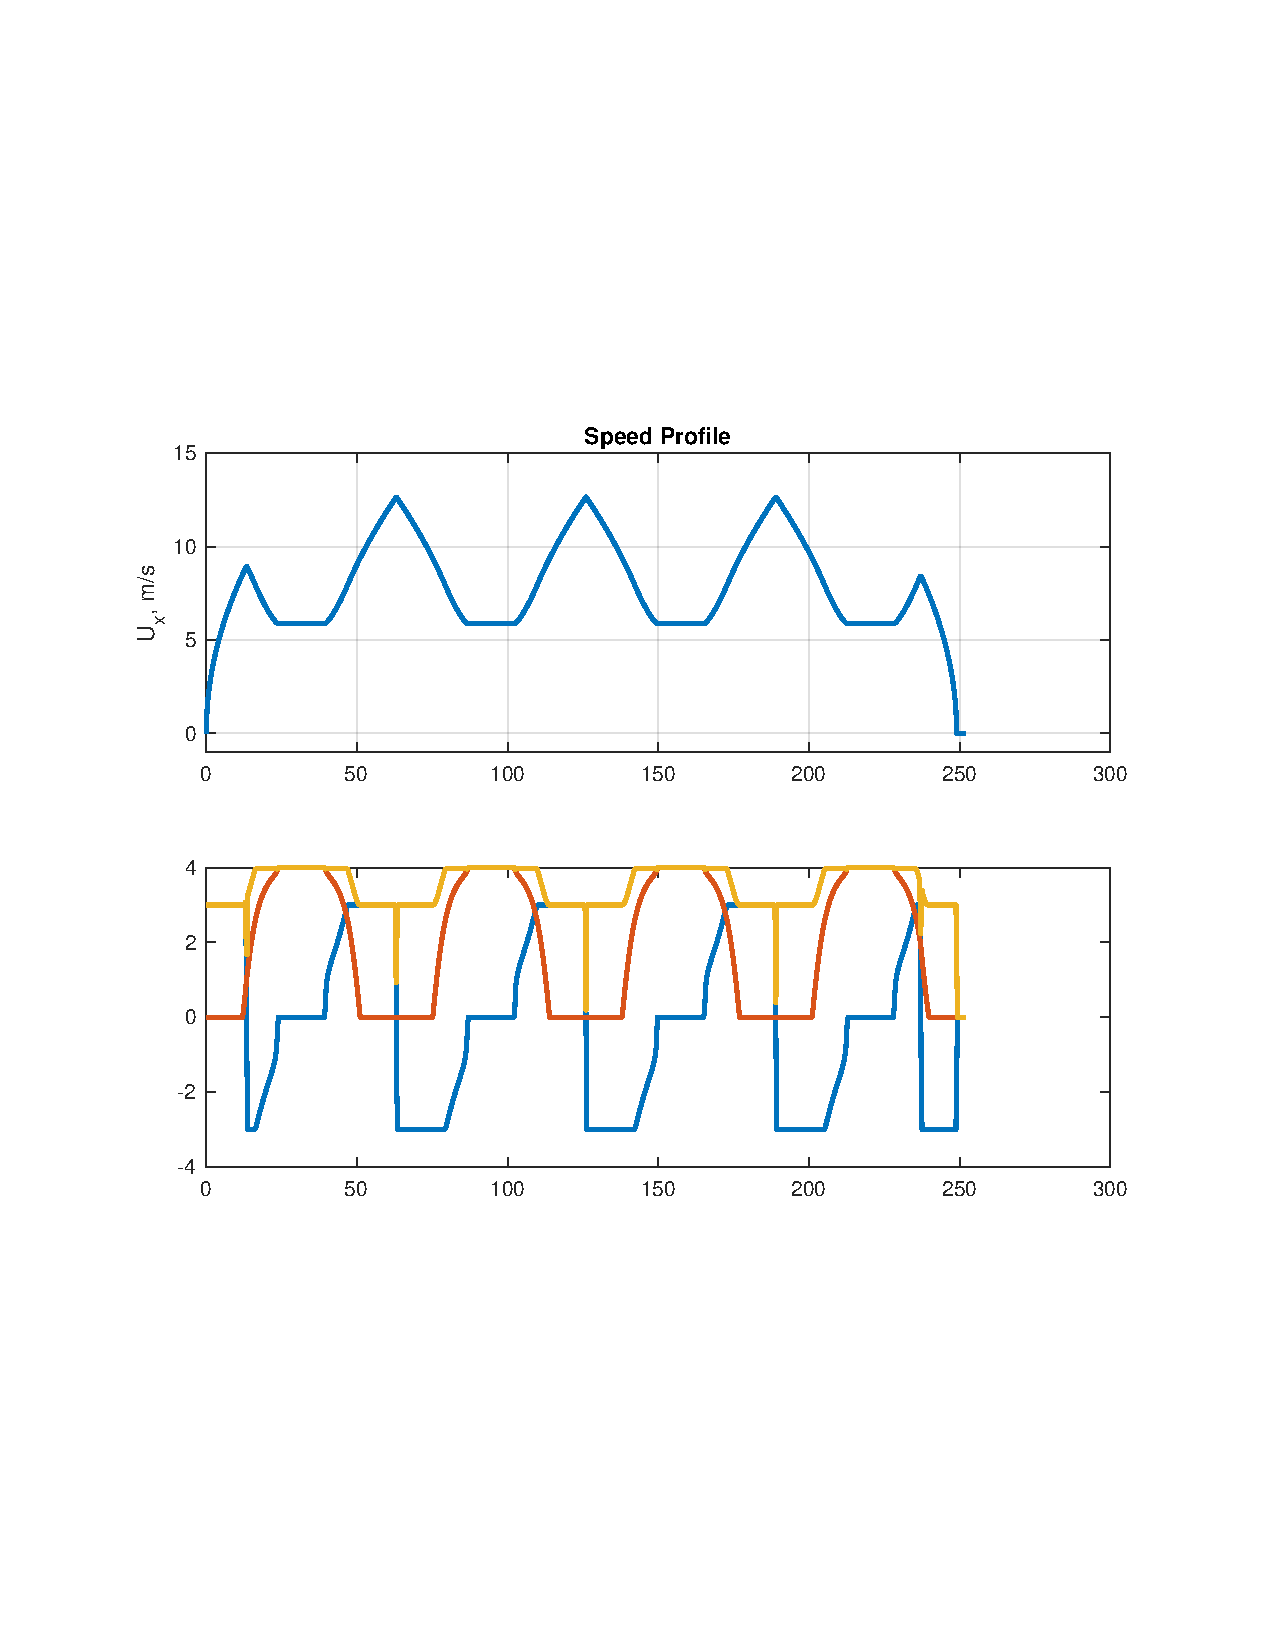
\includegraphics[width =0.6\textwidth]{Desired_Profiles.pdf}
        \vspace{-35mm}
        \caption{Desired speed profile $U_x$ and acceleration profiles for $a_x$ and $a_y$}
        \label{fig:des-acc-profile}
    \end{center}
\end{figure}
\vspace{-10mm}
\subsection{Cost Function}

The cost function designed for this problem is designed with the objective of reducing $e$ and $\Delta U_x$ while minimizing $a_x$ and $a_y$. However, these requirements are not equally weighted, it is more important to ensure the vehicle follows the trajectory than ensuring a comfortable ride. As such as a weighted quadratic penalty function is deployed. For this application a strong emphasis of 10 to 1 is placed on staying within the constraints of lateral and longitudinal velocity error compared to acceleration restriction.
\[\theta = [10, 10, 1, 1]\]
\[p_{qaudratic}(\textbf{x}) = \sum_{i=1}^{4} \theta_i max(g_i(x),0)^2\]
Keeping the constraints in mind, it is still important that the error values and accelerations are minimised, so the objective function includes a sum of the function outputs as well as the penalty outputs.
\[f_{obj}(\textbf{x}) = \sum_{i=1}^{4} f_i(\textbf{x}) + \rho p_{qaudratic}(\textbf{x})\]
The output of this function is a scalar value which maps the effectiveness of a given design variable \textbf{x}. Design variables that reduce this scalar value are deemed more suitable than ones that increase the value.

The optimization problem is formally stated as:
\begin{equation}
\begin{aligned}
\min_{x} \quad & f_{obj}(\textbf{x})\\
\textrm{subject to} \quad &\ e\leq0.20 \\
& \Delta U_{x}\leq0.75 \\
& |a_{y}|\leq4 \\
& |a_{x}|\leq4 \\
\end{aligned}
\end{equation}

\subsection{Function Fitting} % Radial basis functions
In order to fit an accurate model to the data samples at hand, three different function-based models are compared. The goal is to obtain a model that best represents the actual objective function. These types of models are referred to as surrogate models \cite{kochenderfer2019algorithms}.  

For this problem, radial basis functions are used, which are a type of function whose value depends on its distance from the origin. Essentially, the function's response increases or decreases uniformly with distance from a central point c \cite{orr1996introduction}. 

A radial function \[\psi\] can be written as follows:
\[\psi{x,c}=\psi{mod(x-c)}=\psi{r}\]


%ψ(x,c) =ψ(‖x−c‖) =ψ(r)
These types of functions are a favorable choice due to their simplistic design, ease of training, and flexibility.  They also result in very stable models that can represent the data set accurately as a result of their tolerance for input noise \cite{yu2011advantages}.

\subsubsection{Linear Radial Functions}


\subsubsection{Gaussian Radial Functions}


\subsubsection{Inverse Radial Functions}



\subsection{Training and Validation} % Cross-validation vs bootstrap
To make sure that the model fit selected is optimal we need to employ a validation method which returns the generalization error for each surrogate model. The generalization error measures the error of the model on the full design space including points that were not used to train the model. In this paper the expected squared error metric is used to calculate the generalization error:
\[\epsilon_{gen} = \sum_{i=1}^{n} [f(x^{(i)})-y(x^{(i)})]^2\]
with $n$ representing the number of data point in the test set.

\subsubsection{Cross-validation}
The k-fold cross-validation method splits the available data set $X$ in to k randomly partitioned sets of approximately equal size. In each iteration of the method one set is withdrawn for testing and k-1 sets are used to train the model. The withdrawn set is then used to calculate the generalization error of that trained model. By the end of the algorithm k models are trained and k generalization errors are collected. The mean of the generalization is then calculated representing the expected $\epsilon_{gen}$ of the function.

\subsubsection{Bootstrap method}
The limitation of the k-fold cross-validation method is that the testing is done a small fraction of the entire data set increasing the likelihood of bias within the validation process. Bootstrap method addresses this by testing on the entire data set $X$, by training the model on several "synthetic" data sets created by random sampling of the original data set with replacement.

\subsection{Optimization Algorithm} % Hooke-Jeeves vs Cross Entropy
\label{section:Optimization Algorithm}
In this paper two optimization algorithms are examined, the Hook-Jeeves method and the Cross-Entropy method.The results of both algorithms are compared and evaluated to determine the optimal approach/model for the problem.

\subsubsection{Hooke-Jeeves}
The Hooke-Jeeves method is a direct method that takes small steps in each design point coordinate direction. At every iteration the method compares the cost function at anchoring design point \textbf{x} and the cost function at $f(\textbf{x}\pm\alpha \textbf{e}^{(i)})$ for a given step size $\alpha$ in every direction from \textbf{x}, and accepts any improvement found. If no improvements are made then the step size is decreased by a factor of $\gamma$ \cite{kochenderfer2019algorithms}.
However, the performance/suitability of this step size addition and subtraction approach is limited in regards to this problem because the range of magnitudes of each of the design variables is significantly wide. $K_{LA}$ values typically are of the magnitude of $10^3$, $x_LA$ is typically in the range of $10^1$ while $K_{long}$ is typically around $10^{-1}$. This wide range means that a small step size in one variable will  either be too small or too large of a step in another variable. An alternative approach derived from Hooke-Jeeves is deployed in this problem. Instead of using a scalar step change in the design variables, a proportional step change is deployed. Now the objective function is evaluated at $f(\textbf{x}\pm\alpha \textbf{x}^{(i)})$ and compared to the anchor point objective function value. The remaining steps remain the same as Hooke-Jeeves.

\subsubsection{Cross-Entropy}
The cross-entropy algorithm is a stochastic method that incorporates  randomness in design space exploration to help avoid local optima and increase chances of finding a global optimum\cite{rubinstein2004cross}. The points explored are selected using a probability distribution, and at each iteration the distribution is updated to fit a collection of the best samples\cite{kochenderfer2019algorithms}. At each iteration $m$ points are sampled and the best $m_{elite}$ samples are used to fit the proposal distribution for the next iteration. In this paper the the proposal distribution is characterized by a mean vector $\mu$ and a covariance matrix $\Sigma$.

\subsection{Evaluation Approach}
Finally, the optimal solutions that the two methods produce are deployed in the virtual MATLAB simulator and the simulation outputs are compared to the existing data set outputs to evaluate if a new optimal design point was discovered. To make a fair and reproducible comparison the same data set of 31 points is used to train and validate each approach. The following metrics are used for evaluating performance:
\begin{itemize}
\item actual value of cost function using proposed $\textbf{x}^*$
\item deviation of predicted $f(\textbf{x}^*)$ from MATLAB result $y(\textbf{x}^*)$
\item time cost of reaching convergence
\item behaviour of optimisation function convergence
\end{itemize}

\section{Results and Discussion}

\subsection{Evaluation of radial basis functions}
The starting point of the optimization approach involved the determination of an appropriate estimator function $f(\textbf{x})$ that accurately predicts simulation outputs for a given design variable \textbf{x}. Cross-validation and bootstrap were used to train and validate these surrogate models and return a generalisation error. Table \ref{tab:cv_bs_rbf} illustrates these results.
\begin{table}[H]
  \centering
\begin{tabular}{|c|c c c|c c c|}
 \hline
 \cline{2-7} & \multicolumn{6}{|c|}{Mean Generalisation Errors ($10^{-5}$)}\\
 \hline
 \cline{2-7} & \multicolumn{3}{|c|}{Cross-Validation} & \multicolumn{3}{|c|}{Bootstrap}\\
 \hline
  Predictor &Linear & Gaussian & Inverse & Linear & Gaussian & Inverse \\ [0.5ex] 
 \hline
 $e$ & 0.01 & 0.03 & 0.02 & 0.01 & 0.03 & 0.02\\
 \hline
 $\Delta U_x$ & 0.22 & 4.93 & 2.60 & 0.22 & 5.79 & 2.4\\
 \hline
 $a_y$ & 0.55 & 3.60 & 2.72 & 0.52 & 4.08 & 2.45\\
 \hline
 $a_x$ & 0.81 & 1.53 & 1.44 & 0.81 & 1.50 & 1.40\\ [0.5ex] 
 \hline
\end{tabular}
\vspace{2.5mm}
\caption{\label{tab:cv_bs_rbf}Comparison of generalisation errors generated from cross-validation and bootstrap for each radial basis function and predictor function.}
\end{table}
\vspace{-10mm}

% Comment on how linear was actually a poor representation when tested

\subsection{Optimal algorithm selection}
This section compares the two optimisation method mentioned in Section~\ref{section:Optimization Algorithm}. The evolution of each the design point variables (Look-Ahead Gains) is plotted for both methods and the final optimal solution is simulated in the MATLAB environment to return the lateral error $e$ profile and the acceleration profiles $a_x$ and $a_y$.

\subsubsection{Look-ahead Gain}
In both cases the look ahead gain converges to roughly the same value of 2620. However, the path that the two algorithms take to reach this value are very different, the two trajectories are plotted in Figure \ref{fig:k_la_evo}. 
With cross-entropy the look-ahead evolution follows a curved trajectory where each iteration leads to a decrease in the gain value until the value plateaus at which point the algorithm stops. 
On the other hand, the Hooke-Jeeves method only changes the variable when an improvement is found, so the $K_{LA}$ profile remains flat until a large step change improvement is found after roughly 145 iterations that reduce $K_{LA}$ by 0.2\%. The reason it takes such a long time to find an improvement is because the initial percentage step size $\alpha$ is large compared to the other design point variables, this was intentionally done to accommodate the very small magnitude of $K_{long}$. As such the initial percentage step changes are too large to find an improvement in $K_{LA}$. Eventually, once the percentage step change is small enough to find an improvement, an attenuating behaviour is observed. 

\begin{figure}[H]
    \begin{center}
        \vspace{-2.5mm}
        \resizebox{0.6\textwidth}{!}{%% Creator: Matplotlib, PGF backend
%%
%% To include the figure in your LaTeX document, write
%%   \input{<filename>.pgf}
%%
%% Make sure the required packages are loaded in your preamble
%%   \usepackage{pgf}
%%
%% and, on pdftex
%%   \usepackage[utf8]{inputenc}\DeclareUnicodeCharacter{2212}{-}
%%
%% or, on luatex and xetex
%%   \usepackage{unicode-math}
%%
%% Figures using additional raster images can only be included by \input if
%% they are in the same directory as the main LaTeX file. For loading figures
%% from other directories you can use the `import` package
%%   \usepackage{import}
%%
%% and then include the figures with
%%   \import{<path to file>}{<filename>.pgf}
%%
%% Matplotlib used the following preamble
%%
\begingroup%
\makeatletter%
\begin{pgfpicture}%
\pgfpathrectangle{\pgfpointorigin}{\pgfqpoint{6.400000in}{4.800000in}}%
\pgfusepath{use as bounding box, clip}%
\begin{pgfscope}%
\pgfsetbuttcap%
\pgfsetmiterjoin%
\definecolor{currentfill}{rgb}{1.000000,1.000000,1.000000}%
\pgfsetfillcolor{currentfill}%
\pgfsetlinewidth{0.000000pt}%
\definecolor{currentstroke}{rgb}{1.000000,1.000000,1.000000}%
\pgfsetstrokecolor{currentstroke}%
\pgfsetdash{}{0pt}%
\pgfpathmoveto{\pgfqpoint{0.000000in}{0.000000in}}%
\pgfpathlineto{\pgfqpoint{6.400000in}{0.000000in}}%
\pgfpathlineto{\pgfqpoint{6.400000in}{4.800000in}}%
\pgfpathlineto{\pgfqpoint{0.000000in}{4.800000in}}%
\pgfpathclose%
\pgfusepath{fill}%
\end{pgfscope}%
\begin{pgfscope}%
\pgfsetbuttcap%
\pgfsetmiterjoin%
\definecolor{currentfill}{rgb}{1.000000,1.000000,1.000000}%
\pgfsetfillcolor{currentfill}%
\pgfsetlinewidth{0.000000pt}%
\definecolor{currentstroke}{rgb}{0.000000,0.000000,0.000000}%
\pgfsetstrokecolor{currentstroke}%
\pgfsetstrokeopacity{0.000000}%
\pgfsetdash{}{0pt}%
\pgfpathmoveto{\pgfqpoint{0.800000in}{0.528000in}}%
\pgfpathlineto{\pgfqpoint{5.760000in}{0.528000in}}%
\pgfpathlineto{\pgfqpoint{5.760000in}{4.224000in}}%
\pgfpathlineto{\pgfqpoint{0.800000in}{4.224000in}}%
\pgfpathclose%
\pgfusepath{fill}%
\end{pgfscope}%
\begin{pgfscope}%
\pgfsetbuttcap%
\pgfsetroundjoin%
\definecolor{currentfill}{rgb}{0.000000,0.000000,0.000000}%
\pgfsetfillcolor{currentfill}%
\pgfsetlinewidth{0.803000pt}%
\definecolor{currentstroke}{rgb}{0.000000,0.000000,0.000000}%
\pgfsetstrokecolor{currentstroke}%
\pgfsetdash{}{0pt}%
\pgfsys@defobject{currentmarker}{\pgfqpoint{0.000000in}{-0.048611in}}{\pgfqpoint{0.000000in}{0.000000in}}{%
\pgfpathmoveto{\pgfqpoint{0.000000in}{0.000000in}}%
\pgfpathlineto{\pgfqpoint{0.000000in}{-0.048611in}}%
\pgfusepath{stroke,fill}%
}%
\begin{pgfscope}%
\pgfsys@transformshift{1.025455in}{0.528000in}%
\pgfsys@useobject{currentmarker}{}%
\end{pgfscope}%
\end{pgfscope}%
\begin{pgfscope}%
\definecolor{textcolor}{rgb}{0.000000,0.000000,0.000000}%
\pgfsetstrokecolor{textcolor}%
\pgfsetfillcolor{textcolor}%
\pgftext[x=1.025455in,y=0.430778in,,top]{\color{textcolor}\sffamily\fontsize{10.000000}{12.000000}\selectfont 0}%
\end{pgfscope}%
\begin{pgfscope}%
\pgfsetbuttcap%
\pgfsetroundjoin%
\definecolor{currentfill}{rgb}{0.000000,0.000000,0.000000}%
\pgfsetfillcolor{currentfill}%
\pgfsetlinewidth{0.803000pt}%
\definecolor{currentstroke}{rgb}{0.000000,0.000000,0.000000}%
\pgfsetstrokecolor{currentstroke}%
\pgfsetdash{}{0pt}%
\pgfsys@defobject{currentmarker}{\pgfqpoint{0.000000in}{-0.048611in}}{\pgfqpoint{0.000000in}{0.000000in}}{%
\pgfpathmoveto{\pgfqpoint{0.000000in}{0.000000in}}%
\pgfpathlineto{\pgfqpoint{0.000000in}{-0.048611in}}%
\pgfusepath{stroke,fill}%
}%
\begin{pgfscope}%
\pgfsys@transformshift{1.628274in}{0.528000in}%
\pgfsys@useobject{currentmarker}{}%
\end{pgfscope}%
\end{pgfscope}%
\begin{pgfscope}%
\definecolor{textcolor}{rgb}{0.000000,0.000000,0.000000}%
\pgfsetstrokecolor{textcolor}%
\pgfsetfillcolor{textcolor}%
\pgftext[x=1.628274in,y=0.430778in,,top]{\color{textcolor}\sffamily\fontsize{10.000000}{12.000000}\selectfont 25}%
\end{pgfscope}%
\begin{pgfscope}%
\pgfsetbuttcap%
\pgfsetroundjoin%
\definecolor{currentfill}{rgb}{0.000000,0.000000,0.000000}%
\pgfsetfillcolor{currentfill}%
\pgfsetlinewidth{0.803000pt}%
\definecolor{currentstroke}{rgb}{0.000000,0.000000,0.000000}%
\pgfsetstrokecolor{currentstroke}%
\pgfsetdash{}{0pt}%
\pgfsys@defobject{currentmarker}{\pgfqpoint{0.000000in}{-0.048611in}}{\pgfqpoint{0.000000in}{0.000000in}}{%
\pgfpathmoveto{\pgfqpoint{0.000000in}{0.000000in}}%
\pgfpathlineto{\pgfqpoint{0.000000in}{-0.048611in}}%
\pgfusepath{stroke,fill}%
}%
\begin{pgfscope}%
\pgfsys@transformshift{2.231094in}{0.528000in}%
\pgfsys@useobject{currentmarker}{}%
\end{pgfscope}%
\end{pgfscope}%
\begin{pgfscope}%
\definecolor{textcolor}{rgb}{0.000000,0.000000,0.000000}%
\pgfsetstrokecolor{textcolor}%
\pgfsetfillcolor{textcolor}%
\pgftext[x=2.231094in,y=0.430778in,,top]{\color{textcolor}\sffamily\fontsize{10.000000}{12.000000}\selectfont 50}%
\end{pgfscope}%
\begin{pgfscope}%
\pgfsetbuttcap%
\pgfsetroundjoin%
\definecolor{currentfill}{rgb}{0.000000,0.000000,0.000000}%
\pgfsetfillcolor{currentfill}%
\pgfsetlinewidth{0.803000pt}%
\definecolor{currentstroke}{rgb}{0.000000,0.000000,0.000000}%
\pgfsetstrokecolor{currentstroke}%
\pgfsetdash{}{0pt}%
\pgfsys@defobject{currentmarker}{\pgfqpoint{0.000000in}{-0.048611in}}{\pgfqpoint{0.000000in}{0.000000in}}{%
\pgfpathmoveto{\pgfqpoint{0.000000in}{0.000000in}}%
\pgfpathlineto{\pgfqpoint{0.000000in}{-0.048611in}}%
\pgfusepath{stroke,fill}%
}%
\begin{pgfscope}%
\pgfsys@transformshift{2.833913in}{0.528000in}%
\pgfsys@useobject{currentmarker}{}%
\end{pgfscope}%
\end{pgfscope}%
\begin{pgfscope}%
\definecolor{textcolor}{rgb}{0.000000,0.000000,0.000000}%
\pgfsetstrokecolor{textcolor}%
\pgfsetfillcolor{textcolor}%
\pgftext[x=2.833913in,y=0.430778in,,top]{\color{textcolor}\sffamily\fontsize{10.000000}{12.000000}\selectfont 75}%
\end{pgfscope}%
\begin{pgfscope}%
\pgfsetbuttcap%
\pgfsetroundjoin%
\definecolor{currentfill}{rgb}{0.000000,0.000000,0.000000}%
\pgfsetfillcolor{currentfill}%
\pgfsetlinewidth{0.803000pt}%
\definecolor{currentstroke}{rgb}{0.000000,0.000000,0.000000}%
\pgfsetstrokecolor{currentstroke}%
\pgfsetdash{}{0pt}%
\pgfsys@defobject{currentmarker}{\pgfqpoint{0.000000in}{-0.048611in}}{\pgfqpoint{0.000000in}{0.000000in}}{%
\pgfpathmoveto{\pgfqpoint{0.000000in}{0.000000in}}%
\pgfpathlineto{\pgfqpoint{0.000000in}{-0.048611in}}%
\pgfusepath{stroke,fill}%
}%
\begin{pgfscope}%
\pgfsys@transformshift{3.436733in}{0.528000in}%
\pgfsys@useobject{currentmarker}{}%
\end{pgfscope}%
\end{pgfscope}%
\begin{pgfscope}%
\definecolor{textcolor}{rgb}{0.000000,0.000000,0.000000}%
\pgfsetstrokecolor{textcolor}%
\pgfsetfillcolor{textcolor}%
\pgftext[x=3.436733in,y=0.430778in,,top]{\color{textcolor}\sffamily\fontsize{10.000000}{12.000000}\selectfont 100}%
\end{pgfscope}%
\begin{pgfscope}%
\pgfsetbuttcap%
\pgfsetroundjoin%
\definecolor{currentfill}{rgb}{0.000000,0.000000,0.000000}%
\pgfsetfillcolor{currentfill}%
\pgfsetlinewidth{0.803000pt}%
\definecolor{currentstroke}{rgb}{0.000000,0.000000,0.000000}%
\pgfsetstrokecolor{currentstroke}%
\pgfsetdash{}{0pt}%
\pgfsys@defobject{currentmarker}{\pgfqpoint{0.000000in}{-0.048611in}}{\pgfqpoint{0.000000in}{0.000000in}}{%
\pgfpathmoveto{\pgfqpoint{0.000000in}{0.000000in}}%
\pgfpathlineto{\pgfqpoint{0.000000in}{-0.048611in}}%
\pgfusepath{stroke,fill}%
}%
\begin{pgfscope}%
\pgfsys@transformshift{4.039553in}{0.528000in}%
\pgfsys@useobject{currentmarker}{}%
\end{pgfscope}%
\end{pgfscope}%
\begin{pgfscope}%
\definecolor{textcolor}{rgb}{0.000000,0.000000,0.000000}%
\pgfsetstrokecolor{textcolor}%
\pgfsetfillcolor{textcolor}%
\pgftext[x=4.039553in,y=0.430778in,,top]{\color{textcolor}\sffamily\fontsize{10.000000}{12.000000}\selectfont 125}%
\end{pgfscope}%
\begin{pgfscope}%
\pgfsetbuttcap%
\pgfsetroundjoin%
\definecolor{currentfill}{rgb}{0.000000,0.000000,0.000000}%
\pgfsetfillcolor{currentfill}%
\pgfsetlinewidth{0.803000pt}%
\definecolor{currentstroke}{rgb}{0.000000,0.000000,0.000000}%
\pgfsetstrokecolor{currentstroke}%
\pgfsetdash{}{0pt}%
\pgfsys@defobject{currentmarker}{\pgfqpoint{0.000000in}{-0.048611in}}{\pgfqpoint{0.000000in}{0.000000in}}{%
\pgfpathmoveto{\pgfqpoint{0.000000in}{0.000000in}}%
\pgfpathlineto{\pgfqpoint{0.000000in}{-0.048611in}}%
\pgfusepath{stroke,fill}%
}%
\begin{pgfscope}%
\pgfsys@transformshift{4.642372in}{0.528000in}%
\pgfsys@useobject{currentmarker}{}%
\end{pgfscope}%
\end{pgfscope}%
\begin{pgfscope}%
\definecolor{textcolor}{rgb}{0.000000,0.000000,0.000000}%
\pgfsetstrokecolor{textcolor}%
\pgfsetfillcolor{textcolor}%
\pgftext[x=4.642372in,y=0.430778in,,top]{\color{textcolor}\sffamily\fontsize{10.000000}{12.000000}\selectfont 150}%
\end{pgfscope}%
\begin{pgfscope}%
\pgfsetbuttcap%
\pgfsetroundjoin%
\definecolor{currentfill}{rgb}{0.000000,0.000000,0.000000}%
\pgfsetfillcolor{currentfill}%
\pgfsetlinewidth{0.803000pt}%
\definecolor{currentstroke}{rgb}{0.000000,0.000000,0.000000}%
\pgfsetstrokecolor{currentstroke}%
\pgfsetdash{}{0pt}%
\pgfsys@defobject{currentmarker}{\pgfqpoint{0.000000in}{-0.048611in}}{\pgfqpoint{0.000000in}{0.000000in}}{%
\pgfpathmoveto{\pgfqpoint{0.000000in}{0.000000in}}%
\pgfpathlineto{\pgfqpoint{0.000000in}{-0.048611in}}%
\pgfusepath{stroke,fill}%
}%
\begin{pgfscope}%
\pgfsys@transformshift{5.245192in}{0.528000in}%
\pgfsys@useobject{currentmarker}{}%
\end{pgfscope}%
\end{pgfscope}%
\begin{pgfscope}%
\definecolor{textcolor}{rgb}{0.000000,0.000000,0.000000}%
\pgfsetstrokecolor{textcolor}%
\pgfsetfillcolor{textcolor}%
\pgftext[x=5.245192in,y=0.430778in,,top]{\color{textcolor}\sffamily\fontsize{10.000000}{12.000000}\selectfont 175}%
\end{pgfscope}%
\begin{pgfscope}%
\pgfsetbuttcap%
\pgfsetroundjoin%
\definecolor{currentfill}{rgb}{0.000000,0.000000,0.000000}%
\pgfsetfillcolor{currentfill}%
\pgfsetlinewidth{0.803000pt}%
\definecolor{currentstroke}{rgb}{0.000000,0.000000,0.000000}%
\pgfsetstrokecolor{currentstroke}%
\pgfsetdash{}{0pt}%
\pgfsys@defobject{currentmarker}{\pgfqpoint{-0.048611in}{0.000000in}}{\pgfqpoint{-0.000000in}{0.000000in}}{%
\pgfpathmoveto{\pgfqpoint{-0.000000in}{0.000000in}}%
\pgfpathlineto{\pgfqpoint{-0.048611in}{0.000000in}}%
\pgfusepath{stroke,fill}%
}%
\begin{pgfscope}%
\pgfsys@transformshift{0.800000in}{0.715407in}%
\pgfsys@useobject{currentmarker}{}%
\end{pgfscope}%
\end{pgfscope}%
\begin{pgfscope}%
\definecolor{textcolor}{rgb}{0.000000,0.000000,0.000000}%
\pgfsetstrokecolor{textcolor}%
\pgfsetfillcolor{textcolor}%
\pgftext[x=0.424999in, y=0.667182in, left, base]{\color{textcolor}\sffamily\fontsize{10.000000}{12.000000}\selectfont 2619}%
\end{pgfscope}%
\begin{pgfscope}%
\pgfsetbuttcap%
\pgfsetroundjoin%
\definecolor{currentfill}{rgb}{0.000000,0.000000,0.000000}%
\pgfsetfillcolor{currentfill}%
\pgfsetlinewidth{0.803000pt}%
\definecolor{currentstroke}{rgb}{0.000000,0.000000,0.000000}%
\pgfsetstrokecolor{currentstroke}%
\pgfsetdash{}{0pt}%
\pgfsys@defobject{currentmarker}{\pgfqpoint{-0.048611in}{0.000000in}}{\pgfqpoint{-0.000000in}{0.000000in}}{%
\pgfpathmoveto{\pgfqpoint{-0.000000in}{0.000000in}}%
\pgfpathlineto{\pgfqpoint{-0.048611in}{0.000000in}}%
\pgfusepath{stroke,fill}%
}%
\begin{pgfscope}%
\pgfsys@transformshift{0.800000in}{1.227305in}%
\pgfsys@useobject{currentmarker}{}%
\end{pgfscope}%
\end{pgfscope}%
\begin{pgfscope}%
\definecolor{textcolor}{rgb}{0.000000,0.000000,0.000000}%
\pgfsetstrokecolor{textcolor}%
\pgfsetfillcolor{textcolor}%
\pgftext[x=0.424999in, y=1.179079in, left, base]{\color{textcolor}\sffamily\fontsize{10.000000}{12.000000}\selectfont 2620}%
\end{pgfscope}%
\begin{pgfscope}%
\pgfsetbuttcap%
\pgfsetroundjoin%
\definecolor{currentfill}{rgb}{0.000000,0.000000,0.000000}%
\pgfsetfillcolor{currentfill}%
\pgfsetlinewidth{0.803000pt}%
\definecolor{currentstroke}{rgb}{0.000000,0.000000,0.000000}%
\pgfsetstrokecolor{currentstroke}%
\pgfsetdash{}{0pt}%
\pgfsys@defobject{currentmarker}{\pgfqpoint{-0.048611in}{0.000000in}}{\pgfqpoint{-0.000000in}{0.000000in}}{%
\pgfpathmoveto{\pgfqpoint{-0.000000in}{0.000000in}}%
\pgfpathlineto{\pgfqpoint{-0.048611in}{0.000000in}}%
\pgfusepath{stroke,fill}%
}%
\begin{pgfscope}%
\pgfsys@transformshift{0.800000in}{1.739202in}%
\pgfsys@useobject{currentmarker}{}%
\end{pgfscope}%
\end{pgfscope}%
\begin{pgfscope}%
\definecolor{textcolor}{rgb}{0.000000,0.000000,0.000000}%
\pgfsetstrokecolor{textcolor}%
\pgfsetfillcolor{textcolor}%
\pgftext[x=0.424999in, y=1.690977in, left, base]{\color{textcolor}\sffamily\fontsize{10.000000}{12.000000}\selectfont 2621}%
\end{pgfscope}%
\begin{pgfscope}%
\pgfsetbuttcap%
\pgfsetroundjoin%
\definecolor{currentfill}{rgb}{0.000000,0.000000,0.000000}%
\pgfsetfillcolor{currentfill}%
\pgfsetlinewidth{0.803000pt}%
\definecolor{currentstroke}{rgb}{0.000000,0.000000,0.000000}%
\pgfsetstrokecolor{currentstroke}%
\pgfsetdash{}{0pt}%
\pgfsys@defobject{currentmarker}{\pgfqpoint{-0.048611in}{0.000000in}}{\pgfqpoint{-0.000000in}{0.000000in}}{%
\pgfpathmoveto{\pgfqpoint{-0.000000in}{0.000000in}}%
\pgfpathlineto{\pgfqpoint{-0.048611in}{0.000000in}}%
\pgfusepath{stroke,fill}%
}%
\begin{pgfscope}%
\pgfsys@transformshift{0.800000in}{2.251100in}%
\pgfsys@useobject{currentmarker}{}%
\end{pgfscope}%
\end{pgfscope}%
\begin{pgfscope}%
\definecolor{textcolor}{rgb}{0.000000,0.000000,0.000000}%
\pgfsetstrokecolor{textcolor}%
\pgfsetfillcolor{textcolor}%
\pgftext[x=0.424999in, y=2.202874in, left, base]{\color{textcolor}\sffamily\fontsize{10.000000}{12.000000}\selectfont 2622}%
\end{pgfscope}%
\begin{pgfscope}%
\pgfsetbuttcap%
\pgfsetroundjoin%
\definecolor{currentfill}{rgb}{0.000000,0.000000,0.000000}%
\pgfsetfillcolor{currentfill}%
\pgfsetlinewidth{0.803000pt}%
\definecolor{currentstroke}{rgb}{0.000000,0.000000,0.000000}%
\pgfsetstrokecolor{currentstroke}%
\pgfsetdash{}{0pt}%
\pgfsys@defobject{currentmarker}{\pgfqpoint{-0.048611in}{0.000000in}}{\pgfqpoint{-0.000000in}{0.000000in}}{%
\pgfpathmoveto{\pgfqpoint{-0.000000in}{0.000000in}}%
\pgfpathlineto{\pgfqpoint{-0.048611in}{0.000000in}}%
\pgfusepath{stroke,fill}%
}%
\begin{pgfscope}%
\pgfsys@transformshift{0.800000in}{2.762997in}%
\pgfsys@useobject{currentmarker}{}%
\end{pgfscope}%
\end{pgfscope}%
\begin{pgfscope}%
\definecolor{textcolor}{rgb}{0.000000,0.000000,0.000000}%
\pgfsetstrokecolor{textcolor}%
\pgfsetfillcolor{textcolor}%
\pgftext[x=0.424999in, y=2.714772in, left, base]{\color{textcolor}\sffamily\fontsize{10.000000}{12.000000}\selectfont 2623}%
\end{pgfscope}%
\begin{pgfscope}%
\pgfsetbuttcap%
\pgfsetroundjoin%
\definecolor{currentfill}{rgb}{0.000000,0.000000,0.000000}%
\pgfsetfillcolor{currentfill}%
\pgfsetlinewidth{0.803000pt}%
\definecolor{currentstroke}{rgb}{0.000000,0.000000,0.000000}%
\pgfsetstrokecolor{currentstroke}%
\pgfsetdash{}{0pt}%
\pgfsys@defobject{currentmarker}{\pgfqpoint{-0.048611in}{0.000000in}}{\pgfqpoint{-0.000000in}{0.000000in}}{%
\pgfpathmoveto{\pgfqpoint{-0.000000in}{0.000000in}}%
\pgfpathlineto{\pgfqpoint{-0.048611in}{0.000000in}}%
\pgfusepath{stroke,fill}%
}%
\begin{pgfscope}%
\pgfsys@transformshift{0.800000in}{3.274895in}%
\pgfsys@useobject{currentmarker}{}%
\end{pgfscope}%
\end{pgfscope}%
\begin{pgfscope}%
\definecolor{textcolor}{rgb}{0.000000,0.000000,0.000000}%
\pgfsetstrokecolor{textcolor}%
\pgfsetfillcolor{textcolor}%
\pgftext[x=0.424999in, y=3.226669in, left, base]{\color{textcolor}\sffamily\fontsize{10.000000}{12.000000}\selectfont 2624}%
\end{pgfscope}%
\begin{pgfscope}%
\pgfsetbuttcap%
\pgfsetroundjoin%
\definecolor{currentfill}{rgb}{0.000000,0.000000,0.000000}%
\pgfsetfillcolor{currentfill}%
\pgfsetlinewidth{0.803000pt}%
\definecolor{currentstroke}{rgb}{0.000000,0.000000,0.000000}%
\pgfsetstrokecolor{currentstroke}%
\pgfsetdash{}{0pt}%
\pgfsys@defobject{currentmarker}{\pgfqpoint{-0.048611in}{0.000000in}}{\pgfqpoint{-0.000000in}{0.000000in}}{%
\pgfpathmoveto{\pgfqpoint{-0.000000in}{0.000000in}}%
\pgfpathlineto{\pgfqpoint{-0.048611in}{0.000000in}}%
\pgfusepath{stroke,fill}%
}%
\begin{pgfscope}%
\pgfsys@transformshift{0.800000in}{3.786792in}%
\pgfsys@useobject{currentmarker}{}%
\end{pgfscope}%
\end{pgfscope}%
\begin{pgfscope}%
\definecolor{textcolor}{rgb}{0.000000,0.000000,0.000000}%
\pgfsetstrokecolor{textcolor}%
\pgfsetfillcolor{textcolor}%
\pgftext[x=0.424999in, y=3.738567in, left, base]{\color{textcolor}\sffamily\fontsize{10.000000}{12.000000}\selectfont 2625}%
\end{pgfscope}%
\begin{pgfscope}%
\pgfpathrectangle{\pgfqpoint{0.800000in}{0.528000in}}{\pgfqpoint{4.960000in}{3.696000in}}%
\pgfusepath{clip}%
\pgfsetrectcap%
\pgfsetroundjoin%
\pgfsetlinewidth{1.505625pt}%
\definecolor{currentstroke}{rgb}{0.121569,0.466667,0.705882}%
\pgfsetstrokecolor{currentstroke}%
\pgfsetdash{}{0pt}%
\pgfpathmoveto{\pgfqpoint{1.025455in}{3.914943in}}%
\pgfpathlineto{\pgfqpoint{1.049567in}{3.758606in}}%
\pgfpathlineto{\pgfqpoint{1.073680in}{3.720580in}}%
\pgfpathlineto{\pgfqpoint{1.097793in}{3.649272in}}%
\pgfpathlineto{\pgfqpoint{1.121906in}{3.555108in}}%
\pgfpathlineto{\pgfqpoint{1.146018in}{3.533950in}}%
\pgfpathlineto{\pgfqpoint{1.170131in}{3.473748in}}%
\pgfpathlineto{\pgfqpoint{1.194244in}{3.427311in}}%
\pgfpathlineto{\pgfqpoint{1.218357in}{3.387592in}}%
\pgfpathlineto{\pgfqpoint{1.242470in}{3.321072in}}%
\pgfpathlineto{\pgfqpoint{1.266582in}{3.304975in}}%
\pgfpathlineto{\pgfqpoint{1.290695in}{3.296514in}}%
\pgfpathlineto{\pgfqpoint{1.314808in}{3.263088in}}%
\pgfpathlineto{\pgfqpoint{1.338921in}{3.289781in}}%
\pgfpathlineto{\pgfqpoint{1.363034in}{3.257451in}}%
\pgfpathlineto{\pgfqpoint{1.387146in}{3.240423in}}%
\pgfpathlineto{\pgfqpoint{1.411259in}{3.184419in}}%
\pgfpathlineto{\pgfqpoint{1.435372in}{3.199714in}}%
\pgfpathlineto{\pgfqpoint{1.459485in}{3.171127in}}%
\pgfpathlineto{\pgfqpoint{1.483597in}{3.117598in}}%
\pgfpathlineto{\pgfqpoint{1.507710in}{3.147987in}}%
\pgfpathlineto{\pgfqpoint{1.531823in}{3.135492in}}%
\pgfpathlineto{\pgfqpoint{1.555936in}{3.130247in}}%
\pgfpathlineto{\pgfqpoint{1.580049in}{3.092005in}}%
\pgfpathlineto{\pgfqpoint{1.604161in}{3.088488in}}%
\pgfpathlineto{\pgfqpoint{1.628274in}{3.097488in}}%
\pgfpathlineto{\pgfqpoint{1.652387in}{3.059516in}}%
\pgfpathlineto{\pgfqpoint{1.676500in}{3.017415in}}%
\pgfpathlineto{\pgfqpoint{1.700613in}{3.013696in}}%
\pgfpathlineto{\pgfqpoint{1.724725in}{3.003815in}}%
\pgfpathlineto{\pgfqpoint{1.748838in}{2.976279in}}%
\pgfpathlineto{\pgfqpoint{1.772951in}{2.956777in}}%
\pgfpathlineto{\pgfqpoint{1.797064in}{2.934688in}}%
\pgfpathlineto{\pgfqpoint{1.821176in}{2.899343in}}%
\pgfpathlineto{\pgfqpoint{1.845289in}{2.860711in}}%
\pgfpathlineto{\pgfqpoint{1.869402in}{2.903043in}}%
\pgfpathlineto{\pgfqpoint{1.893515in}{2.848545in}}%
\pgfpathlineto{\pgfqpoint{1.917628in}{2.807787in}}%
\pgfpathlineto{\pgfqpoint{1.941740in}{2.768579in}}%
\pgfpathlineto{\pgfqpoint{1.965853in}{2.724076in}}%
\pgfpathlineto{\pgfqpoint{1.989966in}{2.754838in}}%
\pgfpathlineto{\pgfqpoint{2.014079in}{2.759631in}}%
\pgfpathlineto{\pgfqpoint{2.038192in}{2.707662in}}%
\pgfpathlineto{\pgfqpoint{2.062304in}{2.691067in}}%
\pgfpathlineto{\pgfqpoint{2.086417in}{2.709682in}}%
\pgfpathlineto{\pgfqpoint{2.110530in}{2.659913in}}%
\pgfpathlineto{\pgfqpoint{2.134643in}{2.634008in}}%
\pgfpathlineto{\pgfqpoint{2.158755in}{2.645032in}}%
\pgfpathlineto{\pgfqpoint{2.182868in}{2.626013in}}%
\pgfpathlineto{\pgfqpoint{2.206981in}{2.578708in}}%
\pgfpathlineto{\pgfqpoint{2.231094in}{2.550750in}}%
\pgfpathlineto{\pgfqpoint{2.255207in}{2.505305in}}%
\pgfpathlineto{\pgfqpoint{2.279319in}{2.512517in}}%
\pgfpathlineto{\pgfqpoint{2.303432in}{2.518277in}}%
\pgfpathlineto{\pgfqpoint{2.327545in}{2.528408in}}%
\pgfpathlineto{\pgfqpoint{2.351658in}{2.485225in}}%
\pgfpathlineto{\pgfqpoint{2.375771in}{2.486784in}}%
\pgfpathlineto{\pgfqpoint{2.399883in}{2.479519in}}%
\pgfpathlineto{\pgfqpoint{2.423996in}{2.470288in}}%
\pgfpathlineto{\pgfqpoint{2.448109in}{2.437714in}}%
\pgfpathlineto{\pgfqpoint{2.472222in}{2.476263in}}%
\pgfpathlineto{\pgfqpoint{2.496334in}{2.435142in}}%
\pgfpathlineto{\pgfqpoint{2.520447in}{2.423557in}}%
\pgfpathlineto{\pgfqpoint{2.544560in}{2.378745in}}%
\pgfpathlineto{\pgfqpoint{2.568673in}{2.375956in}}%
\pgfpathlineto{\pgfqpoint{2.592786in}{2.321780in}}%
\pgfpathlineto{\pgfqpoint{2.616898in}{2.303264in}}%
\pgfpathlineto{\pgfqpoint{2.641011in}{2.297963in}}%
\pgfpathlineto{\pgfqpoint{2.665124in}{2.271242in}}%
\pgfpathlineto{\pgfqpoint{2.689237in}{2.268077in}}%
\pgfpathlineto{\pgfqpoint{2.713350in}{2.272224in}}%
\pgfpathlineto{\pgfqpoint{2.737462in}{2.249916in}}%
\pgfpathlineto{\pgfqpoint{2.761575in}{2.228446in}}%
\pgfpathlineto{\pgfqpoint{2.785688in}{2.224841in}}%
\pgfpathlineto{\pgfqpoint{2.809801in}{2.179569in}}%
\pgfpathlineto{\pgfqpoint{2.833913in}{2.174867in}}%
\pgfpathlineto{\pgfqpoint{2.858026in}{2.177910in}}%
\pgfpathlineto{\pgfqpoint{2.882139in}{2.162015in}}%
\pgfpathlineto{\pgfqpoint{2.906252in}{2.188265in}}%
\pgfpathlineto{\pgfqpoint{2.930365in}{2.147876in}}%
\pgfpathlineto{\pgfqpoint{2.954477in}{2.159818in}}%
\pgfpathlineto{\pgfqpoint{2.978590in}{2.125696in}}%
\pgfpathlineto{\pgfqpoint{3.002703in}{2.082722in}}%
\pgfpathlineto{\pgfqpoint{3.026816in}{2.081711in}}%
\pgfpathlineto{\pgfqpoint{3.050929in}{2.064143in}}%
\pgfpathlineto{\pgfqpoint{3.075041in}{2.048233in}}%
\pgfpathlineto{\pgfqpoint{3.099154in}{2.026212in}}%
\pgfpathlineto{\pgfqpoint{3.123267in}{2.042624in}}%
\pgfpathlineto{\pgfqpoint{3.147380in}{2.026479in}}%
\pgfpathlineto{\pgfqpoint{3.171492in}{2.046166in}}%
\pgfpathlineto{\pgfqpoint{3.195605in}{2.027565in}}%
\pgfpathlineto{\pgfqpoint{3.219718in}{1.956559in}}%
\pgfpathlineto{\pgfqpoint{3.243831in}{1.916107in}}%
\pgfpathlineto{\pgfqpoint{3.267944in}{1.951231in}}%
\pgfpathlineto{\pgfqpoint{3.292056in}{1.975885in}}%
\pgfpathlineto{\pgfqpoint{3.316169in}{1.939405in}}%
\pgfpathlineto{\pgfqpoint{3.340282in}{1.933359in}}%
\pgfpathlineto{\pgfqpoint{3.364395in}{1.929467in}}%
\pgfpathlineto{\pgfqpoint{3.388508in}{1.947317in}}%
\pgfpathlineto{\pgfqpoint{3.412620in}{1.918041in}}%
\pgfpathlineto{\pgfqpoint{3.436733in}{1.942689in}}%
\pgfpathlineto{\pgfqpoint{3.460846in}{1.941979in}}%
\pgfpathlineto{\pgfqpoint{3.484959in}{1.938349in}}%
\pgfpathlineto{\pgfqpoint{3.509071in}{1.910949in}}%
\pgfpathlineto{\pgfqpoint{3.533184in}{1.894430in}}%
\pgfpathlineto{\pgfqpoint{3.557297in}{1.906441in}}%
\pgfpathlineto{\pgfqpoint{3.581410in}{1.895214in}}%
\pgfpathlineto{\pgfqpoint{3.605523in}{1.904593in}}%
\pgfpathlineto{\pgfqpoint{3.629635in}{1.865960in}}%
\pgfpathlineto{\pgfqpoint{3.653748in}{1.866069in}}%
\pgfpathlineto{\pgfqpoint{3.677861in}{1.900568in}}%
\pgfpathlineto{\pgfqpoint{3.701974in}{1.897300in}}%
\pgfpathlineto{\pgfqpoint{3.726087in}{1.852671in}}%
\pgfpathlineto{\pgfqpoint{3.750199in}{1.865633in}}%
\pgfpathlineto{\pgfqpoint{3.774312in}{1.858824in}}%
\pgfpathlineto{\pgfqpoint{3.798425in}{1.847322in}}%
\pgfpathlineto{\pgfqpoint{3.822538in}{1.804344in}}%
\pgfpathlineto{\pgfqpoint{3.846650in}{1.849039in}}%
\pgfpathlineto{\pgfqpoint{3.870763in}{1.843664in}}%
\pgfpathlineto{\pgfqpoint{3.894876in}{1.840513in}}%
\pgfpathlineto{\pgfqpoint{3.918989in}{1.811708in}}%
\pgfpathlineto{\pgfqpoint{3.943102in}{1.807452in}}%
\pgfpathlineto{\pgfqpoint{3.967214in}{1.804985in}}%
\pgfpathlineto{\pgfqpoint{3.991327in}{1.856777in}}%
\pgfpathlineto{\pgfqpoint{4.015440in}{1.846928in}}%
\pgfpathlineto{\pgfqpoint{4.039553in}{1.833202in}}%
\pgfpathlineto{\pgfqpoint{4.063666in}{1.852625in}}%
\pgfpathlineto{\pgfqpoint{4.087778in}{1.823638in}}%
\pgfpathlineto{\pgfqpoint{4.111891in}{1.828666in}}%
\pgfpathlineto{\pgfqpoint{4.136004in}{1.819495in}}%
\pgfpathlineto{\pgfqpoint{4.160117in}{1.849736in}}%
\pgfpathlineto{\pgfqpoint{4.184229in}{1.852726in}}%
\pgfpathlineto{\pgfqpoint{4.208342in}{1.825302in}}%
\pgfpathlineto{\pgfqpoint{4.232455in}{1.802108in}}%
\pgfpathlineto{\pgfqpoint{4.256568in}{1.816522in}}%
\pgfpathlineto{\pgfqpoint{4.280681in}{1.822907in}}%
\pgfpathlineto{\pgfqpoint{4.304793in}{1.863624in}}%
\pgfpathlineto{\pgfqpoint{4.328906in}{1.859889in}}%
\pgfpathlineto{\pgfqpoint{4.353019in}{1.810033in}}%
\pgfpathlineto{\pgfqpoint{4.377132in}{1.826865in}}%
\pgfpathlineto{\pgfqpoint{4.401245in}{1.811382in}}%
\pgfpathlineto{\pgfqpoint{4.425357in}{1.823782in}}%
\pgfpathlineto{\pgfqpoint{4.449470in}{1.789433in}}%
\pgfpathlineto{\pgfqpoint{4.473583in}{1.812782in}}%
\pgfpathlineto{\pgfqpoint{4.521808in}{1.842522in}}%
\pgfpathlineto{\pgfqpoint{4.545921in}{1.815702in}}%
\pgfpathlineto{\pgfqpoint{4.570034in}{1.821773in}}%
\pgfpathlineto{\pgfqpoint{4.594147in}{1.800477in}}%
\pgfpathlineto{\pgfqpoint{4.618260in}{1.809638in}}%
\pgfpathlineto{\pgfqpoint{4.642372in}{1.809783in}}%
\pgfpathlineto{\pgfqpoint{4.666485in}{1.806464in}}%
\pgfpathlineto{\pgfqpoint{4.690598in}{1.797990in}}%
\pgfpathlineto{\pgfqpoint{4.714711in}{1.804835in}}%
\pgfpathlineto{\pgfqpoint{4.738824in}{1.808204in}}%
\pgfpathlineto{\pgfqpoint{4.762936in}{1.820684in}}%
\pgfpathlineto{\pgfqpoint{4.787049in}{1.807223in}}%
\pgfpathlineto{\pgfqpoint{4.811162in}{1.829135in}}%
\pgfpathlineto{\pgfqpoint{4.835275in}{1.794620in}}%
\pgfpathlineto{\pgfqpoint{4.859387in}{1.809205in}}%
\pgfpathlineto{\pgfqpoint{4.883500in}{1.828615in}}%
\pgfpathlineto{\pgfqpoint{4.907613in}{1.823750in}}%
\pgfpathlineto{\pgfqpoint{4.931726in}{1.845884in}}%
\pgfpathlineto{\pgfqpoint{4.955839in}{1.844511in}}%
\pgfpathlineto{\pgfqpoint{4.979951in}{1.843716in}}%
\pgfpathlineto{\pgfqpoint{5.004064in}{1.839282in}}%
\pgfpathlineto{\pgfqpoint{5.028177in}{1.795627in}}%
\pgfpathlineto{\pgfqpoint{5.052290in}{1.819037in}}%
\pgfpathlineto{\pgfqpoint{5.076403in}{1.823629in}}%
\pgfpathlineto{\pgfqpoint{5.100515in}{1.819747in}}%
\pgfpathlineto{\pgfqpoint{5.124628in}{1.793687in}}%
\pgfpathlineto{\pgfqpoint{5.148741in}{1.802471in}}%
\pgfpathlineto{\pgfqpoint{5.172854in}{1.760577in}}%
\pgfpathlineto{\pgfqpoint{5.196966in}{1.772223in}}%
\pgfpathlineto{\pgfqpoint{5.221079in}{1.789043in}}%
\pgfpathlineto{\pgfqpoint{5.245192in}{1.836559in}}%
\pgfpathlineto{\pgfqpoint{5.269305in}{1.833661in}}%
\pgfpathlineto{\pgfqpoint{5.293418in}{1.815683in}}%
\pgfpathlineto{\pgfqpoint{5.317530in}{1.790927in}}%
\pgfpathlineto{\pgfqpoint{5.341643in}{1.797392in}}%
\pgfpathlineto{\pgfqpoint{5.365756in}{1.776494in}}%
\pgfpathlineto{\pgfqpoint{5.389869in}{1.757258in}}%
\pgfpathlineto{\pgfqpoint{5.413982in}{1.769378in}}%
\pgfpathlineto{\pgfqpoint{5.438094in}{1.778165in}}%
\pgfpathlineto{\pgfqpoint{5.462207in}{1.746314in}}%
\pgfpathlineto{\pgfqpoint{5.486320in}{1.757824in}}%
\pgfpathlineto{\pgfqpoint{5.510433in}{1.768537in}}%
\pgfpathlineto{\pgfqpoint{5.534545in}{1.768499in}}%
\pgfpathlineto{\pgfqpoint{5.534545in}{1.768499in}}%
\pgfusepath{stroke}%
\end{pgfscope}%
\begin{pgfscope}%
\pgfpathrectangle{\pgfqpoint{0.800000in}{0.528000in}}{\pgfqpoint{4.960000in}{3.696000in}}%
\pgfusepath{clip}%
\pgfsetrectcap%
\pgfsetroundjoin%
\pgfsetlinewidth{1.505625pt}%
\definecolor{currentstroke}{rgb}{1.000000,0.498039,0.054902}%
\pgfsetstrokecolor{currentstroke}%
\pgfsetdash{}{0pt}%
\pgfpathmoveto{\pgfqpoint{1.025455in}{4.056000in}}%
\pgfpathlineto{\pgfqpoint{4.570034in}{4.056000in}}%
\pgfpathlineto{\pgfqpoint{4.594147in}{0.696000in}}%
\pgfpathlineto{\pgfqpoint{4.666485in}{0.696000in}}%
\pgfpathlineto{\pgfqpoint{4.690598in}{2.371800in}}%
\pgfpathlineto{\pgfqpoint{4.762936in}{2.371800in}}%
\pgfpathlineto{\pgfqpoint{4.787049in}{1.532853in}}%
\pgfpathlineto{\pgfqpoint{4.835275in}{1.532853in}}%
\pgfpathlineto{\pgfqpoint{4.859387in}{1.952064in}}%
\pgfpathlineto{\pgfqpoint{4.931726in}{1.952064in}}%
\pgfpathlineto{\pgfqpoint{4.955839in}{1.742393in}}%
\pgfpathlineto{\pgfqpoint{4.979951in}{1.742393in}}%
\pgfpathlineto{\pgfqpoint{5.004064in}{1.847212in}}%
\pgfpathlineto{\pgfqpoint{5.076403in}{1.847212in}}%
\pgfpathlineto{\pgfqpoint{5.100515in}{1.794798in}}%
\pgfpathlineto{\pgfqpoint{5.148741in}{1.794798in}}%
\pgfpathlineto{\pgfqpoint{5.172854in}{1.821004in}}%
\pgfpathlineto{\pgfqpoint{5.196966in}{1.821004in}}%
\pgfpathlineto{\pgfqpoint{5.196966in}{1.821004in}}%
\pgfusepath{stroke}%
\end{pgfscope}%
\begin{pgfscope}%
\pgfsetrectcap%
\pgfsetmiterjoin%
\pgfsetlinewidth{0.803000pt}%
\definecolor{currentstroke}{rgb}{0.000000,0.000000,0.000000}%
\pgfsetstrokecolor{currentstroke}%
\pgfsetdash{}{0pt}%
\pgfpathmoveto{\pgfqpoint{0.800000in}{0.528000in}}%
\pgfpathlineto{\pgfqpoint{0.800000in}{4.224000in}}%
\pgfusepath{stroke}%
\end{pgfscope}%
\begin{pgfscope}%
\pgfsetrectcap%
\pgfsetmiterjoin%
\pgfsetlinewidth{0.803000pt}%
\definecolor{currentstroke}{rgb}{0.000000,0.000000,0.000000}%
\pgfsetstrokecolor{currentstroke}%
\pgfsetdash{}{0pt}%
\pgfpathmoveto{\pgfqpoint{5.760000in}{0.528000in}}%
\pgfpathlineto{\pgfqpoint{5.760000in}{4.224000in}}%
\pgfusepath{stroke}%
\end{pgfscope}%
\begin{pgfscope}%
\pgfsetrectcap%
\pgfsetmiterjoin%
\pgfsetlinewidth{0.803000pt}%
\definecolor{currentstroke}{rgb}{0.000000,0.000000,0.000000}%
\pgfsetstrokecolor{currentstroke}%
\pgfsetdash{}{0pt}%
\pgfpathmoveto{\pgfqpoint{0.800000in}{0.528000in}}%
\pgfpathlineto{\pgfqpoint{5.760000in}{0.528000in}}%
\pgfusepath{stroke}%
\end{pgfscope}%
\begin{pgfscope}%
\pgfsetrectcap%
\pgfsetmiterjoin%
\pgfsetlinewidth{0.803000pt}%
\definecolor{currentstroke}{rgb}{0.000000,0.000000,0.000000}%
\pgfsetstrokecolor{currentstroke}%
\pgfsetdash{}{0pt}%
\pgfpathmoveto{\pgfqpoint{0.800000in}{4.224000in}}%
\pgfpathlineto{\pgfqpoint{5.760000in}{4.224000in}}%
\pgfusepath{stroke}%
\end{pgfscope}%
\begin{pgfscope}%
\definecolor{textcolor}{rgb}{0.000000,0.000000,0.000000}%
\pgfsetstrokecolor{textcolor}%
\pgfsetfillcolor{textcolor}%
\pgftext[x=3.280000in,y=4.307333in,,base]{\color{textcolor}\sffamily\fontsize{12.000000}{14.400000}\selectfont K\_la evolution}%
\end{pgfscope}%
\begin{pgfscope}%
\pgfsetbuttcap%
\pgfsetmiterjoin%
\definecolor{currentfill}{rgb}{1.000000,1.000000,1.000000}%
\pgfsetfillcolor{currentfill}%
\pgfsetfillopacity{0.800000}%
\pgfsetlinewidth{1.003750pt}%
\definecolor{currentstroke}{rgb}{0.800000,0.800000,0.800000}%
\pgfsetstrokecolor{currentstroke}%
\pgfsetstrokeopacity{0.800000}%
\pgfsetdash{}{0pt}%
\pgfpathmoveto{\pgfqpoint{0.897222in}{0.597444in}}%
\pgfpathlineto{\pgfqpoint{2.153782in}{0.597444in}}%
\pgfpathquadraticcurveto{\pgfqpoint{2.181560in}{0.597444in}}{\pgfqpoint{2.181560in}{0.625222in}}%
\pgfpathlineto{\pgfqpoint{2.181560in}{0.998679in}}%
\pgfpathquadraticcurveto{\pgfqpoint{2.181560in}{1.026457in}}{\pgfqpoint{2.153782in}{1.026457in}}%
\pgfpathlineto{\pgfqpoint{0.897222in}{1.026457in}}%
\pgfpathquadraticcurveto{\pgfqpoint{0.869444in}{1.026457in}}{\pgfqpoint{0.869444in}{0.998679in}}%
\pgfpathlineto{\pgfqpoint{0.869444in}{0.625222in}}%
\pgfpathquadraticcurveto{\pgfqpoint{0.869444in}{0.597444in}}{\pgfqpoint{0.897222in}{0.597444in}}%
\pgfpathclose%
\pgfusepath{stroke,fill}%
\end{pgfscope}%
\begin{pgfscope}%
\pgfsetrectcap%
\pgfsetroundjoin%
\pgfsetlinewidth{1.505625pt}%
\definecolor{currentstroke}{rgb}{0.121569,0.466667,0.705882}%
\pgfsetstrokecolor{currentstroke}%
\pgfsetdash{}{0pt}%
\pgfpathmoveto{\pgfqpoint{0.925000in}{0.922290in}}%
\pgfpathlineto{\pgfqpoint{1.202778in}{0.922290in}}%
\pgfusepath{stroke}%
\end{pgfscope}%
\begin{pgfscope}%
\definecolor{textcolor}{rgb}{0.000000,0.000000,0.000000}%
\pgfsetstrokecolor{textcolor}%
\pgfsetfillcolor{textcolor}%
\pgftext[x=1.313889in,y=0.873679in,left,base]{\color{textcolor}\sffamily\fontsize{10.000000}{12.000000}\selectfont Cross-Entropy}%
\end{pgfscope}%
\begin{pgfscope}%
\pgfsetrectcap%
\pgfsetroundjoin%
\pgfsetlinewidth{1.505625pt}%
\definecolor{currentstroke}{rgb}{1.000000,0.498039,0.054902}%
\pgfsetstrokecolor{currentstroke}%
\pgfsetdash{}{0pt}%
\pgfpathmoveto{\pgfqpoint{0.925000in}{0.728617in}}%
\pgfpathlineto{\pgfqpoint{1.202778in}{0.728617in}}%
\pgfusepath{stroke}%
\end{pgfscope}%
\begin{pgfscope}%
\definecolor{textcolor}{rgb}{0.000000,0.000000,0.000000}%
\pgfsetstrokecolor{textcolor}%
\pgfsetfillcolor{textcolor}%
\pgftext[x=1.313889in,y=0.680006in,left,base]{\color{textcolor}\sffamily\fontsize{10.000000}{12.000000}\selectfont Hooke-Jeeves}%
\end{pgfscope}%
\end{pgfpicture}%
\makeatother%
\endgroup%
}
        \vspace{-7.5mm}
    \end{center}
    \caption{Iterative evolution of $K_{LA}$ using Cross-Entropy and Hooke-Jeeves method}
    \label{fig:k_la_evo}
\end{figure}

It is noted here that the Hooke-Jeeves method was able to reach convergence in roughly 20 fewer iterations than Cross-Entropy.

\subsubsection{Look-ahead Distance}
The evolution of the look-ahead distance is plotted in Figure \ref{fig:x_la_evo}, and shows that the two methods converge near the same value of 9.40 m. The noisiness observed in evolution profile observed for Cross-Entropy can be explained by the iterative exploration of the design space using a changing proposal distribution. As a result, the mean value will oscillate slightly as different points are being considered in each adjacent iteration. The initial flatness observed in the Hooke-Jeeves profile, until around 125 iterations, is again a result of the difference in magnitude of $x_{LA}$ compared to $K_{long}$. This difference in the number of iterations required to observe a change in $x_{LA}$ compared to $K_{LA}$ is explained by the slightly smaller magnitude of $x_{LA}$ leading to earlier large percentage step changes being more effective.

\begin{figure}[H]
    \begin{center}
        \vspace{-2.5mm}
        \resizebox{0.6\textwidth}{!}{%% Creator: Matplotlib, PGF backend
%%
%% To include the figure in your LaTeX document, write
%%   \input{<filename>.pgf}
%%
%% Make sure the required packages are loaded in your preamble
%%   \usepackage{pgf}
%%
%% and, on pdftex
%%   \usepackage[utf8]{inputenc}\DeclareUnicodeCharacter{2212}{-}
%%
%% or, on luatex and xetex
%%   \usepackage{unicode-math}
%%
%% Figures using additional raster images can only be included by \input if
%% they are in the same directory as the main LaTeX file. For loading figures
%% from other directories you can use the `import` package
%%   \usepackage{import}
%%
%% and then include the figures with
%%   \import{<path to file>}{<filename>.pgf}
%%
%% Matplotlib used the following preamble
%%
\begingroup%
\makeatletter%
\begin{pgfpicture}%
\pgfpathrectangle{\pgfpointorigin}{\pgfqpoint{6.400000in}{4.800000in}}%
\pgfusepath{use as bounding box, clip}%
\begin{pgfscope}%
\pgfsetbuttcap%
\pgfsetmiterjoin%
\definecolor{currentfill}{rgb}{1.000000,1.000000,1.000000}%
\pgfsetfillcolor{currentfill}%
\pgfsetlinewidth{0.000000pt}%
\definecolor{currentstroke}{rgb}{1.000000,1.000000,1.000000}%
\pgfsetstrokecolor{currentstroke}%
\pgfsetdash{}{0pt}%
\pgfpathmoveto{\pgfqpoint{0.000000in}{0.000000in}}%
\pgfpathlineto{\pgfqpoint{6.400000in}{0.000000in}}%
\pgfpathlineto{\pgfqpoint{6.400000in}{4.800000in}}%
\pgfpathlineto{\pgfqpoint{0.000000in}{4.800000in}}%
\pgfpathclose%
\pgfusepath{fill}%
\end{pgfscope}%
\begin{pgfscope}%
\pgfsetbuttcap%
\pgfsetmiterjoin%
\definecolor{currentfill}{rgb}{1.000000,1.000000,1.000000}%
\pgfsetfillcolor{currentfill}%
\pgfsetlinewidth{0.000000pt}%
\definecolor{currentstroke}{rgb}{0.000000,0.000000,0.000000}%
\pgfsetstrokecolor{currentstroke}%
\pgfsetstrokeopacity{0.000000}%
\pgfsetdash{}{0pt}%
\pgfpathmoveto{\pgfqpoint{0.800000in}{0.528000in}}%
\pgfpathlineto{\pgfqpoint{5.760000in}{0.528000in}}%
\pgfpathlineto{\pgfqpoint{5.760000in}{4.224000in}}%
\pgfpathlineto{\pgfqpoint{0.800000in}{4.224000in}}%
\pgfpathclose%
\pgfusepath{fill}%
\end{pgfscope}%
\begin{pgfscope}%
\pgfsetbuttcap%
\pgfsetroundjoin%
\definecolor{currentfill}{rgb}{0.000000,0.000000,0.000000}%
\pgfsetfillcolor{currentfill}%
\pgfsetlinewidth{0.803000pt}%
\definecolor{currentstroke}{rgb}{0.000000,0.000000,0.000000}%
\pgfsetstrokecolor{currentstroke}%
\pgfsetdash{}{0pt}%
\pgfsys@defobject{currentmarker}{\pgfqpoint{0.000000in}{-0.048611in}}{\pgfqpoint{0.000000in}{0.000000in}}{%
\pgfpathmoveto{\pgfqpoint{0.000000in}{0.000000in}}%
\pgfpathlineto{\pgfqpoint{0.000000in}{-0.048611in}}%
\pgfusepath{stroke,fill}%
}%
\begin{pgfscope}%
\pgfsys@transformshift{1.025455in}{0.528000in}%
\pgfsys@useobject{currentmarker}{}%
\end{pgfscope}%
\end{pgfscope}%
\begin{pgfscope}%
\definecolor{textcolor}{rgb}{0.000000,0.000000,0.000000}%
\pgfsetstrokecolor{textcolor}%
\pgfsetfillcolor{textcolor}%
\pgftext[x=1.025455in,y=0.430778in,,top]{\color{textcolor}\sffamily\fontsize{10.000000}{12.000000}\selectfont 0}%
\end{pgfscope}%
\begin{pgfscope}%
\pgfsetbuttcap%
\pgfsetroundjoin%
\definecolor{currentfill}{rgb}{0.000000,0.000000,0.000000}%
\pgfsetfillcolor{currentfill}%
\pgfsetlinewidth{0.803000pt}%
\definecolor{currentstroke}{rgb}{0.000000,0.000000,0.000000}%
\pgfsetstrokecolor{currentstroke}%
\pgfsetdash{}{0pt}%
\pgfsys@defobject{currentmarker}{\pgfqpoint{0.000000in}{-0.048611in}}{\pgfqpoint{0.000000in}{0.000000in}}{%
\pgfpathmoveto{\pgfqpoint{0.000000in}{0.000000in}}%
\pgfpathlineto{\pgfqpoint{0.000000in}{-0.048611in}}%
\pgfusepath{stroke,fill}%
}%
\begin{pgfscope}%
\pgfsys@transformshift{1.628274in}{0.528000in}%
\pgfsys@useobject{currentmarker}{}%
\end{pgfscope}%
\end{pgfscope}%
\begin{pgfscope}%
\definecolor{textcolor}{rgb}{0.000000,0.000000,0.000000}%
\pgfsetstrokecolor{textcolor}%
\pgfsetfillcolor{textcolor}%
\pgftext[x=1.628274in,y=0.430778in,,top]{\color{textcolor}\sffamily\fontsize{10.000000}{12.000000}\selectfont 25}%
\end{pgfscope}%
\begin{pgfscope}%
\pgfsetbuttcap%
\pgfsetroundjoin%
\definecolor{currentfill}{rgb}{0.000000,0.000000,0.000000}%
\pgfsetfillcolor{currentfill}%
\pgfsetlinewidth{0.803000pt}%
\definecolor{currentstroke}{rgb}{0.000000,0.000000,0.000000}%
\pgfsetstrokecolor{currentstroke}%
\pgfsetdash{}{0pt}%
\pgfsys@defobject{currentmarker}{\pgfqpoint{0.000000in}{-0.048611in}}{\pgfqpoint{0.000000in}{0.000000in}}{%
\pgfpathmoveto{\pgfqpoint{0.000000in}{0.000000in}}%
\pgfpathlineto{\pgfqpoint{0.000000in}{-0.048611in}}%
\pgfusepath{stroke,fill}%
}%
\begin{pgfscope}%
\pgfsys@transformshift{2.231094in}{0.528000in}%
\pgfsys@useobject{currentmarker}{}%
\end{pgfscope}%
\end{pgfscope}%
\begin{pgfscope}%
\definecolor{textcolor}{rgb}{0.000000,0.000000,0.000000}%
\pgfsetstrokecolor{textcolor}%
\pgfsetfillcolor{textcolor}%
\pgftext[x=2.231094in,y=0.430778in,,top]{\color{textcolor}\sffamily\fontsize{10.000000}{12.000000}\selectfont 50}%
\end{pgfscope}%
\begin{pgfscope}%
\pgfsetbuttcap%
\pgfsetroundjoin%
\definecolor{currentfill}{rgb}{0.000000,0.000000,0.000000}%
\pgfsetfillcolor{currentfill}%
\pgfsetlinewidth{0.803000pt}%
\definecolor{currentstroke}{rgb}{0.000000,0.000000,0.000000}%
\pgfsetstrokecolor{currentstroke}%
\pgfsetdash{}{0pt}%
\pgfsys@defobject{currentmarker}{\pgfqpoint{0.000000in}{-0.048611in}}{\pgfqpoint{0.000000in}{0.000000in}}{%
\pgfpathmoveto{\pgfqpoint{0.000000in}{0.000000in}}%
\pgfpathlineto{\pgfqpoint{0.000000in}{-0.048611in}}%
\pgfusepath{stroke,fill}%
}%
\begin{pgfscope}%
\pgfsys@transformshift{2.833913in}{0.528000in}%
\pgfsys@useobject{currentmarker}{}%
\end{pgfscope}%
\end{pgfscope}%
\begin{pgfscope}%
\definecolor{textcolor}{rgb}{0.000000,0.000000,0.000000}%
\pgfsetstrokecolor{textcolor}%
\pgfsetfillcolor{textcolor}%
\pgftext[x=2.833913in,y=0.430778in,,top]{\color{textcolor}\sffamily\fontsize{10.000000}{12.000000}\selectfont 75}%
\end{pgfscope}%
\begin{pgfscope}%
\pgfsetbuttcap%
\pgfsetroundjoin%
\definecolor{currentfill}{rgb}{0.000000,0.000000,0.000000}%
\pgfsetfillcolor{currentfill}%
\pgfsetlinewidth{0.803000pt}%
\definecolor{currentstroke}{rgb}{0.000000,0.000000,0.000000}%
\pgfsetstrokecolor{currentstroke}%
\pgfsetdash{}{0pt}%
\pgfsys@defobject{currentmarker}{\pgfqpoint{0.000000in}{-0.048611in}}{\pgfqpoint{0.000000in}{0.000000in}}{%
\pgfpathmoveto{\pgfqpoint{0.000000in}{0.000000in}}%
\pgfpathlineto{\pgfqpoint{0.000000in}{-0.048611in}}%
\pgfusepath{stroke,fill}%
}%
\begin{pgfscope}%
\pgfsys@transformshift{3.436733in}{0.528000in}%
\pgfsys@useobject{currentmarker}{}%
\end{pgfscope}%
\end{pgfscope}%
\begin{pgfscope}%
\definecolor{textcolor}{rgb}{0.000000,0.000000,0.000000}%
\pgfsetstrokecolor{textcolor}%
\pgfsetfillcolor{textcolor}%
\pgftext[x=3.436733in,y=0.430778in,,top]{\color{textcolor}\sffamily\fontsize{10.000000}{12.000000}\selectfont 100}%
\end{pgfscope}%
\begin{pgfscope}%
\pgfsetbuttcap%
\pgfsetroundjoin%
\definecolor{currentfill}{rgb}{0.000000,0.000000,0.000000}%
\pgfsetfillcolor{currentfill}%
\pgfsetlinewidth{0.803000pt}%
\definecolor{currentstroke}{rgb}{0.000000,0.000000,0.000000}%
\pgfsetstrokecolor{currentstroke}%
\pgfsetdash{}{0pt}%
\pgfsys@defobject{currentmarker}{\pgfqpoint{0.000000in}{-0.048611in}}{\pgfqpoint{0.000000in}{0.000000in}}{%
\pgfpathmoveto{\pgfqpoint{0.000000in}{0.000000in}}%
\pgfpathlineto{\pgfqpoint{0.000000in}{-0.048611in}}%
\pgfusepath{stroke,fill}%
}%
\begin{pgfscope}%
\pgfsys@transformshift{4.039553in}{0.528000in}%
\pgfsys@useobject{currentmarker}{}%
\end{pgfscope}%
\end{pgfscope}%
\begin{pgfscope}%
\definecolor{textcolor}{rgb}{0.000000,0.000000,0.000000}%
\pgfsetstrokecolor{textcolor}%
\pgfsetfillcolor{textcolor}%
\pgftext[x=4.039553in,y=0.430778in,,top]{\color{textcolor}\sffamily\fontsize{10.000000}{12.000000}\selectfont 125}%
\end{pgfscope}%
\begin{pgfscope}%
\pgfsetbuttcap%
\pgfsetroundjoin%
\definecolor{currentfill}{rgb}{0.000000,0.000000,0.000000}%
\pgfsetfillcolor{currentfill}%
\pgfsetlinewidth{0.803000pt}%
\definecolor{currentstroke}{rgb}{0.000000,0.000000,0.000000}%
\pgfsetstrokecolor{currentstroke}%
\pgfsetdash{}{0pt}%
\pgfsys@defobject{currentmarker}{\pgfqpoint{0.000000in}{-0.048611in}}{\pgfqpoint{0.000000in}{0.000000in}}{%
\pgfpathmoveto{\pgfqpoint{0.000000in}{0.000000in}}%
\pgfpathlineto{\pgfqpoint{0.000000in}{-0.048611in}}%
\pgfusepath{stroke,fill}%
}%
\begin{pgfscope}%
\pgfsys@transformshift{4.642372in}{0.528000in}%
\pgfsys@useobject{currentmarker}{}%
\end{pgfscope}%
\end{pgfscope}%
\begin{pgfscope}%
\definecolor{textcolor}{rgb}{0.000000,0.000000,0.000000}%
\pgfsetstrokecolor{textcolor}%
\pgfsetfillcolor{textcolor}%
\pgftext[x=4.642372in,y=0.430778in,,top]{\color{textcolor}\sffamily\fontsize{10.000000}{12.000000}\selectfont 150}%
\end{pgfscope}%
\begin{pgfscope}%
\pgfsetbuttcap%
\pgfsetroundjoin%
\definecolor{currentfill}{rgb}{0.000000,0.000000,0.000000}%
\pgfsetfillcolor{currentfill}%
\pgfsetlinewidth{0.803000pt}%
\definecolor{currentstroke}{rgb}{0.000000,0.000000,0.000000}%
\pgfsetstrokecolor{currentstroke}%
\pgfsetdash{}{0pt}%
\pgfsys@defobject{currentmarker}{\pgfqpoint{0.000000in}{-0.048611in}}{\pgfqpoint{0.000000in}{0.000000in}}{%
\pgfpathmoveto{\pgfqpoint{0.000000in}{0.000000in}}%
\pgfpathlineto{\pgfqpoint{0.000000in}{-0.048611in}}%
\pgfusepath{stroke,fill}%
}%
\begin{pgfscope}%
\pgfsys@transformshift{5.245192in}{0.528000in}%
\pgfsys@useobject{currentmarker}{}%
\end{pgfscope}%
\end{pgfscope}%
\begin{pgfscope}%
\definecolor{textcolor}{rgb}{0.000000,0.000000,0.000000}%
\pgfsetstrokecolor{textcolor}%
\pgfsetfillcolor{textcolor}%
\pgftext[x=5.245192in,y=0.430778in,,top]{\color{textcolor}\sffamily\fontsize{10.000000}{12.000000}\selectfont 175}%
\end{pgfscope}%
\begin{pgfscope}%
\pgfsetbuttcap%
\pgfsetroundjoin%
\definecolor{currentfill}{rgb}{0.000000,0.000000,0.000000}%
\pgfsetfillcolor{currentfill}%
\pgfsetlinewidth{0.803000pt}%
\definecolor{currentstroke}{rgb}{0.000000,0.000000,0.000000}%
\pgfsetstrokecolor{currentstroke}%
\pgfsetdash{}{0pt}%
\pgfsys@defobject{currentmarker}{\pgfqpoint{-0.048611in}{0.000000in}}{\pgfqpoint{-0.000000in}{0.000000in}}{%
\pgfpathmoveto{\pgfqpoint{-0.000000in}{0.000000in}}%
\pgfpathlineto{\pgfqpoint{-0.048611in}{0.000000in}}%
\pgfusepath{stroke,fill}%
}%
\begin{pgfscope}%
\pgfsys@transformshift{0.800000in}{0.550254in}%
\pgfsys@useobject{currentmarker}{}%
\end{pgfscope}%
\end{pgfscope}%
\begin{pgfscope}%
\definecolor{textcolor}{rgb}{0.000000,0.000000,0.000000}%
\pgfsetstrokecolor{textcolor}%
\pgfsetfillcolor{textcolor}%
\pgftext[x=0.525308in, y=0.502029in, left, base]{\color{textcolor}\sffamily\fontsize{10.000000}{12.000000}\selectfont 7.0}%
\end{pgfscope}%
\begin{pgfscope}%
\pgfsetbuttcap%
\pgfsetroundjoin%
\definecolor{currentfill}{rgb}{0.000000,0.000000,0.000000}%
\pgfsetfillcolor{currentfill}%
\pgfsetlinewidth{0.803000pt}%
\definecolor{currentstroke}{rgb}{0.000000,0.000000,0.000000}%
\pgfsetstrokecolor{currentstroke}%
\pgfsetdash{}{0pt}%
\pgfsys@defobject{currentmarker}{\pgfqpoint{-0.048611in}{0.000000in}}{\pgfqpoint{-0.000000in}{0.000000in}}{%
\pgfpathmoveto{\pgfqpoint{-0.000000in}{0.000000in}}%
\pgfpathlineto{\pgfqpoint{-0.048611in}{0.000000in}}%
\pgfusepath{stroke,fill}%
}%
\begin{pgfscope}%
\pgfsys@transformshift{0.800000in}{1.251556in}%
\pgfsys@useobject{currentmarker}{}%
\end{pgfscope}%
\end{pgfscope}%
\begin{pgfscope}%
\definecolor{textcolor}{rgb}{0.000000,0.000000,0.000000}%
\pgfsetstrokecolor{textcolor}%
\pgfsetfillcolor{textcolor}%
\pgftext[x=0.525308in, y=1.203330in, left, base]{\color{textcolor}\sffamily\fontsize{10.000000}{12.000000}\selectfont 7.5}%
\end{pgfscope}%
\begin{pgfscope}%
\pgfsetbuttcap%
\pgfsetroundjoin%
\definecolor{currentfill}{rgb}{0.000000,0.000000,0.000000}%
\pgfsetfillcolor{currentfill}%
\pgfsetlinewidth{0.803000pt}%
\definecolor{currentstroke}{rgb}{0.000000,0.000000,0.000000}%
\pgfsetstrokecolor{currentstroke}%
\pgfsetdash{}{0pt}%
\pgfsys@defobject{currentmarker}{\pgfqpoint{-0.048611in}{0.000000in}}{\pgfqpoint{-0.000000in}{0.000000in}}{%
\pgfpathmoveto{\pgfqpoint{-0.000000in}{0.000000in}}%
\pgfpathlineto{\pgfqpoint{-0.048611in}{0.000000in}}%
\pgfusepath{stroke,fill}%
}%
\begin{pgfscope}%
\pgfsys@transformshift{0.800000in}{1.952857in}%
\pgfsys@useobject{currentmarker}{}%
\end{pgfscope}%
\end{pgfscope}%
\begin{pgfscope}%
\definecolor{textcolor}{rgb}{0.000000,0.000000,0.000000}%
\pgfsetstrokecolor{textcolor}%
\pgfsetfillcolor{textcolor}%
\pgftext[x=0.525308in, y=1.904632in, left, base]{\color{textcolor}\sffamily\fontsize{10.000000}{12.000000}\selectfont 8.0}%
\end{pgfscope}%
\begin{pgfscope}%
\pgfsetbuttcap%
\pgfsetroundjoin%
\definecolor{currentfill}{rgb}{0.000000,0.000000,0.000000}%
\pgfsetfillcolor{currentfill}%
\pgfsetlinewidth{0.803000pt}%
\definecolor{currentstroke}{rgb}{0.000000,0.000000,0.000000}%
\pgfsetstrokecolor{currentstroke}%
\pgfsetdash{}{0pt}%
\pgfsys@defobject{currentmarker}{\pgfqpoint{-0.048611in}{0.000000in}}{\pgfqpoint{-0.000000in}{0.000000in}}{%
\pgfpathmoveto{\pgfqpoint{-0.000000in}{0.000000in}}%
\pgfpathlineto{\pgfqpoint{-0.048611in}{0.000000in}}%
\pgfusepath{stroke,fill}%
}%
\begin{pgfscope}%
\pgfsys@transformshift{0.800000in}{2.654159in}%
\pgfsys@useobject{currentmarker}{}%
\end{pgfscope}%
\end{pgfscope}%
\begin{pgfscope}%
\definecolor{textcolor}{rgb}{0.000000,0.000000,0.000000}%
\pgfsetstrokecolor{textcolor}%
\pgfsetfillcolor{textcolor}%
\pgftext[x=0.525308in, y=2.605933in, left, base]{\color{textcolor}\sffamily\fontsize{10.000000}{12.000000}\selectfont 8.5}%
\end{pgfscope}%
\begin{pgfscope}%
\pgfsetbuttcap%
\pgfsetroundjoin%
\definecolor{currentfill}{rgb}{0.000000,0.000000,0.000000}%
\pgfsetfillcolor{currentfill}%
\pgfsetlinewidth{0.803000pt}%
\definecolor{currentstroke}{rgb}{0.000000,0.000000,0.000000}%
\pgfsetstrokecolor{currentstroke}%
\pgfsetdash{}{0pt}%
\pgfsys@defobject{currentmarker}{\pgfqpoint{-0.048611in}{0.000000in}}{\pgfqpoint{-0.000000in}{0.000000in}}{%
\pgfpathmoveto{\pgfqpoint{-0.000000in}{0.000000in}}%
\pgfpathlineto{\pgfqpoint{-0.048611in}{0.000000in}}%
\pgfusepath{stroke,fill}%
}%
\begin{pgfscope}%
\pgfsys@transformshift{0.800000in}{3.355460in}%
\pgfsys@useobject{currentmarker}{}%
\end{pgfscope}%
\end{pgfscope}%
\begin{pgfscope}%
\definecolor{textcolor}{rgb}{0.000000,0.000000,0.000000}%
\pgfsetstrokecolor{textcolor}%
\pgfsetfillcolor{textcolor}%
\pgftext[x=0.525308in, y=3.307235in, left, base]{\color{textcolor}\sffamily\fontsize{10.000000}{12.000000}\selectfont 9.0}%
\end{pgfscope}%
\begin{pgfscope}%
\pgfsetbuttcap%
\pgfsetroundjoin%
\definecolor{currentfill}{rgb}{0.000000,0.000000,0.000000}%
\pgfsetfillcolor{currentfill}%
\pgfsetlinewidth{0.803000pt}%
\definecolor{currentstroke}{rgb}{0.000000,0.000000,0.000000}%
\pgfsetstrokecolor{currentstroke}%
\pgfsetdash{}{0pt}%
\pgfsys@defobject{currentmarker}{\pgfqpoint{-0.048611in}{0.000000in}}{\pgfqpoint{-0.000000in}{0.000000in}}{%
\pgfpathmoveto{\pgfqpoint{-0.000000in}{0.000000in}}%
\pgfpathlineto{\pgfqpoint{-0.048611in}{0.000000in}}%
\pgfusepath{stroke,fill}%
}%
\begin{pgfscope}%
\pgfsys@transformshift{0.800000in}{4.056762in}%
\pgfsys@useobject{currentmarker}{}%
\end{pgfscope}%
\end{pgfscope}%
\begin{pgfscope}%
\definecolor{textcolor}{rgb}{0.000000,0.000000,0.000000}%
\pgfsetstrokecolor{textcolor}%
\pgfsetfillcolor{textcolor}%
\pgftext[x=0.525308in, y=4.008536in, left, base]{\color{textcolor}\sffamily\fontsize{10.000000}{12.000000}\selectfont 9.5}%
\end{pgfscope}%
\begin{pgfscope}%
\pgfpathrectangle{\pgfqpoint{0.800000in}{0.528000in}}{\pgfqpoint{4.960000in}{3.696000in}}%
\pgfusepath{clip}%
\pgfsetrectcap%
\pgfsetroundjoin%
\pgfsetlinewidth{1.505625pt}%
\definecolor{currentstroke}{rgb}{0.121569,0.466667,0.705882}%
\pgfsetstrokecolor{currentstroke}%
\pgfsetdash{}{0pt}%
\pgfpathmoveto{\pgfqpoint{1.025455in}{2.238178in}}%
\pgfpathlineto{\pgfqpoint{1.049567in}{1.761755in}}%
\pgfpathlineto{\pgfqpoint{1.073680in}{1.632445in}}%
\pgfpathlineto{\pgfqpoint{1.097793in}{1.377687in}}%
\pgfpathlineto{\pgfqpoint{1.121906in}{1.098527in}}%
\pgfpathlineto{\pgfqpoint{1.146018in}{1.031746in}}%
\pgfpathlineto{\pgfqpoint{1.170131in}{0.902536in}}%
\pgfpathlineto{\pgfqpoint{1.194244in}{0.846650in}}%
\pgfpathlineto{\pgfqpoint{1.218357in}{0.789089in}}%
\pgfpathlineto{\pgfqpoint{1.242470in}{0.705682in}}%
\pgfpathlineto{\pgfqpoint{1.266582in}{0.696000in}}%
\pgfpathlineto{\pgfqpoint{1.290695in}{0.840718in}}%
\pgfpathlineto{\pgfqpoint{1.314808in}{0.839543in}}%
\pgfpathlineto{\pgfqpoint{1.338921in}{1.035242in}}%
\pgfpathlineto{\pgfqpoint{1.363034in}{1.053131in}}%
\pgfpathlineto{\pgfqpoint{1.387146in}{1.046477in}}%
\pgfpathlineto{\pgfqpoint{1.411259in}{0.940297in}}%
\pgfpathlineto{\pgfqpoint{1.435372in}{1.061209in}}%
\pgfpathlineto{\pgfqpoint{1.459485in}{1.059071in}}%
\pgfpathlineto{\pgfqpoint{1.483597in}{0.930901in}}%
\pgfpathlineto{\pgfqpoint{1.507710in}{1.099635in}}%
\pgfpathlineto{\pgfqpoint{1.531823in}{1.155818in}}%
\pgfpathlineto{\pgfqpoint{1.555936in}{1.265082in}}%
\pgfpathlineto{\pgfqpoint{1.580049in}{1.248931in}}%
\pgfpathlineto{\pgfqpoint{1.604161in}{1.294787in}}%
\pgfpathlineto{\pgfqpoint{1.628274in}{1.475518in}}%
\pgfpathlineto{\pgfqpoint{1.652387in}{1.457218in}}%
\pgfpathlineto{\pgfqpoint{1.676500in}{1.550654in}}%
\pgfpathlineto{\pgfqpoint{1.700613in}{1.732233in}}%
\pgfpathlineto{\pgfqpoint{1.724725in}{1.735436in}}%
\pgfpathlineto{\pgfqpoint{1.748838in}{1.761609in}}%
\pgfpathlineto{\pgfqpoint{1.772951in}{1.850573in}}%
\pgfpathlineto{\pgfqpoint{1.797064in}{1.862924in}}%
\pgfpathlineto{\pgfqpoint{1.821176in}{1.818139in}}%
\pgfpathlineto{\pgfqpoint{1.845289in}{1.810003in}}%
\pgfpathlineto{\pgfqpoint{1.869402in}{2.045756in}}%
\pgfpathlineto{\pgfqpoint{1.893515in}{1.963077in}}%
\pgfpathlineto{\pgfqpoint{1.917628in}{1.914207in}}%
\pgfpathlineto{\pgfqpoint{1.941740in}{1.874637in}}%
\pgfpathlineto{\pgfqpoint{1.965853in}{1.866863in}}%
\pgfpathlineto{\pgfqpoint{1.989966in}{2.077014in}}%
\pgfpathlineto{\pgfqpoint{2.014079in}{2.169612in}}%
\pgfpathlineto{\pgfqpoint{2.038192in}{1.985807in}}%
\pgfpathlineto{\pgfqpoint{2.062304in}{2.049206in}}%
\pgfpathlineto{\pgfqpoint{2.086417in}{2.193694in}}%
\pgfpathlineto{\pgfqpoint{2.110530in}{2.175637in}}%
\pgfpathlineto{\pgfqpoint{2.134643in}{2.168550in}}%
\pgfpathlineto{\pgfqpoint{2.158755in}{2.292709in}}%
\pgfpathlineto{\pgfqpoint{2.182868in}{2.285563in}}%
\pgfpathlineto{\pgfqpoint{2.206981in}{2.149522in}}%
\pgfpathlineto{\pgfqpoint{2.231094in}{2.210568in}}%
\pgfpathlineto{\pgfqpoint{2.255207in}{2.135295in}}%
\pgfpathlineto{\pgfqpoint{2.279319in}{2.204787in}}%
\pgfpathlineto{\pgfqpoint{2.303432in}{2.257111in}}%
\pgfpathlineto{\pgfqpoint{2.327545in}{2.371444in}}%
\pgfpathlineto{\pgfqpoint{2.351658in}{2.279927in}}%
\pgfpathlineto{\pgfqpoint{2.375771in}{2.363208in}}%
\pgfpathlineto{\pgfqpoint{2.399883in}{2.457102in}}%
\pgfpathlineto{\pgfqpoint{2.423996in}{2.528313in}}%
\pgfpathlineto{\pgfqpoint{2.448109in}{2.484555in}}%
\pgfpathlineto{\pgfqpoint{2.472222in}{2.722069in}}%
\pgfpathlineto{\pgfqpoint{2.496334in}{2.675600in}}%
\pgfpathlineto{\pgfqpoint{2.520447in}{2.733129in}}%
\pgfpathlineto{\pgfqpoint{2.544560in}{2.705487in}}%
\pgfpathlineto{\pgfqpoint{2.568673in}{2.800300in}}%
\pgfpathlineto{\pgfqpoint{2.592786in}{2.717232in}}%
\pgfpathlineto{\pgfqpoint{2.616898in}{2.774726in}}%
\pgfpathlineto{\pgfqpoint{2.641011in}{2.877337in}}%
\pgfpathlineto{\pgfqpoint{2.665124in}{2.950175in}}%
\pgfpathlineto{\pgfqpoint{2.689237in}{2.960398in}}%
\pgfpathlineto{\pgfqpoint{2.713350in}{3.013821in}}%
\pgfpathlineto{\pgfqpoint{2.737462in}{3.026053in}}%
\pgfpathlineto{\pgfqpoint{2.761575in}{3.033928in}}%
\pgfpathlineto{\pgfqpoint{2.785688in}{3.101687in}}%
\pgfpathlineto{\pgfqpoint{2.809801in}{3.012193in}}%
\pgfpathlineto{\pgfqpoint{2.833913in}{3.102809in}}%
\pgfpathlineto{\pgfqpoint{2.858026in}{3.165687in}}%
\pgfpathlineto{\pgfqpoint{2.882139in}{3.147678in}}%
\pgfpathlineto{\pgfqpoint{2.906252in}{3.342426in}}%
\pgfpathlineto{\pgfqpoint{2.930365in}{3.236689in}}%
\pgfpathlineto{\pgfqpoint{2.954477in}{3.321659in}}%
\pgfpathlineto{\pgfqpoint{2.978590in}{3.253883in}}%
\pgfpathlineto{\pgfqpoint{3.002703in}{3.159357in}}%
\pgfpathlineto{\pgfqpoint{3.026816in}{3.217736in}}%
\pgfpathlineto{\pgfqpoint{3.050929in}{3.236656in}}%
\pgfpathlineto{\pgfqpoint{3.075041in}{3.238208in}}%
\pgfpathlineto{\pgfqpoint{3.099154in}{3.197883in}}%
\pgfpathlineto{\pgfqpoint{3.123267in}{3.349977in}}%
\pgfpathlineto{\pgfqpoint{3.147380in}{3.396834in}}%
\pgfpathlineto{\pgfqpoint{3.171492in}{3.597354in}}%
\pgfpathlineto{\pgfqpoint{3.195605in}{3.612022in}}%
\pgfpathlineto{\pgfqpoint{3.219718in}{3.503818in}}%
\pgfpathlineto{\pgfqpoint{3.243831in}{3.459698in}}%
\pgfpathlineto{\pgfqpoint{3.267944in}{3.588951in}}%
\pgfpathlineto{\pgfqpoint{3.292056in}{3.683525in}}%
\pgfpathlineto{\pgfqpoint{3.316169in}{3.580631in}}%
\pgfpathlineto{\pgfqpoint{3.340282in}{3.563832in}}%
\pgfpathlineto{\pgfqpoint{3.364395in}{3.591625in}}%
\pgfpathlineto{\pgfqpoint{3.388508in}{3.682123in}}%
\pgfpathlineto{\pgfqpoint{3.412620in}{3.601707in}}%
\pgfpathlineto{\pgfqpoint{3.436733in}{3.689590in}}%
\pgfpathlineto{\pgfqpoint{3.460846in}{3.671751in}}%
\pgfpathlineto{\pgfqpoint{3.484959in}{3.712886in}}%
\pgfpathlineto{\pgfqpoint{3.509071in}{3.686424in}}%
\pgfpathlineto{\pgfqpoint{3.533184in}{3.706355in}}%
\pgfpathlineto{\pgfqpoint{3.557297in}{3.744197in}}%
\pgfpathlineto{\pgfqpoint{3.581410in}{3.696050in}}%
\pgfpathlineto{\pgfqpoint{3.605523in}{3.708418in}}%
\pgfpathlineto{\pgfqpoint{3.629635in}{3.616152in}}%
\pgfpathlineto{\pgfqpoint{3.653748in}{3.603189in}}%
\pgfpathlineto{\pgfqpoint{3.677861in}{3.720414in}}%
\pgfpathlineto{\pgfqpoint{3.701974in}{3.799658in}}%
\pgfpathlineto{\pgfqpoint{3.726087in}{3.688439in}}%
\pgfpathlineto{\pgfqpoint{3.750199in}{3.744571in}}%
\pgfpathlineto{\pgfqpoint{3.774312in}{3.832884in}}%
\pgfpathlineto{\pgfqpoint{3.798425in}{3.800954in}}%
\pgfpathlineto{\pgfqpoint{3.822538in}{3.662615in}}%
\pgfpathlineto{\pgfqpoint{3.846650in}{3.830164in}}%
\pgfpathlineto{\pgfqpoint{3.870763in}{3.820666in}}%
\pgfpathlineto{\pgfqpoint{3.894876in}{3.867734in}}%
\pgfpathlineto{\pgfqpoint{3.918989in}{3.770845in}}%
\pgfpathlineto{\pgfqpoint{3.943102in}{3.734892in}}%
\pgfpathlineto{\pgfqpoint{3.967214in}{3.767034in}}%
\pgfpathlineto{\pgfqpoint{3.991327in}{3.857864in}}%
\pgfpathlineto{\pgfqpoint{4.015440in}{3.773118in}}%
\pgfpathlineto{\pgfqpoint{4.039553in}{3.762141in}}%
\pgfpathlineto{\pgfqpoint{4.063666in}{3.840044in}}%
\pgfpathlineto{\pgfqpoint{4.087778in}{3.835912in}}%
\pgfpathlineto{\pgfqpoint{4.111891in}{3.861792in}}%
\pgfpathlineto{\pgfqpoint{4.136004in}{3.815187in}}%
\pgfpathlineto{\pgfqpoint{4.160117in}{3.974085in}}%
\pgfpathlineto{\pgfqpoint{4.184229in}{4.023656in}}%
\pgfpathlineto{\pgfqpoint{4.208342in}{3.928733in}}%
\pgfpathlineto{\pgfqpoint{4.232455in}{3.811229in}}%
\pgfpathlineto{\pgfqpoint{4.256568in}{3.888954in}}%
\pgfpathlineto{\pgfqpoint{4.280681in}{3.956425in}}%
\pgfpathlineto{\pgfqpoint{4.304793in}{4.015740in}}%
\pgfpathlineto{\pgfqpoint{4.328906in}{4.056000in}}%
\pgfpathlineto{\pgfqpoint{4.353019in}{3.858449in}}%
\pgfpathlineto{\pgfqpoint{4.377132in}{3.861892in}}%
\pgfpathlineto{\pgfqpoint{4.401245in}{3.804059in}}%
\pgfpathlineto{\pgfqpoint{4.425357in}{3.842364in}}%
\pgfpathlineto{\pgfqpoint{4.449470in}{3.780395in}}%
\pgfpathlineto{\pgfqpoint{4.473583in}{3.861230in}}%
\pgfpathlineto{\pgfqpoint{4.497696in}{3.903056in}}%
\pgfpathlineto{\pgfqpoint{4.521808in}{3.914631in}}%
\pgfpathlineto{\pgfqpoint{4.545921in}{3.827947in}}%
\pgfpathlineto{\pgfqpoint{4.570034in}{3.835901in}}%
\pgfpathlineto{\pgfqpoint{4.594147in}{3.803517in}}%
\pgfpathlineto{\pgfqpoint{4.618260in}{3.867867in}}%
\pgfpathlineto{\pgfqpoint{4.642372in}{3.828411in}}%
\pgfpathlineto{\pgfqpoint{4.666485in}{3.810285in}}%
\pgfpathlineto{\pgfqpoint{4.690598in}{3.862903in}}%
\pgfpathlineto{\pgfqpoint{4.714711in}{3.865343in}}%
\pgfpathlineto{\pgfqpoint{4.738824in}{3.868741in}}%
\pgfpathlineto{\pgfqpoint{4.762936in}{3.920152in}}%
\pgfpathlineto{\pgfqpoint{4.787049in}{3.823861in}}%
\pgfpathlineto{\pgfqpoint{4.811162in}{3.881263in}}%
\pgfpathlineto{\pgfqpoint{4.835275in}{3.840573in}}%
\pgfpathlineto{\pgfqpoint{4.859387in}{3.871101in}}%
\pgfpathlineto{\pgfqpoint{4.883500in}{3.896703in}}%
\pgfpathlineto{\pgfqpoint{4.907613in}{3.834631in}}%
\pgfpathlineto{\pgfqpoint{4.931726in}{3.832266in}}%
\pgfpathlineto{\pgfqpoint{4.955839in}{3.816242in}}%
\pgfpathlineto{\pgfqpoint{4.979951in}{3.830607in}}%
\pgfpathlineto{\pgfqpoint{5.004064in}{3.895348in}}%
\pgfpathlineto{\pgfqpoint{5.028177in}{3.813046in}}%
\pgfpathlineto{\pgfqpoint{5.052290in}{3.893884in}}%
\pgfpathlineto{\pgfqpoint{5.076403in}{3.916095in}}%
\pgfpathlineto{\pgfqpoint{5.100515in}{3.945890in}}%
\pgfpathlineto{\pgfqpoint{5.124628in}{3.884555in}}%
\pgfpathlineto{\pgfqpoint{5.148741in}{3.969217in}}%
\pgfpathlineto{\pgfqpoint{5.172854in}{3.815602in}}%
\pgfpathlineto{\pgfqpoint{5.196966in}{3.849508in}}%
\pgfpathlineto{\pgfqpoint{5.221079in}{3.886180in}}%
\pgfpathlineto{\pgfqpoint{5.245192in}{4.011089in}}%
\pgfpathlineto{\pgfqpoint{5.269305in}{4.055612in}}%
\pgfpathlineto{\pgfqpoint{5.293418in}{4.010369in}}%
\pgfpathlineto{\pgfqpoint{5.317530in}{3.987137in}}%
\pgfpathlineto{\pgfqpoint{5.341643in}{4.022613in}}%
\pgfpathlineto{\pgfqpoint{5.365756in}{3.951471in}}%
\pgfpathlineto{\pgfqpoint{5.389869in}{3.903561in}}%
\pgfpathlineto{\pgfqpoint{5.413982in}{3.970171in}}%
\pgfpathlineto{\pgfqpoint{5.438094in}{3.965300in}}%
\pgfpathlineto{\pgfqpoint{5.462207in}{3.900767in}}%
\pgfpathlineto{\pgfqpoint{5.486320in}{3.937175in}}%
\pgfpathlineto{\pgfqpoint{5.510433in}{4.019867in}}%
\pgfpathlineto{\pgfqpoint{5.534545in}{4.011366in}}%
\pgfpathlineto{\pgfqpoint{5.534545in}{4.011366in}}%
\pgfusepath{stroke}%
\end{pgfscope}%
\begin{pgfscope}%
\pgfpathrectangle{\pgfqpoint{0.800000in}{0.528000in}}{\pgfqpoint{4.960000in}{3.696000in}}%
\pgfusepath{clip}%
\pgfsetrectcap%
\pgfsetroundjoin%
\pgfsetlinewidth{1.505625pt}%
\definecolor{currentstroke}{rgb}{1.000000,0.498039,0.054902}%
\pgfsetstrokecolor{currentstroke}%
\pgfsetdash{}{0pt}%
\pgfpathmoveto{\pgfqpoint{1.025455in}{2.632413in}}%
\pgfpathlineto{\pgfqpoint{4.039553in}{2.632413in}}%
\pgfpathlineto{\pgfqpoint{4.111891in}{2.811812in}}%
\pgfpathlineto{\pgfqpoint{4.184229in}{2.993917in}}%
\pgfpathlineto{\pgfqpoint{4.256568in}{3.178766in}}%
\pgfpathlineto{\pgfqpoint{4.328906in}{3.366402in}}%
\pgfpathlineto{\pgfqpoint{4.401245in}{3.556867in}}%
\pgfpathlineto{\pgfqpoint{4.473583in}{3.750203in}}%
\pgfpathlineto{\pgfqpoint{4.521808in}{3.880710in}}%
\pgfpathlineto{\pgfqpoint{4.642372in}{3.880710in}}%
\pgfpathlineto{\pgfqpoint{4.666485in}{3.864274in}}%
\pgfpathlineto{\pgfqpoint{4.738824in}{3.864274in}}%
\pgfpathlineto{\pgfqpoint{4.762936in}{3.872482in}}%
\pgfpathlineto{\pgfqpoint{4.907613in}{3.872482in}}%
\pgfpathlineto{\pgfqpoint{4.931726in}{3.870428in}}%
\pgfpathlineto{\pgfqpoint{5.196966in}{3.870942in}}%
\pgfpathlineto{\pgfqpoint{5.196966in}{3.870942in}}%
\pgfusepath{stroke}%
\end{pgfscope}%
\begin{pgfscope}%
\pgfsetrectcap%
\pgfsetmiterjoin%
\pgfsetlinewidth{0.803000pt}%
\definecolor{currentstroke}{rgb}{0.000000,0.000000,0.000000}%
\pgfsetstrokecolor{currentstroke}%
\pgfsetdash{}{0pt}%
\pgfpathmoveto{\pgfqpoint{0.800000in}{0.528000in}}%
\pgfpathlineto{\pgfqpoint{0.800000in}{4.224000in}}%
\pgfusepath{stroke}%
\end{pgfscope}%
\begin{pgfscope}%
\pgfsetrectcap%
\pgfsetmiterjoin%
\pgfsetlinewidth{0.803000pt}%
\definecolor{currentstroke}{rgb}{0.000000,0.000000,0.000000}%
\pgfsetstrokecolor{currentstroke}%
\pgfsetdash{}{0pt}%
\pgfpathmoveto{\pgfqpoint{5.760000in}{0.528000in}}%
\pgfpathlineto{\pgfqpoint{5.760000in}{4.224000in}}%
\pgfusepath{stroke}%
\end{pgfscope}%
\begin{pgfscope}%
\pgfsetrectcap%
\pgfsetmiterjoin%
\pgfsetlinewidth{0.803000pt}%
\definecolor{currentstroke}{rgb}{0.000000,0.000000,0.000000}%
\pgfsetstrokecolor{currentstroke}%
\pgfsetdash{}{0pt}%
\pgfpathmoveto{\pgfqpoint{0.800000in}{0.528000in}}%
\pgfpathlineto{\pgfqpoint{5.760000in}{0.528000in}}%
\pgfusepath{stroke}%
\end{pgfscope}%
\begin{pgfscope}%
\pgfsetrectcap%
\pgfsetmiterjoin%
\pgfsetlinewidth{0.803000pt}%
\definecolor{currentstroke}{rgb}{0.000000,0.000000,0.000000}%
\pgfsetstrokecolor{currentstroke}%
\pgfsetdash{}{0pt}%
\pgfpathmoveto{\pgfqpoint{0.800000in}{4.224000in}}%
\pgfpathlineto{\pgfqpoint{5.760000in}{4.224000in}}%
\pgfusepath{stroke}%
\end{pgfscope}%
\begin{pgfscope}%
\definecolor{textcolor}{rgb}{0.000000,0.000000,0.000000}%
\pgfsetstrokecolor{textcolor}%
\pgfsetfillcolor{textcolor}%
\pgftext[x=3.280000in,y=4.307333in,,base]{\color{textcolor}\sffamily\fontsize{12.000000}{14.400000}\selectfont x\_la evolution}%
\end{pgfscope}%
\begin{pgfscope}%
\pgfsetbuttcap%
\pgfsetmiterjoin%
\definecolor{currentfill}{rgb}{1.000000,1.000000,1.000000}%
\pgfsetfillcolor{currentfill}%
\pgfsetfillopacity{0.800000}%
\pgfsetlinewidth{1.003750pt}%
\definecolor{currentstroke}{rgb}{0.800000,0.800000,0.800000}%
\pgfsetstrokecolor{currentstroke}%
\pgfsetstrokeopacity{0.800000}%
\pgfsetdash{}{0pt}%
\pgfpathmoveto{\pgfqpoint{0.897222in}{3.725543in}}%
\pgfpathlineto{\pgfqpoint{2.153782in}{3.725543in}}%
\pgfpathquadraticcurveto{\pgfqpoint{2.181560in}{3.725543in}}{\pgfqpoint{2.181560in}{3.753321in}}%
\pgfpathlineto{\pgfqpoint{2.181560in}{4.126778in}}%
\pgfpathquadraticcurveto{\pgfqpoint{2.181560in}{4.154556in}}{\pgfqpoint{2.153782in}{4.154556in}}%
\pgfpathlineto{\pgfqpoint{0.897222in}{4.154556in}}%
\pgfpathquadraticcurveto{\pgfqpoint{0.869444in}{4.154556in}}{\pgfqpoint{0.869444in}{4.126778in}}%
\pgfpathlineto{\pgfqpoint{0.869444in}{3.753321in}}%
\pgfpathquadraticcurveto{\pgfqpoint{0.869444in}{3.725543in}}{\pgfqpoint{0.897222in}{3.725543in}}%
\pgfpathclose%
\pgfusepath{stroke,fill}%
\end{pgfscope}%
\begin{pgfscope}%
\pgfsetrectcap%
\pgfsetroundjoin%
\pgfsetlinewidth{1.505625pt}%
\definecolor{currentstroke}{rgb}{0.121569,0.466667,0.705882}%
\pgfsetstrokecolor{currentstroke}%
\pgfsetdash{}{0pt}%
\pgfpathmoveto{\pgfqpoint{0.925000in}{4.050389in}}%
\pgfpathlineto{\pgfqpoint{1.202778in}{4.050389in}}%
\pgfusepath{stroke}%
\end{pgfscope}%
\begin{pgfscope}%
\definecolor{textcolor}{rgb}{0.000000,0.000000,0.000000}%
\pgfsetstrokecolor{textcolor}%
\pgfsetfillcolor{textcolor}%
\pgftext[x=1.313889in,y=4.001778in,left,base]{\color{textcolor}\sffamily\fontsize{10.000000}{12.000000}\selectfont Cross-Entropy}%
\end{pgfscope}%
\begin{pgfscope}%
\pgfsetrectcap%
\pgfsetroundjoin%
\pgfsetlinewidth{1.505625pt}%
\definecolor{currentstroke}{rgb}{1.000000,0.498039,0.054902}%
\pgfsetstrokecolor{currentstroke}%
\pgfsetdash{}{0pt}%
\pgfpathmoveto{\pgfqpoint{0.925000in}{3.856716in}}%
\pgfpathlineto{\pgfqpoint{1.202778in}{3.856716in}}%
\pgfusepath{stroke}%
\end{pgfscope}%
\begin{pgfscope}%
\definecolor{textcolor}{rgb}{0.000000,0.000000,0.000000}%
\pgfsetstrokecolor{textcolor}%
\pgfsetfillcolor{textcolor}%
\pgftext[x=1.313889in,y=3.808105in,left,base]{\color{textcolor}\sffamily\fontsize{10.000000}{12.000000}\selectfont Hooke-Jeeves}%
\end{pgfscope}%
\end{pgfpicture}%
\makeatother%
\endgroup%
}
        \vspace{-7.5mm}
    \end{center}
    \caption{Iterative evolution of $x_{LA}$ using Cross-Entropy and Hooke-Jeeves method}
    \label{fig:x_la_evo}
\end{figure}

Once again it is noted Hooke-Jeeves is reaches convergence roughly 20 iterations faster than Cross-Entropy.

\subsubsection{Longitudinal Gain}

Finally, the evolution of $K_{long}$ is plotted in Figure \ref{fig:k_long_evo}. Convergence of the two algorithms is again observed with the final values of convergence lying around 0.18. 

\begin{figure}[H]
    \begin{center}
        \vspace{-2.5mm}
        \resizebox{0.6\textwidth}{!}{%% Creator: Matplotlib, PGF backend
%%
%% To include the figure in your LaTeX document, write
%%   \input{<filename>.pgf}
%%
%% Make sure the required packages are loaded in your preamble
%%   \usepackage{pgf}
%%
%% and, on pdftex
%%   \usepackage[utf8]{inputenc}\DeclareUnicodeCharacter{2212}{-}
%%
%% or, on luatex and xetex
%%   \usepackage{unicode-math}
%%
%% Figures using additional raster images can only be included by \input if
%% they are in the same directory as the main LaTeX file. For loading figures
%% from other directories you can use the `import` package
%%   \usepackage{import}
%%
%% and then include the figures with
%%   \import{<path to file>}{<filename>.pgf}
%%
%% Matplotlib used the following preamble
%%
\begingroup%
\makeatletter%
\begin{pgfpicture}%
\pgfpathrectangle{\pgfpointorigin}{\pgfqpoint{6.400000in}{4.800000in}}%
\pgfusepath{use as bounding box, clip}%
\begin{pgfscope}%
\pgfsetbuttcap%
\pgfsetmiterjoin%
\definecolor{currentfill}{rgb}{1.000000,1.000000,1.000000}%
\pgfsetfillcolor{currentfill}%
\pgfsetlinewidth{0.000000pt}%
\definecolor{currentstroke}{rgb}{1.000000,1.000000,1.000000}%
\pgfsetstrokecolor{currentstroke}%
\pgfsetdash{}{0pt}%
\pgfpathmoveto{\pgfqpoint{0.000000in}{0.000000in}}%
\pgfpathlineto{\pgfqpoint{6.400000in}{0.000000in}}%
\pgfpathlineto{\pgfqpoint{6.400000in}{4.800000in}}%
\pgfpathlineto{\pgfqpoint{0.000000in}{4.800000in}}%
\pgfpathclose%
\pgfusepath{fill}%
\end{pgfscope}%
\begin{pgfscope}%
\pgfsetbuttcap%
\pgfsetmiterjoin%
\definecolor{currentfill}{rgb}{1.000000,1.000000,1.000000}%
\pgfsetfillcolor{currentfill}%
\pgfsetlinewidth{0.000000pt}%
\definecolor{currentstroke}{rgb}{0.000000,0.000000,0.000000}%
\pgfsetstrokecolor{currentstroke}%
\pgfsetstrokeopacity{0.000000}%
\pgfsetdash{}{0pt}%
\pgfpathmoveto{\pgfqpoint{0.800000in}{0.528000in}}%
\pgfpathlineto{\pgfqpoint{5.760000in}{0.528000in}}%
\pgfpathlineto{\pgfqpoint{5.760000in}{4.224000in}}%
\pgfpathlineto{\pgfqpoint{0.800000in}{4.224000in}}%
\pgfpathclose%
\pgfusepath{fill}%
\end{pgfscope}%
\begin{pgfscope}%
\pgfsetbuttcap%
\pgfsetroundjoin%
\definecolor{currentfill}{rgb}{0.000000,0.000000,0.000000}%
\pgfsetfillcolor{currentfill}%
\pgfsetlinewidth{0.803000pt}%
\definecolor{currentstroke}{rgb}{0.000000,0.000000,0.000000}%
\pgfsetstrokecolor{currentstroke}%
\pgfsetdash{}{0pt}%
\pgfsys@defobject{currentmarker}{\pgfqpoint{0.000000in}{-0.048611in}}{\pgfqpoint{0.000000in}{0.000000in}}{%
\pgfpathmoveto{\pgfqpoint{0.000000in}{0.000000in}}%
\pgfpathlineto{\pgfqpoint{0.000000in}{-0.048611in}}%
\pgfusepath{stroke,fill}%
}%
\begin{pgfscope}%
\pgfsys@transformshift{1.025455in}{0.528000in}%
\pgfsys@useobject{currentmarker}{}%
\end{pgfscope}%
\end{pgfscope}%
\begin{pgfscope}%
\definecolor{textcolor}{rgb}{0.000000,0.000000,0.000000}%
\pgfsetstrokecolor{textcolor}%
\pgfsetfillcolor{textcolor}%
\pgftext[x=1.025455in,y=0.430778in,,top]{\color{textcolor}\sffamily\fontsize{10.000000}{12.000000}\selectfont 0}%
\end{pgfscope}%
\begin{pgfscope}%
\pgfsetbuttcap%
\pgfsetroundjoin%
\definecolor{currentfill}{rgb}{0.000000,0.000000,0.000000}%
\pgfsetfillcolor{currentfill}%
\pgfsetlinewidth{0.803000pt}%
\definecolor{currentstroke}{rgb}{0.000000,0.000000,0.000000}%
\pgfsetstrokecolor{currentstroke}%
\pgfsetdash{}{0pt}%
\pgfsys@defobject{currentmarker}{\pgfqpoint{0.000000in}{-0.048611in}}{\pgfqpoint{0.000000in}{0.000000in}}{%
\pgfpathmoveto{\pgfqpoint{0.000000in}{0.000000in}}%
\pgfpathlineto{\pgfqpoint{0.000000in}{-0.048611in}}%
\pgfusepath{stroke,fill}%
}%
\begin{pgfscope}%
\pgfsys@transformshift{1.628274in}{0.528000in}%
\pgfsys@useobject{currentmarker}{}%
\end{pgfscope}%
\end{pgfscope}%
\begin{pgfscope}%
\definecolor{textcolor}{rgb}{0.000000,0.000000,0.000000}%
\pgfsetstrokecolor{textcolor}%
\pgfsetfillcolor{textcolor}%
\pgftext[x=1.628274in,y=0.430778in,,top]{\color{textcolor}\sffamily\fontsize{10.000000}{12.000000}\selectfont 25}%
\end{pgfscope}%
\begin{pgfscope}%
\pgfsetbuttcap%
\pgfsetroundjoin%
\definecolor{currentfill}{rgb}{0.000000,0.000000,0.000000}%
\pgfsetfillcolor{currentfill}%
\pgfsetlinewidth{0.803000pt}%
\definecolor{currentstroke}{rgb}{0.000000,0.000000,0.000000}%
\pgfsetstrokecolor{currentstroke}%
\pgfsetdash{}{0pt}%
\pgfsys@defobject{currentmarker}{\pgfqpoint{0.000000in}{-0.048611in}}{\pgfqpoint{0.000000in}{0.000000in}}{%
\pgfpathmoveto{\pgfqpoint{0.000000in}{0.000000in}}%
\pgfpathlineto{\pgfqpoint{0.000000in}{-0.048611in}}%
\pgfusepath{stroke,fill}%
}%
\begin{pgfscope}%
\pgfsys@transformshift{2.231094in}{0.528000in}%
\pgfsys@useobject{currentmarker}{}%
\end{pgfscope}%
\end{pgfscope}%
\begin{pgfscope}%
\definecolor{textcolor}{rgb}{0.000000,0.000000,0.000000}%
\pgfsetstrokecolor{textcolor}%
\pgfsetfillcolor{textcolor}%
\pgftext[x=2.231094in,y=0.430778in,,top]{\color{textcolor}\sffamily\fontsize{10.000000}{12.000000}\selectfont 50}%
\end{pgfscope}%
\begin{pgfscope}%
\pgfsetbuttcap%
\pgfsetroundjoin%
\definecolor{currentfill}{rgb}{0.000000,0.000000,0.000000}%
\pgfsetfillcolor{currentfill}%
\pgfsetlinewidth{0.803000pt}%
\definecolor{currentstroke}{rgb}{0.000000,0.000000,0.000000}%
\pgfsetstrokecolor{currentstroke}%
\pgfsetdash{}{0pt}%
\pgfsys@defobject{currentmarker}{\pgfqpoint{0.000000in}{-0.048611in}}{\pgfqpoint{0.000000in}{0.000000in}}{%
\pgfpathmoveto{\pgfqpoint{0.000000in}{0.000000in}}%
\pgfpathlineto{\pgfqpoint{0.000000in}{-0.048611in}}%
\pgfusepath{stroke,fill}%
}%
\begin{pgfscope}%
\pgfsys@transformshift{2.833913in}{0.528000in}%
\pgfsys@useobject{currentmarker}{}%
\end{pgfscope}%
\end{pgfscope}%
\begin{pgfscope}%
\definecolor{textcolor}{rgb}{0.000000,0.000000,0.000000}%
\pgfsetstrokecolor{textcolor}%
\pgfsetfillcolor{textcolor}%
\pgftext[x=2.833913in,y=0.430778in,,top]{\color{textcolor}\sffamily\fontsize{10.000000}{12.000000}\selectfont 75}%
\end{pgfscope}%
\begin{pgfscope}%
\pgfsetbuttcap%
\pgfsetroundjoin%
\definecolor{currentfill}{rgb}{0.000000,0.000000,0.000000}%
\pgfsetfillcolor{currentfill}%
\pgfsetlinewidth{0.803000pt}%
\definecolor{currentstroke}{rgb}{0.000000,0.000000,0.000000}%
\pgfsetstrokecolor{currentstroke}%
\pgfsetdash{}{0pt}%
\pgfsys@defobject{currentmarker}{\pgfqpoint{0.000000in}{-0.048611in}}{\pgfqpoint{0.000000in}{0.000000in}}{%
\pgfpathmoveto{\pgfqpoint{0.000000in}{0.000000in}}%
\pgfpathlineto{\pgfqpoint{0.000000in}{-0.048611in}}%
\pgfusepath{stroke,fill}%
}%
\begin{pgfscope}%
\pgfsys@transformshift{3.436733in}{0.528000in}%
\pgfsys@useobject{currentmarker}{}%
\end{pgfscope}%
\end{pgfscope}%
\begin{pgfscope}%
\definecolor{textcolor}{rgb}{0.000000,0.000000,0.000000}%
\pgfsetstrokecolor{textcolor}%
\pgfsetfillcolor{textcolor}%
\pgftext[x=3.436733in,y=0.430778in,,top]{\color{textcolor}\sffamily\fontsize{10.000000}{12.000000}\selectfont 100}%
\end{pgfscope}%
\begin{pgfscope}%
\pgfsetbuttcap%
\pgfsetroundjoin%
\definecolor{currentfill}{rgb}{0.000000,0.000000,0.000000}%
\pgfsetfillcolor{currentfill}%
\pgfsetlinewidth{0.803000pt}%
\definecolor{currentstroke}{rgb}{0.000000,0.000000,0.000000}%
\pgfsetstrokecolor{currentstroke}%
\pgfsetdash{}{0pt}%
\pgfsys@defobject{currentmarker}{\pgfqpoint{0.000000in}{-0.048611in}}{\pgfqpoint{0.000000in}{0.000000in}}{%
\pgfpathmoveto{\pgfqpoint{0.000000in}{0.000000in}}%
\pgfpathlineto{\pgfqpoint{0.000000in}{-0.048611in}}%
\pgfusepath{stroke,fill}%
}%
\begin{pgfscope}%
\pgfsys@transformshift{4.039553in}{0.528000in}%
\pgfsys@useobject{currentmarker}{}%
\end{pgfscope}%
\end{pgfscope}%
\begin{pgfscope}%
\definecolor{textcolor}{rgb}{0.000000,0.000000,0.000000}%
\pgfsetstrokecolor{textcolor}%
\pgfsetfillcolor{textcolor}%
\pgftext[x=4.039553in,y=0.430778in,,top]{\color{textcolor}\sffamily\fontsize{10.000000}{12.000000}\selectfont 125}%
\end{pgfscope}%
\begin{pgfscope}%
\pgfsetbuttcap%
\pgfsetroundjoin%
\definecolor{currentfill}{rgb}{0.000000,0.000000,0.000000}%
\pgfsetfillcolor{currentfill}%
\pgfsetlinewidth{0.803000pt}%
\definecolor{currentstroke}{rgb}{0.000000,0.000000,0.000000}%
\pgfsetstrokecolor{currentstroke}%
\pgfsetdash{}{0pt}%
\pgfsys@defobject{currentmarker}{\pgfqpoint{0.000000in}{-0.048611in}}{\pgfqpoint{0.000000in}{0.000000in}}{%
\pgfpathmoveto{\pgfqpoint{0.000000in}{0.000000in}}%
\pgfpathlineto{\pgfqpoint{0.000000in}{-0.048611in}}%
\pgfusepath{stroke,fill}%
}%
\begin{pgfscope}%
\pgfsys@transformshift{4.642372in}{0.528000in}%
\pgfsys@useobject{currentmarker}{}%
\end{pgfscope}%
\end{pgfscope}%
\begin{pgfscope}%
\definecolor{textcolor}{rgb}{0.000000,0.000000,0.000000}%
\pgfsetstrokecolor{textcolor}%
\pgfsetfillcolor{textcolor}%
\pgftext[x=4.642372in,y=0.430778in,,top]{\color{textcolor}\sffamily\fontsize{10.000000}{12.000000}\selectfont 150}%
\end{pgfscope}%
\begin{pgfscope}%
\pgfsetbuttcap%
\pgfsetroundjoin%
\definecolor{currentfill}{rgb}{0.000000,0.000000,0.000000}%
\pgfsetfillcolor{currentfill}%
\pgfsetlinewidth{0.803000pt}%
\definecolor{currentstroke}{rgb}{0.000000,0.000000,0.000000}%
\pgfsetstrokecolor{currentstroke}%
\pgfsetdash{}{0pt}%
\pgfsys@defobject{currentmarker}{\pgfqpoint{0.000000in}{-0.048611in}}{\pgfqpoint{0.000000in}{0.000000in}}{%
\pgfpathmoveto{\pgfqpoint{0.000000in}{0.000000in}}%
\pgfpathlineto{\pgfqpoint{0.000000in}{-0.048611in}}%
\pgfusepath{stroke,fill}%
}%
\begin{pgfscope}%
\pgfsys@transformshift{5.245192in}{0.528000in}%
\pgfsys@useobject{currentmarker}{}%
\end{pgfscope}%
\end{pgfscope}%
\begin{pgfscope}%
\definecolor{textcolor}{rgb}{0.000000,0.000000,0.000000}%
\pgfsetstrokecolor{textcolor}%
\pgfsetfillcolor{textcolor}%
\pgftext[x=5.245192in,y=0.430778in,,top]{\color{textcolor}\sffamily\fontsize{10.000000}{12.000000}\selectfont 175}%
\end{pgfscope}%
\begin{pgfscope}%
\pgfsetbuttcap%
\pgfsetroundjoin%
\definecolor{currentfill}{rgb}{0.000000,0.000000,0.000000}%
\pgfsetfillcolor{currentfill}%
\pgfsetlinewidth{0.803000pt}%
\definecolor{currentstroke}{rgb}{0.000000,0.000000,0.000000}%
\pgfsetstrokecolor{currentstroke}%
\pgfsetdash{}{0pt}%
\pgfsys@defobject{currentmarker}{\pgfqpoint{-0.048611in}{0.000000in}}{\pgfqpoint{-0.000000in}{0.000000in}}{%
\pgfpathmoveto{\pgfqpoint{-0.000000in}{0.000000in}}%
\pgfpathlineto{\pgfqpoint{-0.048611in}{0.000000in}}%
\pgfusepath{stroke,fill}%
}%
\begin{pgfscope}%
\pgfsys@transformshift{0.800000in}{0.619054in}%
\pgfsys@useobject{currentmarker}{}%
\end{pgfscope}%
\end{pgfscope}%
\begin{pgfscope}%
\definecolor{textcolor}{rgb}{0.000000,0.000000,0.000000}%
\pgfsetstrokecolor{textcolor}%
\pgfsetfillcolor{textcolor}%
\pgftext[x=0.525308in, y=0.570829in, left, base]{\color{textcolor}\sffamily\fontsize{10.000000}{12.000000}\selectfont 0.0}%
\end{pgfscope}%
\begin{pgfscope}%
\pgfsetbuttcap%
\pgfsetroundjoin%
\definecolor{currentfill}{rgb}{0.000000,0.000000,0.000000}%
\pgfsetfillcolor{currentfill}%
\pgfsetlinewidth{0.803000pt}%
\definecolor{currentstroke}{rgb}{0.000000,0.000000,0.000000}%
\pgfsetstrokecolor{currentstroke}%
\pgfsetdash{}{0pt}%
\pgfsys@defobject{currentmarker}{\pgfqpoint{-0.048611in}{0.000000in}}{\pgfqpoint{-0.000000in}{0.000000in}}{%
\pgfpathmoveto{\pgfqpoint{-0.000000in}{0.000000in}}%
\pgfpathlineto{\pgfqpoint{-0.048611in}{0.000000in}}%
\pgfusepath{stroke,fill}%
}%
\begin{pgfscope}%
\pgfsys@transformshift{0.800000in}{1.371284in}%
\pgfsys@useobject{currentmarker}{}%
\end{pgfscope}%
\end{pgfscope}%
\begin{pgfscope}%
\definecolor{textcolor}{rgb}{0.000000,0.000000,0.000000}%
\pgfsetstrokecolor{textcolor}%
\pgfsetfillcolor{textcolor}%
\pgftext[x=0.525308in, y=1.323059in, left, base]{\color{textcolor}\sffamily\fontsize{10.000000}{12.000000}\selectfont 0.2}%
\end{pgfscope}%
\begin{pgfscope}%
\pgfsetbuttcap%
\pgfsetroundjoin%
\definecolor{currentfill}{rgb}{0.000000,0.000000,0.000000}%
\pgfsetfillcolor{currentfill}%
\pgfsetlinewidth{0.803000pt}%
\definecolor{currentstroke}{rgb}{0.000000,0.000000,0.000000}%
\pgfsetstrokecolor{currentstroke}%
\pgfsetdash{}{0pt}%
\pgfsys@defobject{currentmarker}{\pgfqpoint{-0.048611in}{0.000000in}}{\pgfqpoint{-0.000000in}{0.000000in}}{%
\pgfpathmoveto{\pgfqpoint{-0.000000in}{0.000000in}}%
\pgfpathlineto{\pgfqpoint{-0.048611in}{0.000000in}}%
\pgfusepath{stroke,fill}%
}%
\begin{pgfscope}%
\pgfsys@transformshift{0.800000in}{2.123515in}%
\pgfsys@useobject{currentmarker}{}%
\end{pgfscope}%
\end{pgfscope}%
\begin{pgfscope}%
\definecolor{textcolor}{rgb}{0.000000,0.000000,0.000000}%
\pgfsetstrokecolor{textcolor}%
\pgfsetfillcolor{textcolor}%
\pgftext[x=0.525308in, y=2.075289in, left, base]{\color{textcolor}\sffamily\fontsize{10.000000}{12.000000}\selectfont 0.4}%
\end{pgfscope}%
\begin{pgfscope}%
\pgfsetbuttcap%
\pgfsetroundjoin%
\definecolor{currentfill}{rgb}{0.000000,0.000000,0.000000}%
\pgfsetfillcolor{currentfill}%
\pgfsetlinewidth{0.803000pt}%
\definecolor{currentstroke}{rgb}{0.000000,0.000000,0.000000}%
\pgfsetstrokecolor{currentstroke}%
\pgfsetdash{}{0pt}%
\pgfsys@defobject{currentmarker}{\pgfqpoint{-0.048611in}{0.000000in}}{\pgfqpoint{-0.000000in}{0.000000in}}{%
\pgfpathmoveto{\pgfqpoint{-0.000000in}{0.000000in}}%
\pgfpathlineto{\pgfqpoint{-0.048611in}{0.000000in}}%
\pgfusepath{stroke,fill}%
}%
\begin{pgfscope}%
\pgfsys@transformshift{0.800000in}{2.875745in}%
\pgfsys@useobject{currentmarker}{}%
\end{pgfscope}%
\end{pgfscope}%
\begin{pgfscope}%
\definecolor{textcolor}{rgb}{0.000000,0.000000,0.000000}%
\pgfsetstrokecolor{textcolor}%
\pgfsetfillcolor{textcolor}%
\pgftext[x=0.525308in, y=2.827519in, left, base]{\color{textcolor}\sffamily\fontsize{10.000000}{12.000000}\selectfont 0.6}%
\end{pgfscope}%
\begin{pgfscope}%
\pgfsetbuttcap%
\pgfsetroundjoin%
\definecolor{currentfill}{rgb}{0.000000,0.000000,0.000000}%
\pgfsetfillcolor{currentfill}%
\pgfsetlinewidth{0.803000pt}%
\definecolor{currentstroke}{rgb}{0.000000,0.000000,0.000000}%
\pgfsetstrokecolor{currentstroke}%
\pgfsetdash{}{0pt}%
\pgfsys@defobject{currentmarker}{\pgfqpoint{-0.048611in}{0.000000in}}{\pgfqpoint{-0.000000in}{0.000000in}}{%
\pgfpathmoveto{\pgfqpoint{-0.000000in}{0.000000in}}%
\pgfpathlineto{\pgfqpoint{-0.048611in}{0.000000in}}%
\pgfusepath{stroke,fill}%
}%
\begin{pgfscope}%
\pgfsys@transformshift{0.800000in}{3.627975in}%
\pgfsys@useobject{currentmarker}{}%
\end{pgfscope}%
\end{pgfscope}%
\begin{pgfscope}%
\definecolor{textcolor}{rgb}{0.000000,0.000000,0.000000}%
\pgfsetstrokecolor{textcolor}%
\pgfsetfillcolor{textcolor}%
\pgftext[x=0.525308in, y=3.579750in, left, base]{\color{textcolor}\sffamily\fontsize{10.000000}{12.000000}\selectfont 0.8}%
\end{pgfscope}%
\begin{pgfscope}%
\pgfpathrectangle{\pgfqpoint{0.800000in}{0.528000in}}{\pgfqpoint{4.960000in}{3.696000in}}%
\pgfusepath{clip}%
\pgfsetrectcap%
\pgfsetroundjoin%
\pgfsetlinewidth{1.505625pt}%
\definecolor{currentstroke}{rgb}{0.121569,0.466667,0.705882}%
\pgfsetstrokecolor{currentstroke}%
\pgfsetdash{}{0pt}%
\pgfpathmoveto{\pgfqpoint{1.025455in}{3.313258in}}%
\pgfpathlineto{\pgfqpoint{1.049567in}{4.056000in}}%
\pgfpathlineto{\pgfqpoint{1.073680in}{3.330646in}}%
\pgfpathlineto{\pgfqpoint{1.097793in}{2.983639in}}%
\pgfpathlineto{\pgfqpoint{1.121906in}{3.611446in}}%
\pgfpathlineto{\pgfqpoint{1.146018in}{1.911613in}}%
\pgfpathlineto{\pgfqpoint{1.170131in}{2.406834in}}%
\pgfpathlineto{\pgfqpoint{1.194244in}{1.804793in}}%
\pgfpathlineto{\pgfqpoint{1.218357in}{2.294805in}}%
\pgfpathlineto{\pgfqpoint{1.242470in}{1.978194in}}%
\pgfpathlineto{\pgfqpoint{1.266582in}{1.508068in}}%
\pgfpathlineto{\pgfqpoint{1.290695in}{1.949223in}}%
\pgfpathlineto{\pgfqpoint{1.314808in}{1.873055in}}%
\pgfpathlineto{\pgfqpoint{1.338921in}{1.311169in}}%
\pgfpathlineto{\pgfqpoint{1.363034in}{1.712344in}}%
\pgfpathlineto{\pgfqpoint{1.387146in}{1.473758in}}%
\pgfpathlineto{\pgfqpoint{1.411259in}{2.354257in}}%
\pgfpathlineto{\pgfqpoint{1.435372in}{1.968237in}}%
\pgfpathlineto{\pgfqpoint{1.459485in}{2.356231in}}%
\pgfpathlineto{\pgfqpoint{1.483597in}{2.386254in}}%
\pgfpathlineto{\pgfqpoint{1.507710in}{1.776340in}}%
\pgfpathlineto{\pgfqpoint{1.531823in}{1.565176in}}%
\pgfpathlineto{\pgfqpoint{1.555936in}{1.934361in}}%
\pgfpathlineto{\pgfqpoint{1.580049in}{2.136826in}}%
\pgfpathlineto{\pgfqpoint{1.604161in}{2.087778in}}%
\pgfpathlineto{\pgfqpoint{1.628274in}{1.525050in}}%
\pgfpathlineto{\pgfqpoint{1.652387in}{1.727919in}}%
\pgfpathlineto{\pgfqpoint{1.676500in}{2.479184in}}%
\pgfpathlineto{\pgfqpoint{1.700613in}{2.407179in}}%
\pgfpathlineto{\pgfqpoint{1.724725in}{1.433640in}}%
\pgfpathlineto{\pgfqpoint{1.748838in}{1.649594in}}%
\pgfpathlineto{\pgfqpoint{1.772951in}{1.786410in}}%
\pgfpathlineto{\pgfqpoint{1.797064in}{1.950365in}}%
\pgfpathlineto{\pgfqpoint{1.821176in}{2.012919in}}%
\pgfpathlineto{\pgfqpoint{1.845289in}{2.237083in}}%
\pgfpathlineto{\pgfqpoint{1.869402in}{1.285252in}}%
\pgfpathlineto{\pgfqpoint{1.893515in}{1.549342in}}%
\pgfpathlineto{\pgfqpoint{1.917628in}{1.307528in}}%
\pgfpathlineto{\pgfqpoint{1.941740in}{1.261556in}}%
\pgfpathlineto{\pgfqpoint{1.965853in}{2.116360in}}%
\pgfpathlineto{\pgfqpoint{1.989966in}{2.003705in}}%
\pgfpathlineto{\pgfqpoint{2.014079in}{1.425209in}}%
\pgfpathlineto{\pgfqpoint{2.038192in}{1.153438in}}%
\pgfpathlineto{\pgfqpoint{2.062304in}{1.889645in}}%
\pgfpathlineto{\pgfqpoint{2.086417in}{1.646475in}}%
\pgfpathlineto{\pgfqpoint{2.110530in}{2.144422in}}%
\pgfpathlineto{\pgfqpoint{2.134643in}{2.170993in}}%
\pgfpathlineto{\pgfqpoint{2.158755in}{1.257052in}}%
\pgfpathlineto{\pgfqpoint{2.182868in}{1.465970in}}%
\pgfpathlineto{\pgfqpoint{2.206981in}{0.950874in}}%
\pgfpathlineto{\pgfqpoint{2.231094in}{1.080842in}}%
\pgfpathlineto{\pgfqpoint{2.255207in}{1.813466in}}%
\pgfpathlineto{\pgfqpoint{2.279319in}{1.063238in}}%
\pgfpathlineto{\pgfqpoint{2.303432in}{0.989502in}}%
\pgfpathlineto{\pgfqpoint{2.327545in}{1.092180in}}%
\pgfpathlineto{\pgfqpoint{2.351658in}{0.986812in}}%
\pgfpathlineto{\pgfqpoint{2.375771in}{1.437924in}}%
\pgfpathlineto{\pgfqpoint{2.399883in}{1.332755in}}%
\pgfpathlineto{\pgfqpoint{2.423996in}{1.296674in}}%
\pgfpathlineto{\pgfqpoint{2.448109in}{1.270657in}}%
\pgfpathlineto{\pgfqpoint{2.472222in}{1.633702in}}%
\pgfpathlineto{\pgfqpoint{2.496334in}{1.781441in}}%
\pgfpathlineto{\pgfqpoint{2.520447in}{1.700829in}}%
\pgfpathlineto{\pgfqpoint{2.544560in}{1.758323in}}%
\pgfpathlineto{\pgfqpoint{2.568673in}{1.337627in}}%
\pgfpathlineto{\pgfqpoint{2.592786in}{1.852933in}}%
\pgfpathlineto{\pgfqpoint{2.616898in}{1.447101in}}%
\pgfpathlineto{\pgfqpoint{2.641011in}{0.873430in}}%
\pgfpathlineto{\pgfqpoint{2.665124in}{1.492902in}}%
\pgfpathlineto{\pgfqpoint{2.689237in}{1.533747in}}%
\pgfpathlineto{\pgfqpoint{2.713350in}{1.368322in}}%
\pgfpathlineto{\pgfqpoint{2.737462in}{0.942106in}}%
\pgfpathlineto{\pgfqpoint{2.761575in}{0.985735in}}%
\pgfpathlineto{\pgfqpoint{2.785688in}{1.492261in}}%
\pgfpathlineto{\pgfqpoint{2.809801in}{1.660560in}}%
\pgfpathlineto{\pgfqpoint{2.833913in}{1.724865in}}%
\pgfpathlineto{\pgfqpoint{2.858026in}{1.157191in}}%
\pgfpathlineto{\pgfqpoint{2.882139in}{1.171387in}}%
\pgfpathlineto{\pgfqpoint{2.906252in}{1.522441in}}%
\pgfpathlineto{\pgfqpoint{2.930365in}{1.809553in}}%
\pgfpathlineto{\pgfqpoint{2.954477in}{1.316937in}}%
\pgfpathlineto{\pgfqpoint{2.978590in}{0.838433in}}%
\pgfpathlineto{\pgfqpoint{3.002703in}{1.216361in}}%
\pgfpathlineto{\pgfqpoint{3.026816in}{1.375367in}}%
\pgfpathlineto{\pgfqpoint{3.050929in}{0.892335in}}%
\pgfpathlineto{\pgfqpoint{3.075041in}{1.221587in}}%
\pgfpathlineto{\pgfqpoint{3.099154in}{1.136042in}}%
\pgfpathlineto{\pgfqpoint{3.123267in}{1.333874in}}%
\pgfpathlineto{\pgfqpoint{3.147380in}{1.165035in}}%
\pgfpathlineto{\pgfqpoint{3.171492in}{1.431976in}}%
\pgfpathlineto{\pgfqpoint{3.195605in}{1.373936in}}%
\pgfpathlineto{\pgfqpoint{3.219718in}{1.853490in}}%
\pgfpathlineto{\pgfqpoint{3.243831in}{1.974588in}}%
\pgfpathlineto{\pgfqpoint{3.267944in}{1.264676in}}%
\pgfpathlineto{\pgfqpoint{3.292056in}{0.981235in}}%
\pgfpathlineto{\pgfqpoint{3.316169in}{0.996132in}}%
\pgfpathlineto{\pgfqpoint{3.340282in}{1.005943in}}%
\pgfpathlineto{\pgfqpoint{3.364395in}{1.189734in}}%
\pgfpathlineto{\pgfqpoint{3.388508in}{1.486108in}}%
\pgfpathlineto{\pgfqpoint{3.412620in}{1.269665in}}%
\pgfpathlineto{\pgfqpoint{3.436733in}{1.609941in}}%
\pgfpathlineto{\pgfqpoint{3.460846in}{1.008436in}}%
\pgfpathlineto{\pgfqpoint{3.484959in}{0.987825in}}%
\pgfpathlineto{\pgfqpoint{3.509071in}{1.108762in}}%
\pgfpathlineto{\pgfqpoint{3.533184in}{1.114880in}}%
\pgfpathlineto{\pgfqpoint{3.557297in}{0.938376in}}%
\pgfpathlineto{\pgfqpoint{3.581410in}{1.099010in}}%
\pgfpathlineto{\pgfqpoint{3.605523in}{1.246757in}}%
\pgfpathlineto{\pgfqpoint{3.629635in}{1.672203in}}%
\pgfpathlineto{\pgfqpoint{3.653748in}{0.981917in}}%
\pgfpathlineto{\pgfqpoint{3.677861in}{0.835462in}}%
\pgfpathlineto{\pgfqpoint{3.701974in}{1.326665in}}%
\pgfpathlineto{\pgfqpoint{3.726087in}{0.858638in}}%
\pgfpathlineto{\pgfqpoint{3.750199in}{1.033910in}}%
\pgfpathlineto{\pgfqpoint{3.774312in}{1.103540in}}%
\pgfpathlineto{\pgfqpoint{3.798425in}{1.217035in}}%
\pgfpathlineto{\pgfqpoint{3.822538in}{1.364576in}}%
\pgfpathlineto{\pgfqpoint{3.846650in}{1.222593in}}%
\pgfpathlineto{\pgfqpoint{3.870763in}{1.295265in}}%
\pgfpathlineto{\pgfqpoint{3.894876in}{1.310039in}}%
\pgfpathlineto{\pgfqpoint{3.918989in}{1.251248in}}%
\pgfpathlineto{\pgfqpoint{3.943102in}{1.438564in}}%
\pgfpathlineto{\pgfqpoint{3.967214in}{1.415182in}}%
\pgfpathlineto{\pgfqpoint{3.991327in}{1.152734in}}%
\pgfpathlineto{\pgfqpoint{4.015440in}{1.256628in}}%
\pgfpathlineto{\pgfqpoint{4.039553in}{1.528401in}}%
\pgfpathlineto{\pgfqpoint{4.063666in}{0.899779in}}%
\pgfpathlineto{\pgfqpoint{4.087778in}{1.411033in}}%
\pgfpathlineto{\pgfqpoint{4.111891in}{1.422346in}}%
\pgfpathlineto{\pgfqpoint{4.136004in}{1.276659in}}%
\pgfpathlineto{\pgfqpoint{4.160117in}{1.047979in}}%
\pgfpathlineto{\pgfqpoint{4.184229in}{1.109216in}}%
\pgfpathlineto{\pgfqpoint{4.208342in}{0.696000in}}%
\pgfpathlineto{\pgfqpoint{4.232455in}{1.451490in}}%
\pgfpathlineto{\pgfqpoint{4.256568in}{1.210663in}}%
\pgfpathlineto{\pgfqpoint{4.280681in}{1.212944in}}%
\pgfpathlineto{\pgfqpoint{4.304793in}{1.308551in}}%
\pgfpathlineto{\pgfqpoint{4.328906in}{1.009110in}}%
\pgfpathlineto{\pgfqpoint{4.353019in}{1.275466in}}%
\pgfpathlineto{\pgfqpoint{4.377132in}{1.226155in}}%
\pgfpathlineto{\pgfqpoint{4.401245in}{1.118194in}}%
\pgfpathlineto{\pgfqpoint{4.425357in}{1.184394in}}%
\pgfpathlineto{\pgfqpoint{4.449470in}{1.407836in}}%
\pgfpathlineto{\pgfqpoint{4.473583in}{1.405712in}}%
\pgfpathlineto{\pgfqpoint{4.497696in}{1.079797in}}%
\pgfpathlineto{\pgfqpoint{4.521808in}{1.138741in}}%
\pgfpathlineto{\pgfqpoint{4.545921in}{1.236422in}}%
\pgfpathlineto{\pgfqpoint{4.570034in}{1.113099in}}%
\pgfpathlineto{\pgfqpoint{4.594147in}{1.100494in}}%
\pgfpathlineto{\pgfqpoint{4.618260in}{1.237656in}}%
\pgfpathlineto{\pgfqpoint{4.642372in}{1.072658in}}%
\pgfpathlineto{\pgfqpoint{4.666485in}{1.177237in}}%
\pgfpathlineto{\pgfqpoint{4.690598in}{1.369195in}}%
\pgfpathlineto{\pgfqpoint{4.714711in}{1.020724in}}%
\pgfpathlineto{\pgfqpoint{4.738824in}{1.130981in}}%
\pgfpathlineto{\pgfqpoint{4.762936in}{1.337485in}}%
\pgfpathlineto{\pgfqpoint{4.787049in}{1.374774in}}%
\pgfpathlineto{\pgfqpoint{4.811162in}{1.363019in}}%
\pgfpathlineto{\pgfqpoint{4.835275in}{1.272473in}}%
\pgfpathlineto{\pgfqpoint{4.859387in}{1.509894in}}%
\pgfpathlineto{\pgfqpoint{4.883500in}{1.200347in}}%
\pgfpathlineto{\pgfqpoint{4.907613in}{1.184025in}}%
\pgfpathlineto{\pgfqpoint{4.931726in}{1.160599in}}%
\pgfpathlineto{\pgfqpoint{4.955839in}{1.150175in}}%
\pgfpathlineto{\pgfqpoint{4.979951in}{1.042372in}}%
\pgfpathlineto{\pgfqpoint{5.004064in}{1.223467in}}%
\pgfpathlineto{\pgfqpoint{5.028177in}{1.537785in}}%
\pgfpathlineto{\pgfqpoint{5.052290in}{0.998820in}}%
\pgfpathlineto{\pgfqpoint{5.076403in}{1.216418in}}%
\pgfpathlineto{\pgfqpoint{5.100515in}{1.119336in}}%
\pgfpathlineto{\pgfqpoint{5.124628in}{1.304720in}}%
\pgfpathlineto{\pgfqpoint{5.148741in}{1.296484in}}%
\pgfpathlineto{\pgfqpoint{5.172854in}{1.016823in}}%
\pgfpathlineto{\pgfqpoint{5.196966in}{1.322644in}}%
\pgfpathlineto{\pgfqpoint{5.221079in}{1.292619in}}%
\pgfpathlineto{\pgfqpoint{5.245192in}{0.796182in}}%
\pgfpathlineto{\pgfqpoint{5.269305in}{1.026108in}}%
\pgfpathlineto{\pgfqpoint{5.293418in}{1.397758in}}%
\pgfpathlineto{\pgfqpoint{5.317530in}{1.328971in}}%
\pgfpathlineto{\pgfqpoint{5.341643in}{1.263116in}}%
\pgfpathlineto{\pgfqpoint{5.365756in}{1.098195in}}%
\pgfpathlineto{\pgfqpoint{5.389869in}{1.057809in}}%
\pgfpathlineto{\pgfqpoint{5.413982in}{1.349449in}}%
\pgfpathlineto{\pgfqpoint{5.438094in}{1.176568in}}%
\pgfpathlineto{\pgfqpoint{5.462207in}{1.316523in}}%
\pgfpathlineto{\pgfqpoint{5.486320in}{1.498172in}}%
\pgfpathlineto{\pgfqpoint{5.510433in}{1.292305in}}%
\pgfpathlineto{\pgfqpoint{5.534545in}{1.302974in}}%
\pgfpathlineto{\pgfqpoint{5.534545in}{1.302974in}}%
\pgfusepath{stroke}%
\end{pgfscope}%
\begin{pgfscope}%
\pgfpathrectangle{\pgfqpoint{0.800000in}{0.528000in}}{\pgfqpoint{4.960000in}{3.696000in}}%
\pgfusepath{clip}%
\pgfsetrectcap%
\pgfsetroundjoin%
\pgfsetlinewidth{1.505625pt}%
\definecolor{currentstroke}{rgb}{1.000000,0.498039,0.054902}%
\pgfsetstrokecolor{currentstroke}%
\pgfsetdash{}{0pt}%
\pgfpathmoveto{\pgfqpoint{1.025455in}{1.745894in}}%
\pgfpathlineto{\pgfqpoint{1.170131in}{1.712509in}}%
\pgfpathlineto{\pgfqpoint{1.338921in}{1.674807in}}%
\pgfpathlineto{\pgfqpoint{1.507710in}{1.638406in}}%
\pgfpathlineto{\pgfqpoint{1.676500in}{1.603259in}}%
\pgfpathlineto{\pgfqpoint{1.845289in}{1.569324in}}%
\pgfpathlineto{\pgfqpoint{2.014079in}{1.536560in}}%
\pgfpathlineto{\pgfqpoint{2.182868in}{1.504925in}}%
\pgfpathlineto{\pgfqpoint{2.351658in}{1.474380in}}%
\pgfpathlineto{\pgfqpoint{2.520447in}{1.444889in}}%
\pgfpathlineto{\pgfqpoint{2.689237in}{1.416415in}}%
\pgfpathlineto{\pgfqpoint{2.882139in}{1.385073in}}%
\pgfpathlineto{\pgfqpoint{3.075041in}{1.354963in}}%
\pgfpathlineto{\pgfqpoint{3.267944in}{1.326037in}}%
\pgfpathlineto{\pgfqpoint{3.460846in}{1.298248in}}%
\pgfpathlineto{\pgfqpoint{3.653748in}{1.271551in}}%
\pgfpathlineto{\pgfqpoint{3.846650in}{1.245903in}}%
\pgfpathlineto{\pgfqpoint{4.039553in}{1.221263in}}%
\pgfpathlineto{\pgfqpoint{4.545921in}{1.221263in}}%
\pgfpathlineto{\pgfqpoint{4.570034in}{1.219758in}}%
\pgfpathlineto{\pgfqpoint{4.618260in}{1.219758in}}%
\pgfpathlineto{\pgfqpoint{4.642372in}{1.220509in}}%
\pgfpathlineto{\pgfqpoint{5.196966in}{1.220239in}}%
\pgfpathlineto{\pgfqpoint{5.196966in}{1.220239in}}%
\pgfusepath{stroke}%
\end{pgfscope}%
\begin{pgfscope}%
\pgfsetrectcap%
\pgfsetmiterjoin%
\pgfsetlinewidth{0.803000pt}%
\definecolor{currentstroke}{rgb}{0.000000,0.000000,0.000000}%
\pgfsetstrokecolor{currentstroke}%
\pgfsetdash{}{0pt}%
\pgfpathmoveto{\pgfqpoint{0.800000in}{0.528000in}}%
\pgfpathlineto{\pgfqpoint{0.800000in}{4.224000in}}%
\pgfusepath{stroke}%
\end{pgfscope}%
\begin{pgfscope}%
\pgfsetrectcap%
\pgfsetmiterjoin%
\pgfsetlinewidth{0.803000pt}%
\definecolor{currentstroke}{rgb}{0.000000,0.000000,0.000000}%
\pgfsetstrokecolor{currentstroke}%
\pgfsetdash{}{0pt}%
\pgfpathmoveto{\pgfqpoint{5.760000in}{0.528000in}}%
\pgfpathlineto{\pgfqpoint{5.760000in}{4.224000in}}%
\pgfusepath{stroke}%
\end{pgfscope}%
\begin{pgfscope}%
\pgfsetrectcap%
\pgfsetmiterjoin%
\pgfsetlinewidth{0.803000pt}%
\definecolor{currentstroke}{rgb}{0.000000,0.000000,0.000000}%
\pgfsetstrokecolor{currentstroke}%
\pgfsetdash{}{0pt}%
\pgfpathmoveto{\pgfqpoint{0.800000in}{0.528000in}}%
\pgfpathlineto{\pgfqpoint{5.760000in}{0.528000in}}%
\pgfusepath{stroke}%
\end{pgfscope}%
\begin{pgfscope}%
\pgfsetrectcap%
\pgfsetmiterjoin%
\pgfsetlinewidth{0.803000pt}%
\definecolor{currentstroke}{rgb}{0.000000,0.000000,0.000000}%
\pgfsetstrokecolor{currentstroke}%
\pgfsetdash{}{0pt}%
\pgfpathmoveto{\pgfqpoint{0.800000in}{4.224000in}}%
\pgfpathlineto{\pgfqpoint{5.760000in}{4.224000in}}%
\pgfusepath{stroke}%
\end{pgfscope}%
\begin{pgfscope}%
\definecolor{textcolor}{rgb}{0.000000,0.000000,0.000000}%
\pgfsetstrokecolor{textcolor}%
\pgfsetfillcolor{textcolor}%
\pgftext[x=3.280000in,y=4.307333in,,base]{\color{textcolor}\sffamily\fontsize{12.000000}{14.400000}\selectfont K\_long evolution}%
\end{pgfscope}%
\begin{pgfscope}%
\pgfsetbuttcap%
\pgfsetmiterjoin%
\definecolor{currentfill}{rgb}{1.000000,1.000000,1.000000}%
\pgfsetfillcolor{currentfill}%
\pgfsetfillopacity{0.800000}%
\pgfsetlinewidth{1.003750pt}%
\definecolor{currentstroke}{rgb}{0.800000,0.800000,0.800000}%
\pgfsetstrokecolor{currentstroke}%
\pgfsetstrokeopacity{0.800000}%
\pgfsetdash{}{0pt}%
\pgfpathmoveto{\pgfqpoint{4.406218in}{3.725543in}}%
\pgfpathlineto{\pgfqpoint{5.662778in}{3.725543in}}%
\pgfpathquadraticcurveto{\pgfqpoint{5.690556in}{3.725543in}}{\pgfqpoint{5.690556in}{3.753321in}}%
\pgfpathlineto{\pgfqpoint{5.690556in}{4.126778in}}%
\pgfpathquadraticcurveto{\pgfqpoint{5.690556in}{4.154556in}}{\pgfqpoint{5.662778in}{4.154556in}}%
\pgfpathlineto{\pgfqpoint{4.406218in}{4.154556in}}%
\pgfpathquadraticcurveto{\pgfqpoint{4.378440in}{4.154556in}}{\pgfqpoint{4.378440in}{4.126778in}}%
\pgfpathlineto{\pgfqpoint{4.378440in}{3.753321in}}%
\pgfpathquadraticcurveto{\pgfqpoint{4.378440in}{3.725543in}}{\pgfqpoint{4.406218in}{3.725543in}}%
\pgfpathclose%
\pgfusepath{stroke,fill}%
\end{pgfscope}%
\begin{pgfscope}%
\pgfsetrectcap%
\pgfsetroundjoin%
\pgfsetlinewidth{1.505625pt}%
\definecolor{currentstroke}{rgb}{0.121569,0.466667,0.705882}%
\pgfsetstrokecolor{currentstroke}%
\pgfsetdash{}{0pt}%
\pgfpathmoveto{\pgfqpoint{4.433996in}{4.050389in}}%
\pgfpathlineto{\pgfqpoint{4.711773in}{4.050389in}}%
\pgfusepath{stroke}%
\end{pgfscope}%
\begin{pgfscope}%
\definecolor{textcolor}{rgb}{0.000000,0.000000,0.000000}%
\pgfsetstrokecolor{textcolor}%
\pgfsetfillcolor{textcolor}%
\pgftext[x=4.822884in,y=4.001778in,left,base]{\color{textcolor}\sffamily\fontsize{10.000000}{12.000000}\selectfont Cross-Entropy}%
\end{pgfscope}%
\begin{pgfscope}%
\pgfsetrectcap%
\pgfsetroundjoin%
\pgfsetlinewidth{1.505625pt}%
\definecolor{currentstroke}{rgb}{1.000000,0.498039,0.054902}%
\pgfsetstrokecolor{currentstroke}%
\pgfsetdash{}{0pt}%
\pgfpathmoveto{\pgfqpoint{4.433996in}{3.856716in}}%
\pgfpathlineto{\pgfqpoint{4.711773in}{3.856716in}}%
\pgfusepath{stroke}%
\end{pgfscope}%
\begin{pgfscope}%
\definecolor{textcolor}{rgb}{0.000000,0.000000,0.000000}%
\pgfsetstrokecolor{textcolor}%
\pgfsetfillcolor{textcolor}%
\pgftext[x=4.822884in,y=3.808105in,left,base]{\color{textcolor}\sffamily\fontsize{10.000000}{12.000000}\selectfont Hooke-Jeeves}%
\end{pgfscope}%
\end{pgfpicture}%
\makeatother%
\endgroup%
}
        \vspace{-7.5mm}
    \end{center}
    \caption{Iterative evolution of $K_{long}$ using Cross-Entropy and Hooke-Jeeves method}
    \label{fig:k_long_evo}
\end{figure}

\subsubsection{Objective Function Minimisation}

\begin{figure}[H]
    \begin{center}
        \vspace{-2.5mm}
        \resizebox{0.6\textwidth}{!}{%% Creator: Matplotlib, PGF backend
%%
%% To include the figure in your LaTeX document, write
%%   \input{<filename>.pgf}
%%
%% Make sure the required packages are loaded in your preamble
%%   \usepackage{pgf}
%%
%% and, on pdftex
%%   \usepackage[utf8]{inputenc}\DeclareUnicodeCharacter{2212}{-}
%%
%% or, on luatex and xetex
%%   \usepackage{unicode-math}
%%
%% Figures using additional raster images can only be included by \input if
%% they are in the same directory as the main LaTeX file. For loading figures
%% from other directories you can use the `import` package
%%   \usepackage{import}
%%
%% and then include the figures with
%%   \import{<path to file>}{<filename>.pgf}
%%
%% Matplotlib used the following preamble
%%
\begingroup%
\makeatletter%
\begin{pgfpicture}%
\pgfpathrectangle{\pgfpointorigin}{\pgfqpoint{6.400000in}{4.800000in}}%
\pgfusepath{use as bounding box, clip}%
\begin{pgfscope}%
\pgfsetbuttcap%
\pgfsetmiterjoin%
\definecolor{currentfill}{rgb}{1.000000,1.000000,1.000000}%
\pgfsetfillcolor{currentfill}%
\pgfsetlinewidth{0.000000pt}%
\definecolor{currentstroke}{rgb}{1.000000,1.000000,1.000000}%
\pgfsetstrokecolor{currentstroke}%
\pgfsetdash{}{0pt}%
\pgfpathmoveto{\pgfqpoint{0.000000in}{0.000000in}}%
\pgfpathlineto{\pgfqpoint{6.400000in}{0.000000in}}%
\pgfpathlineto{\pgfqpoint{6.400000in}{4.800000in}}%
\pgfpathlineto{\pgfqpoint{0.000000in}{4.800000in}}%
\pgfpathclose%
\pgfusepath{fill}%
\end{pgfscope}%
\begin{pgfscope}%
\pgfsetbuttcap%
\pgfsetmiterjoin%
\definecolor{currentfill}{rgb}{1.000000,1.000000,1.000000}%
\pgfsetfillcolor{currentfill}%
\pgfsetlinewidth{0.000000pt}%
\definecolor{currentstroke}{rgb}{0.000000,0.000000,0.000000}%
\pgfsetstrokecolor{currentstroke}%
\pgfsetstrokeopacity{0.000000}%
\pgfsetdash{}{0pt}%
\pgfpathmoveto{\pgfqpoint{0.800000in}{0.528000in}}%
\pgfpathlineto{\pgfqpoint{5.760000in}{0.528000in}}%
\pgfpathlineto{\pgfqpoint{5.760000in}{4.224000in}}%
\pgfpathlineto{\pgfqpoint{0.800000in}{4.224000in}}%
\pgfpathclose%
\pgfusepath{fill}%
\end{pgfscope}%
\begin{pgfscope}%
\pgfsetbuttcap%
\pgfsetroundjoin%
\definecolor{currentfill}{rgb}{0.000000,0.000000,0.000000}%
\pgfsetfillcolor{currentfill}%
\pgfsetlinewidth{0.803000pt}%
\definecolor{currentstroke}{rgb}{0.000000,0.000000,0.000000}%
\pgfsetstrokecolor{currentstroke}%
\pgfsetdash{}{0pt}%
\pgfsys@defobject{currentmarker}{\pgfqpoint{0.000000in}{-0.048611in}}{\pgfqpoint{0.000000in}{0.000000in}}{%
\pgfpathmoveto{\pgfqpoint{0.000000in}{0.000000in}}%
\pgfpathlineto{\pgfqpoint{0.000000in}{-0.048611in}}%
\pgfusepath{stroke,fill}%
}%
\begin{pgfscope}%
\pgfsys@transformshift{1.025455in}{0.528000in}%
\pgfsys@useobject{currentmarker}{}%
\end{pgfscope}%
\end{pgfscope}%
\begin{pgfscope}%
\definecolor{textcolor}{rgb}{0.000000,0.000000,0.000000}%
\pgfsetstrokecolor{textcolor}%
\pgfsetfillcolor{textcolor}%
\pgftext[x=1.025455in,y=0.430778in,,top]{\color{textcolor}\sffamily\fontsize{10.000000}{12.000000}\selectfont 0}%
\end{pgfscope}%
\begin{pgfscope}%
\pgfsetbuttcap%
\pgfsetroundjoin%
\definecolor{currentfill}{rgb}{0.000000,0.000000,0.000000}%
\pgfsetfillcolor{currentfill}%
\pgfsetlinewidth{0.803000pt}%
\definecolor{currentstroke}{rgb}{0.000000,0.000000,0.000000}%
\pgfsetstrokecolor{currentstroke}%
\pgfsetdash{}{0pt}%
\pgfsys@defobject{currentmarker}{\pgfqpoint{0.000000in}{-0.048611in}}{\pgfqpoint{0.000000in}{0.000000in}}{%
\pgfpathmoveto{\pgfqpoint{0.000000in}{0.000000in}}%
\pgfpathlineto{\pgfqpoint{0.000000in}{-0.048611in}}%
\pgfusepath{stroke,fill}%
}%
\begin{pgfscope}%
\pgfsys@transformshift{1.628274in}{0.528000in}%
\pgfsys@useobject{currentmarker}{}%
\end{pgfscope}%
\end{pgfscope}%
\begin{pgfscope}%
\definecolor{textcolor}{rgb}{0.000000,0.000000,0.000000}%
\pgfsetstrokecolor{textcolor}%
\pgfsetfillcolor{textcolor}%
\pgftext[x=1.628274in,y=0.430778in,,top]{\color{textcolor}\sffamily\fontsize{10.000000}{12.000000}\selectfont 25}%
\end{pgfscope}%
\begin{pgfscope}%
\pgfsetbuttcap%
\pgfsetroundjoin%
\definecolor{currentfill}{rgb}{0.000000,0.000000,0.000000}%
\pgfsetfillcolor{currentfill}%
\pgfsetlinewidth{0.803000pt}%
\definecolor{currentstroke}{rgb}{0.000000,0.000000,0.000000}%
\pgfsetstrokecolor{currentstroke}%
\pgfsetdash{}{0pt}%
\pgfsys@defobject{currentmarker}{\pgfqpoint{0.000000in}{-0.048611in}}{\pgfqpoint{0.000000in}{0.000000in}}{%
\pgfpathmoveto{\pgfqpoint{0.000000in}{0.000000in}}%
\pgfpathlineto{\pgfqpoint{0.000000in}{-0.048611in}}%
\pgfusepath{stroke,fill}%
}%
\begin{pgfscope}%
\pgfsys@transformshift{2.231094in}{0.528000in}%
\pgfsys@useobject{currentmarker}{}%
\end{pgfscope}%
\end{pgfscope}%
\begin{pgfscope}%
\definecolor{textcolor}{rgb}{0.000000,0.000000,0.000000}%
\pgfsetstrokecolor{textcolor}%
\pgfsetfillcolor{textcolor}%
\pgftext[x=2.231094in,y=0.430778in,,top]{\color{textcolor}\sffamily\fontsize{10.000000}{12.000000}\selectfont 50}%
\end{pgfscope}%
\begin{pgfscope}%
\pgfsetbuttcap%
\pgfsetroundjoin%
\definecolor{currentfill}{rgb}{0.000000,0.000000,0.000000}%
\pgfsetfillcolor{currentfill}%
\pgfsetlinewidth{0.803000pt}%
\definecolor{currentstroke}{rgb}{0.000000,0.000000,0.000000}%
\pgfsetstrokecolor{currentstroke}%
\pgfsetdash{}{0pt}%
\pgfsys@defobject{currentmarker}{\pgfqpoint{0.000000in}{-0.048611in}}{\pgfqpoint{0.000000in}{0.000000in}}{%
\pgfpathmoveto{\pgfqpoint{0.000000in}{0.000000in}}%
\pgfpathlineto{\pgfqpoint{0.000000in}{-0.048611in}}%
\pgfusepath{stroke,fill}%
}%
\begin{pgfscope}%
\pgfsys@transformshift{2.833913in}{0.528000in}%
\pgfsys@useobject{currentmarker}{}%
\end{pgfscope}%
\end{pgfscope}%
\begin{pgfscope}%
\definecolor{textcolor}{rgb}{0.000000,0.000000,0.000000}%
\pgfsetstrokecolor{textcolor}%
\pgfsetfillcolor{textcolor}%
\pgftext[x=2.833913in,y=0.430778in,,top]{\color{textcolor}\sffamily\fontsize{10.000000}{12.000000}\selectfont 75}%
\end{pgfscope}%
\begin{pgfscope}%
\pgfsetbuttcap%
\pgfsetroundjoin%
\definecolor{currentfill}{rgb}{0.000000,0.000000,0.000000}%
\pgfsetfillcolor{currentfill}%
\pgfsetlinewidth{0.803000pt}%
\definecolor{currentstroke}{rgb}{0.000000,0.000000,0.000000}%
\pgfsetstrokecolor{currentstroke}%
\pgfsetdash{}{0pt}%
\pgfsys@defobject{currentmarker}{\pgfqpoint{0.000000in}{-0.048611in}}{\pgfqpoint{0.000000in}{0.000000in}}{%
\pgfpathmoveto{\pgfqpoint{0.000000in}{0.000000in}}%
\pgfpathlineto{\pgfqpoint{0.000000in}{-0.048611in}}%
\pgfusepath{stroke,fill}%
}%
\begin{pgfscope}%
\pgfsys@transformshift{3.436733in}{0.528000in}%
\pgfsys@useobject{currentmarker}{}%
\end{pgfscope}%
\end{pgfscope}%
\begin{pgfscope}%
\definecolor{textcolor}{rgb}{0.000000,0.000000,0.000000}%
\pgfsetstrokecolor{textcolor}%
\pgfsetfillcolor{textcolor}%
\pgftext[x=3.436733in,y=0.430778in,,top]{\color{textcolor}\sffamily\fontsize{10.000000}{12.000000}\selectfont 100}%
\end{pgfscope}%
\begin{pgfscope}%
\pgfsetbuttcap%
\pgfsetroundjoin%
\definecolor{currentfill}{rgb}{0.000000,0.000000,0.000000}%
\pgfsetfillcolor{currentfill}%
\pgfsetlinewidth{0.803000pt}%
\definecolor{currentstroke}{rgb}{0.000000,0.000000,0.000000}%
\pgfsetstrokecolor{currentstroke}%
\pgfsetdash{}{0pt}%
\pgfsys@defobject{currentmarker}{\pgfqpoint{0.000000in}{-0.048611in}}{\pgfqpoint{0.000000in}{0.000000in}}{%
\pgfpathmoveto{\pgfqpoint{0.000000in}{0.000000in}}%
\pgfpathlineto{\pgfqpoint{0.000000in}{-0.048611in}}%
\pgfusepath{stroke,fill}%
}%
\begin{pgfscope}%
\pgfsys@transformshift{4.039553in}{0.528000in}%
\pgfsys@useobject{currentmarker}{}%
\end{pgfscope}%
\end{pgfscope}%
\begin{pgfscope}%
\definecolor{textcolor}{rgb}{0.000000,0.000000,0.000000}%
\pgfsetstrokecolor{textcolor}%
\pgfsetfillcolor{textcolor}%
\pgftext[x=4.039553in,y=0.430778in,,top]{\color{textcolor}\sffamily\fontsize{10.000000}{12.000000}\selectfont 125}%
\end{pgfscope}%
\begin{pgfscope}%
\pgfsetbuttcap%
\pgfsetroundjoin%
\definecolor{currentfill}{rgb}{0.000000,0.000000,0.000000}%
\pgfsetfillcolor{currentfill}%
\pgfsetlinewidth{0.803000pt}%
\definecolor{currentstroke}{rgb}{0.000000,0.000000,0.000000}%
\pgfsetstrokecolor{currentstroke}%
\pgfsetdash{}{0pt}%
\pgfsys@defobject{currentmarker}{\pgfqpoint{0.000000in}{-0.048611in}}{\pgfqpoint{0.000000in}{0.000000in}}{%
\pgfpathmoveto{\pgfqpoint{0.000000in}{0.000000in}}%
\pgfpathlineto{\pgfqpoint{0.000000in}{-0.048611in}}%
\pgfusepath{stroke,fill}%
}%
\begin{pgfscope}%
\pgfsys@transformshift{4.642372in}{0.528000in}%
\pgfsys@useobject{currentmarker}{}%
\end{pgfscope}%
\end{pgfscope}%
\begin{pgfscope}%
\definecolor{textcolor}{rgb}{0.000000,0.000000,0.000000}%
\pgfsetstrokecolor{textcolor}%
\pgfsetfillcolor{textcolor}%
\pgftext[x=4.642372in,y=0.430778in,,top]{\color{textcolor}\sffamily\fontsize{10.000000}{12.000000}\selectfont 150}%
\end{pgfscope}%
\begin{pgfscope}%
\pgfsetbuttcap%
\pgfsetroundjoin%
\definecolor{currentfill}{rgb}{0.000000,0.000000,0.000000}%
\pgfsetfillcolor{currentfill}%
\pgfsetlinewidth{0.803000pt}%
\definecolor{currentstroke}{rgb}{0.000000,0.000000,0.000000}%
\pgfsetstrokecolor{currentstroke}%
\pgfsetdash{}{0pt}%
\pgfsys@defobject{currentmarker}{\pgfqpoint{0.000000in}{-0.048611in}}{\pgfqpoint{0.000000in}{0.000000in}}{%
\pgfpathmoveto{\pgfqpoint{0.000000in}{0.000000in}}%
\pgfpathlineto{\pgfqpoint{0.000000in}{-0.048611in}}%
\pgfusepath{stroke,fill}%
}%
\begin{pgfscope}%
\pgfsys@transformshift{5.245192in}{0.528000in}%
\pgfsys@useobject{currentmarker}{}%
\end{pgfscope}%
\end{pgfscope}%
\begin{pgfscope}%
\definecolor{textcolor}{rgb}{0.000000,0.000000,0.000000}%
\pgfsetstrokecolor{textcolor}%
\pgfsetfillcolor{textcolor}%
\pgftext[x=5.245192in,y=0.430778in,,top]{\color{textcolor}\sffamily\fontsize{10.000000}{12.000000}\selectfont 175}%
\end{pgfscope}%
\begin{pgfscope}%
\pgfsetbuttcap%
\pgfsetroundjoin%
\definecolor{currentfill}{rgb}{0.000000,0.000000,0.000000}%
\pgfsetfillcolor{currentfill}%
\pgfsetlinewidth{0.803000pt}%
\definecolor{currentstroke}{rgb}{0.000000,0.000000,0.000000}%
\pgfsetstrokecolor{currentstroke}%
\pgfsetdash{}{0pt}%
\pgfsys@defobject{currentmarker}{\pgfqpoint{-0.048611in}{0.000000in}}{\pgfqpoint{-0.000000in}{0.000000in}}{%
\pgfpathmoveto{\pgfqpoint{-0.000000in}{0.000000in}}%
\pgfpathlineto{\pgfqpoint{-0.048611in}{0.000000in}}%
\pgfusepath{stroke,fill}%
}%
\begin{pgfscope}%
\pgfsys@transformshift{0.800000in}{0.795024in}%
\pgfsys@useobject{currentmarker}{}%
\end{pgfscope}%
\end{pgfscope}%
\begin{pgfscope}%
\definecolor{textcolor}{rgb}{0.000000,0.000000,0.000000}%
\pgfsetstrokecolor{textcolor}%
\pgfsetfillcolor{textcolor}%
\pgftext[x=0.563888in, y=0.746799in, left, base]{\color{textcolor}\sffamily\fontsize{10.000000}{12.000000}\selectfont 10}%
\end{pgfscope}%
\begin{pgfscope}%
\pgfsetbuttcap%
\pgfsetroundjoin%
\definecolor{currentfill}{rgb}{0.000000,0.000000,0.000000}%
\pgfsetfillcolor{currentfill}%
\pgfsetlinewidth{0.803000pt}%
\definecolor{currentstroke}{rgb}{0.000000,0.000000,0.000000}%
\pgfsetstrokecolor{currentstroke}%
\pgfsetdash{}{0pt}%
\pgfsys@defobject{currentmarker}{\pgfqpoint{-0.048611in}{0.000000in}}{\pgfqpoint{-0.000000in}{0.000000in}}{%
\pgfpathmoveto{\pgfqpoint{-0.000000in}{0.000000in}}%
\pgfpathlineto{\pgfqpoint{-0.048611in}{0.000000in}}%
\pgfusepath{stroke,fill}%
}%
\begin{pgfscope}%
\pgfsys@transformshift{0.800000in}{1.369392in}%
\pgfsys@useobject{currentmarker}{}%
\end{pgfscope}%
\end{pgfscope}%
\begin{pgfscope}%
\definecolor{textcolor}{rgb}{0.000000,0.000000,0.000000}%
\pgfsetstrokecolor{textcolor}%
\pgfsetfillcolor{textcolor}%
\pgftext[x=0.563888in, y=1.321167in, left, base]{\color{textcolor}\sffamily\fontsize{10.000000}{12.000000}\selectfont 20}%
\end{pgfscope}%
\begin{pgfscope}%
\pgfsetbuttcap%
\pgfsetroundjoin%
\definecolor{currentfill}{rgb}{0.000000,0.000000,0.000000}%
\pgfsetfillcolor{currentfill}%
\pgfsetlinewidth{0.803000pt}%
\definecolor{currentstroke}{rgb}{0.000000,0.000000,0.000000}%
\pgfsetstrokecolor{currentstroke}%
\pgfsetdash{}{0pt}%
\pgfsys@defobject{currentmarker}{\pgfqpoint{-0.048611in}{0.000000in}}{\pgfqpoint{-0.000000in}{0.000000in}}{%
\pgfpathmoveto{\pgfqpoint{-0.000000in}{0.000000in}}%
\pgfpathlineto{\pgfqpoint{-0.048611in}{0.000000in}}%
\pgfusepath{stroke,fill}%
}%
\begin{pgfscope}%
\pgfsys@transformshift{0.800000in}{1.943761in}%
\pgfsys@useobject{currentmarker}{}%
\end{pgfscope}%
\end{pgfscope}%
\begin{pgfscope}%
\definecolor{textcolor}{rgb}{0.000000,0.000000,0.000000}%
\pgfsetstrokecolor{textcolor}%
\pgfsetfillcolor{textcolor}%
\pgftext[x=0.563888in, y=1.895536in, left, base]{\color{textcolor}\sffamily\fontsize{10.000000}{12.000000}\selectfont 30}%
\end{pgfscope}%
\begin{pgfscope}%
\pgfsetbuttcap%
\pgfsetroundjoin%
\definecolor{currentfill}{rgb}{0.000000,0.000000,0.000000}%
\pgfsetfillcolor{currentfill}%
\pgfsetlinewidth{0.803000pt}%
\definecolor{currentstroke}{rgb}{0.000000,0.000000,0.000000}%
\pgfsetstrokecolor{currentstroke}%
\pgfsetdash{}{0pt}%
\pgfsys@defobject{currentmarker}{\pgfqpoint{-0.048611in}{0.000000in}}{\pgfqpoint{-0.000000in}{0.000000in}}{%
\pgfpathmoveto{\pgfqpoint{-0.000000in}{0.000000in}}%
\pgfpathlineto{\pgfqpoint{-0.048611in}{0.000000in}}%
\pgfusepath{stroke,fill}%
}%
\begin{pgfscope}%
\pgfsys@transformshift{0.800000in}{2.518129in}%
\pgfsys@useobject{currentmarker}{}%
\end{pgfscope}%
\end{pgfscope}%
\begin{pgfscope}%
\definecolor{textcolor}{rgb}{0.000000,0.000000,0.000000}%
\pgfsetstrokecolor{textcolor}%
\pgfsetfillcolor{textcolor}%
\pgftext[x=0.563888in, y=2.469904in, left, base]{\color{textcolor}\sffamily\fontsize{10.000000}{12.000000}\selectfont 40}%
\end{pgfscope}%
\begin{pgfscope}%
\pgfsetbuttcap%
\pgfsetroundjoin%
\definecolor{currentfill}{rgb}{0.000000,0.000000,0.000000}%
\pgfsetfillcolor{currentfill}%
\pgfsetlinewidth{0.803000pt}%
\definecolor{currentstroke}{rgb}{0.000000,0.000000,0.000000}%
\pgfsetstrokecolor{currentstroke}%
\pgfsetdash{}{0pt}%
\pgfsys@defobject{currentmarker}{\pgfqpoint{-0.048611in}{0.000000in}}{\pgfqpoint{-0.000000in}{0.000000in}}{%
\pgfpathmoveto{\pgfqpoint{-0.000000in}{0.000000in}}%
\pgfpathlineto{\pgfqpoint{-0.048611in}{0.000000in}}%
\pgfusepath{stroke,fill}%
}%
\begin{pgfscope}%
\pgfsys@transformshift{0.800000in}{3.092498in}%
\pgfsys@useobject{currentmarker}{}%
\end{pgfscope}%
\end{pgfscope}%
\begin{pgfscope}%
\definecolor{textcolor}{rgb}{0.000000,0.000000,0.000000}%
\pgfsetstrokecolor{textcolor}%
\pgfsetfillcolor{textcolor}%
\pgftext[x=0.563888in, y=3.044273in, left, base]{\color{textcolor}\sffamily\fontsize{10.000000}{12.000000}\selectfont 50}%
\end{pgfscope}%
\begin{pgfscope}%
\pgfsetbuttcap%
\pgfsetroundjoin%
\definecolor{currentfill}{rgb}{0.000000,0.000000,0.000000}%
\pgfsetfillcolor{currentfill}%
\pgfsetlinewidth{0.803000pt}%
\definecolor{currentstroke}{rgb}{0.000000,0.000000,0.000000}%
\pgfsetstrokecolor{currentstroke}%
\pgfsetdash{}{0pt}%
\pgfsys@defobject{currentmarker}{\pgfqpoint{-0.048611in}{0.000000in}}{\pgfqpoint{-0.000000in}{0.000000in}}{%
\pgfpathmoveto{\pgfqpoint{-0.000000in}{0.000000in}}%
\pgfpathlineto{\pgfqpoint{-0.048611in}{0.000000in}}%
\pgfusepath{stroke,fill}%
}%
\begin{pgfscope}%
\pgfsys@transformshift{0.800000in}{3.666866in}%
\pgfsys@useobject{currentmarker}{}%
\end{pgfscope}%
\end{pgfscope}%
\begin{pgfscope}%
\definecolor{textcolor}{rgb}{0.000000,0.000000,0.000000}%
\pgfsetstrokecolor{textcolor}%
\pgfsetfillcolor{textcolor}%
\pgftext[x=0.563888in, y=3.618641in, left, base]{\color{textcolor}\sffamily\fontsize{10.000000}{12.000000}\selectfont 60}%
\end{pgfscope}%
\begin{pgfscope}%
\pgfpathrectangle{\pgfqpoint{0.800000in}{0.528000in}}{\pgfqpoint{4.960000in}{3.696000in}}%
\pgfusepath{clip}%
\pgfsetrectcap%
\pgfsetroundjoin%
\pgfsetlinewidth{1.505625pt}%
\definecolor{currentstroke}{rgb}{0.121569,0.466667,0.705882}%
\pgfsetstrokecolor{currentstroke}%
\pgfsetdash{}{0pt}%
\pgfpathmoveto{\pgfqpoint{1.025455in}{2.073899in}}%
\pgfpathlineto{\pgfqpoint{1.049567in}{2.065923in}}%
\pgfpathlineto{\pgfqpoint{1.121906in}{2.053259in}}%
\pgfpathlineto{\pgfqpoint{1.146018in}{2.047850in}}%
\pgfpathlineto{\pgfqpoint{1.170131in}{2.043551in}}%
\pgfpathlineto{\pgfqpoint{1.194244in}{2.036452in}}%
\pgfpathlineto{\pgfqpoint{1.218357in}{2.032471in}}%
\pgfpathlineto{\pgfqpoint{1.242470in}{2.022412in}}%
\pgfpathlineto{\pgfqpoint{1.266582in}{2.018669in}}%
\pgfpathlineto{\pgfqpoint{1.290695in}{2.007211in}}%
\pgfpathlineto{\pgfqpoint{1.314808in}{1.997852in}}%
\pgfpathlineto{\pgfqpoint{1.338921in}{1.989239in}}%
\pgfpathlineto{\pgfqpoint{1.363034in}{1.977425in}}%
\pgfpathlineto{\pgfqpoint{1.387146in}{1.971619in}}%
\pgfpathlineto{\pgfqpoint{1.411259in}{1.964845in}}%
\pgfpathlineto{\pgfqpoint{1.459485in}{1.946799in}}%
\pgfpathlineto{\pgfqpoint{1.483597in}{1.940218in}}%
\pgfpathlineto{\pgfqpoint{1.507710in}{1.929115in}}%
\pgfpathlineto{\pgfqpoint{1.531823in}{1.915459in}}%
\pgfpathlineto{\pgfqpoint{1.555936in}{1.899463in}}%
\pgfpathlineto{\pgfqpoint{1.580049in}{1.882618in}}%
\pgfpathlineto{\pgfqpoint{1.604161in}{1.873334in}}%
\pgfpathlineto{\pgfqpoint{1.628274in}{1.847613in}}%
\pgfpathlineto{\pgfqpoint{1.652387in}{1.826686in}}%
\pgfpathlineto{\pgfqpoint{1.700613in}{1.748668in}}%
\pgfpathlineto{\pgfqpoint{1.724725in}{1.731031in}}%
\pgfpathlineto{\pgfqpoint{1.748838in}{1.702712in}}%
\pgfpathlineto{\pgfqpoint{1.772951in}{1.666508in}}%
\pgfpathlineto{\pgfqpoint{1.821176in}{1.621555in}}%
\pgfpathlineto{\pgfqpoint{1.845289in}{1.589079in}}%
\pgfpathlineto{\pgfqpoint{1.869402in}{1.564270in}}%
\pgfpathlineto{\pgfqpoint{1.893515in}{1.527405in}}%
\pgfpathlineto{\pgfqpoint{1.941740in}{1.464844in}}%
\pgfpathlineto{\pgfqpoint{1.965853in}{1.427807in}}%
\pgfpathlineto{\pgfqpoint{1.989966in}{1.395689in}}%
\pgfpathlineto{\pgfqpoint{2.014079in}{1.367821in}}%
\pgfpathlineto{\pgfqpoint{2.038192in}{1.362707in}}%
\pgfpathlineto{\pgfqpoint{2.062304in}{1.328969in}}%
\pgfpathlineto{\pgfqpoint{2.086417in}{1.302911in}}%
\pgfpathlineto{\pgfqpoint{2.110530in}{1.258294in}}%
\pgfpathlineto{\pgfqpoint{2.134643in}{1.231298in}}%
\pgfpathlineto{\pgfqpoint{2.158755in}{1.193860in}}%
\pgfpathlineto{\pgfqpoint{2.182868in}{1.174464in}}%
\pgfpathlineto{\pgfqpoint{2.206981in}{1.164287in}}%
\pgfpathlineto{\pgfqpoint{2.231094in}{1.112929in}}%
\pgfpathlineto{\pgfqpoint{2.255207in}{1.094962in}}%
\pgfpathlineto{\pgfqpoint{2.279319in}{1.074528in}}%
\pgfpathlineto{\pgfqpoint{2.303432in}{1.063918in}}%
\pgfpathlineto{\pgfqpoint{2.327545in}{1.038805in}}%
\pgfpathlineto{\pgfqpoint{2.351658in}{1.023114in}}%
\pgfpathlineto{\pgfqpoint{2.375771in}{0.999085in}}%
\pgfpathlineto{\pgfqpoint{2.399883in}{0.964597in}}%
\pgfpathlineto{\pgfqpoint{2.423996in}{0.936676in}}%
\pgfpathlineto{\pgfqpoint{2.448109in}{0.918313in}}%
\pgfpathlineto{\pgfqpoint{2.472222in}{0.898650in}}%
\pgfpathlineto{\pgfqpoint{2.496334in}{0.874235in}}%
\pgfpathlineto{\pgfqpoint{2.520447in}{0.851652in}}%
\pgfpathlineto{\pgfqpoint{2.544560in}{0.824108in}}%
\pgfpathlineto{\pgfqpoint{2.568673in}{0.801835in}}%
\pgfpathlineto{\pgfqpoint{2.592786in}{0.786912in}}%
\pgfpathlineto{\pgfqpoint{2.616898in}{0.764263in}}%
\pgfpathlineto{\pgfqpoint{2.641011in}{0.748429in}}%
\pgfpathlineto{\pgfqpoint{2.665124in}{0.729454in}}%
\pgfpathlineto{\pgfqpoint{2.689237in}{0.727566in}}%
\pgfpathlineto{\pgfqpoint{2.713350in}{0.723777in}}%
\pgfpathlineto{\pgfqpoint{2.737462in}{0.716489in}}%
\pgfpathlineto{\pgfqpoint{2.761575in}{0.710515in}}%
\pgfpathlineto{\pgfqpoint{2.785688in}{0.706197in}}%
\pgfpathlineto{\pgfqpoint{2.809801in}{0.703344in}}%
\pgfpathlineto{\pgfqpoint{2.833913in}{0.699576in}}%
\pgfpathlineto{\pgfqpoint{2.858026in}{0.697754in}}%
\pgfpathlineto{\pgfqpoint{2.930365in}{0.696050in}}%
\pgfpathlineto{\pgfqpoint{2.978590in}{0.696263in}}%
\pgfpathlineto{\pgfqpoint{3.026816in}{0.697960in}}%
\pgfpathlineto{\pgfqpoint{3.075041in}{0.701105in}}%
\pgfpathlineto{\pgfqpoint{3.099154in}{0.701597in}}%
\pgfpathlineto{\pgfqpoint{3.171492in}{0.713130in}}%
\pgfpathlineto{\pgfqpoint{3.219718in}{0.720560in}}%
\pgfpathlineto{\pgfqpoint{3.243831in}{0.721416in}}%
\pgfpathlineto{\pgfqpoint{3.267944in}{0.728368in}}%
\pgfpathlineto{\pgfqpoint{3.292056in}{0.727206in}}%
\pgfpathlineto{\pgfqpoint{3.316169in}{0.729130in}}%
\pgfpathlineto{\pgfqpoint{3.340282in}{0.729220in}}%
\pgfpathlineto{\pgfqpoint{3.364395in}{0.731241in}}%
\pgfpathlineto{\pgfqpoint{3.388508in}{0.731266in}}%
\pgfpathlineto{\pgfqpoint{3.412620in}{0.732896in}}%
\pgfpathlineto{\pgfqpoint{3.436733in}{0.731288in}}%
\pgfpathlineto{\pgfqpoint{3.460846in}{0.731949in}}%
\pgfpathlineto{\pgfqpoint{3.484959in}{0.733372in}}%
\pgfpathlineto{\pgfqpoint{3.509071in}{0.736306in}}%
\pgfpathlineto{\pgfqpoint{3.533184in}{0.738356in}}%
\pgfpathlineto{\pgfqpoint{3.557297in}{0.737382in}}%
\pgfpathlineto{\pgfqpoint{3.581410in}{0.737999in}}%
\pgfpathlineto{\pgfqpoint{3.605523in}{0.737603in}}%
\pgfpathlineto{\pgfqpoint{3.629635in}{0.735590in}}%
\pgfpathlineto{\pgfqpoint{3.653748in}{0.736581in}}%
\pgfpathlineto{\pgfqpoint{3.677861in}{0.736758in}}%
\pgfpathlineto{\pgfqpoint{3.701974in}{0.739715in}}%
\pgfpathlineto{\pgfqpoint{3.726087in}{0.739236in}}%
\pgfpathlineto{\pgfqpoint{3.774312in}{0.742509in}}%
\pgfpathlineto{\pgfqpoint{3.798425in}{0.742842in}}%
\pgfpathlineto{\pgfqpoint{3.822538in}{0.740180in}}%
\pgfpathlineto{\pgfqpoint{3.846650in}{0.743023in}}%
\pgfpathlineto{\pgfqpoint{3.918989in}{0.742914in}}%
\pgfpathlineto{\pgfqpoint{3.943102in}{0.741773in}}%
\pgfpathlineto{\pgfqpoint{3.991327in}{0.742786in}}%
\pgfpathlineto{\pgfqpoint{4.063666in}{0.741894in}}%
\pgfpathlineto{\pgfqpoint{4.087778in}{0.743201in}}%
\pgfpathlineto{\pgfqpoint{4.136004in}{0.743420in}}%
\pgfpathlineto{\pgfqpoint{4.184229in}{0.741170in}}%
\pgfpathlineto{\pgfqpoint{4.208342in}{0.740597in}}%
\pgfpathlineto{\pgfqpoint{4.232455in}{0.742735in}}%
\pgfpathlineto{\pgfqpoint{4.256568in}{0.743657in}}%
\pgfpathlineto{\pgfqpoint{4.280681in}{0.743130in}}%
\pgfpathlineto{\pgfqpoint{4.304793in}{0.740905in}}%
\pgfpathlineto{\pgfqpoint{4.328906in}{0.739739in}}%
\pgfpathlineto{\pgfqpoint{4.353019in}{0.743606in}}%
\pgfpathlineto{\pgfqpoint{4.425357in}{0.743590in}}%
\pgfpathlineto{\pgfqpoint{4.449470in}{0.742272in}}%
\pgfpathlineto{\pgfqpoint{4.473583in}{0.743309in}}%
\pgfpathlineto{\pgfqpoint{4.690598in}{0.743232in}}%
\pgfpathlineto{\pgfqpoint{4.859387in}{0.742782in}}%
\pgfpathlineto{\pgfqpoint{4.883500in}{0.743566in}}%
\pgfpathlineto{\pgfqpoint{4.955839in}{0.743020in}}%
\pgfpathlineto{\pgfqpoint{4.979951in}{0.742869in}}%
\pgfpathlineto{\pgfqpoint{5.004064in}{0.743385in}}%
\pgfpathlineto{\pgfqpoint{5.028177in}{0.742130in}}%
\pgfpathlineto{\pgfqpoint{5.052290in}{0.743141in}}%
\pgfpathlineto{\pgfqpoint{5.076403in}{0.743514in}}%
\pgfpathlineto{\pgfqpoint{5.148741in}{0.742781in}}%
\pgfpathlineto{\pgfqpoint{5.172854in}{0.741222in}}%
\pgfpathlineto{\pgfqpoint{5.221079in}{0.743152in}}%
\pgfpathlineto{\pgfqpoint{5.245192in}{0.740209in}}%
\pgfpathlineto{\pgfqpoint{5.269305in}{0.740653in}}%
\pgfpathlineto{\pgfqpoint{5.293418in}{0.741926in}}%
\pgfpathlineto{\pgfqpoint{5.317530in}{0.742166in}}%
\pgfpathlineto{\pgfqpoint{5.341643in}{0.741739in}}%
\pgfpathlineto{\pgfqpoint{5.365756in}{0.742107in}}%
\pgfpathlineto{\pgfqpoint{5.389869in}{0.741306in}}%
\pgfpathlineto{\pgfqpoint{5.438094in}{0.742136in}}%
\pgfpathlineto{\pgfqpoint{5.462207in}{0.740697in}}%
\pgfpathlineto{\pgfqpoint{5.534545in}{0.740817in}}%
\pgfpathlineto{\pgfqpoint{5.534545in}{0.740817in}}%
\pgfusepath{stroke}%
\end{pgfscope}%
\begin{pgfscope}%
\pgfpathrectangle{\pgfqpoint{0.800000in}{0.528000in}}{\pgfqpoint{4.960000in}{3.696000in}}%
\pgfusepath{clip}%
\pgfsetrectcap%
\pgfsetroundjoin%
\pgfsetlinewidth{1.505625pt}%
\definecolor{currentstroke}{rgb}{1.000000,0.498039,0.054902}%
\pgfsetstrokecolor{currentstroke}%
\pgfsetdash{}{0pt}%
\pgfpathmoveto{\pgfqpoint{1.025455in}{4.056000in}}%
\pgfpathlineto{\pgfqpoint{4.111891in}{4.055400in}}%
\pgfpathlineto{\pgfqpoint{4.353019in}{4.053345in}}%
\pgfpathlineto{\pgfqpoint{4.545921in}{4.052773in}}%
\pgfpathlineto{\pgfqpoint{4.594147in}{4.052773in}}%
\pgfpathlineto{\pgfqpoint{4.618260in}{3.196354in}}%
\pgfpathlineto{\pgfqpoint{4.690598in}{3.196348in}}%
\pgfpathlineto{\pgfqpoint{4.714711in}{1.667540in}}%
\pgfpathlineto{\pgfqpoint{4.787049in}{1.667526in}}%
\pgfpathlineto{\pgfqpoint{4.811162in}{1.016238in}}%
\pgfpathlineto{\pgfqpoint{4.859387in}{1.016238in}}%
\pgfpathlineto{\pgfqpoint{4.883500in}{0.827502in}}%
\pgfpathlineto{\pgfqpoint{4.955839in}{0.827501in}}%
\pgfpathlineto{\pgfqpoint{4.979951in}{0.818239in}}%
\pgfpathlineto{\pgfqpoint{5.004064in}{0.818239in}}%
\pgfpathlineto{\pgfqpoint{5.028177in}{0.815693in}}%
\pgfpathlineto{\pgfqpoint{5.196966in}{0.815243in}}%
\pgfpathlineto{\pgfqpoint{5.196966in}{0.815243in}}%
\pgfusepath{stroke}%
\end{pgfscope}%
\begin{pgfscope}%
\pgfsetrectcap%
\pgfsetmiterjoin%
\pgfsetlinewidth{0.803000pt}%
\definecolor{currentstroke}{rgb}{0.000000,0.000000,0.000000}%
\pgfsetstrokecolor{currentstroke}%
\pgfsetdash{}{0pt}%
\pgfpathmoveto{\pgfqpoint{0.800000in}{0.528000in}}%
\pgfpathlineto{\pgfqpoint{0.800000in}{4.224000in}}%
\pgfusepath{stroke}%
\end{pgfscope}%
\begin{pgfscope}%
\pgfsetrectcap%
\pgfsetmiterjoin%
\pgfsetlinewidth{0.803000pt}%
\definecolor{currentstroke}{rgb}{0.000000,0.000000,0.000000}%
\pgfsetstrokecolor{currentstroke}%
\pgfsetdash{}{0pt}%
\pgfpathmoveto{\pgfqpoint{5.760000in}{0.528000in}}%
\pgfpathlineto{\pgfqpoint{5.760000in}{4.224000in}}%
\pgfusepath{stroke}%
\end{pgfscope}%
\begin{pgfscope}%
\pgfsetrectcap%
\pgfsetmiterjoin%
\pgfsetlinewidth{0.803000pt}%
\definecolor{currentstroke}{rgb}{0.000000,0.000000,0.000000}%
\pgfsetstrokecolor{currentstroke}%
\pgfsetdash{}{0pt}%
\pgfpathmoveto{\pgfqpoint{0.800000in}{0.528000in}}%
\pgfpathlineto{\pgfqpoint{5.760000in}{0.528000in}}%
\pgfusepath{stroke}%
\end{pgfscope}%
\begin{pgfscope}%
\pgfsetrectcap%
\pgfsetmiterjoin%
\pgfsetlinewidth{0.803000pt}%
\definecolor{currentstroke}{rgb}{0.000000,0.000000,0.000000}%
\pgfsetstrokecolor{currentstroke}%
\pgfsetdash{}{0pt}%
\pgfpathmoveto{\pgfqpoint{0.800000in}{4.224000in}}%
\pgfpathlineto{\pgfqpoint{5.760000in}{4.224000in}}%
\pgfusepath{stroke}%
\end{pgfscope}%
\begin{pgfscope}%
\definecolor{textcolor}{rgb}{0.000000,0.000000,0.000000}%
\pgfsetstrokecolor{textcolor}%
\pgfsetfillcolor{textcolor}%
\pgftext[x=3.280000in,y=4.307333in,,base]{\color{textcolor}\sffamily\fontsize{12.000000}{14.400000}\selectfont Objective function}%
\end{pgfscope}%
\begin{pgfscope}%
\pgfsetbuttcap%
\pgfsetmiterjoin%
\definecolor{currentfill}{rgb}{1.000000,1.000000,1.000000}%
\pgfsetfillcolor{currentfill}%
\pgfsetfillopacity{0.800000}%
\pgfsetlinewidth{1.003750pt}%
\definecolor{currentstroke}{rgb}{0.800000,0.800000,0.800000}%
\pgfsetstrokecolor{currentstroke}%
\pgfsetstrokeopacity{0.800000}%
\pgfsetdash{}{0pt}%
\pgfpathmoveto{\pgfqpoint{0.897222in}{0.597444in}}%
\pgfpathlineto{\pgfqpoint{2.153782in}{0.597444in}}%
\pgfpathquadraticcurveto{\pgfqpoint{2.181560in}{0.597444in}}{\pgfqpoint{2.181560in}{0.625222in}}%
\pgfpathlineto{\pgfqpoint{2.181560in}{0.998679in}}%
\pgfpathquadraticcurveto{\pgfqpoint{2.181560in}{1.026457in}}{\pgfqpoint{2.153782in}{1.026457in}}%
\pgfpathlineto{\pgfqpoint{0.897222in}{1.026457in}}%
\pgfpathquadraticcurveto{\pgfqpoint{0.869444in}{1.026457in}}{\pgfqpoint{0.869444in}{0.998679in}}%
\pgfpathlineto{\pgfqpoint{0.869444in}{0.625222in}}%
\pgfpathquadraticcurveto{\pgfqpoint{0.869444in}{0.597444in}}{\pgfqpoint{0.897222in}{0.597444in}}%
\pgfpathclose%
\pgfusepath{stroke,fill}%
\end{pgfscope}%
\begin{pgfscope}%
\pgfsetrectcap%
\pgfsetroundjoin%
\pgfsetlinewidth{1.505625pt}%
\definecolor{currentstroke}{rgb}{0.121569,0.466667,0.705882}%
\pgfsetstrokecolor{currentstroke}%
\pgfsetdash{}{0pt}%
\pgfpathmoveto{\pgfqpoint{0.925000in}{0.922290in}}%
\pgfpathlineto{\pgfqpoint{1.202778in}{0.922290in}}%
\pgfusepath{stroke}%
\end{pgfscope}%
\begin{pgfscope}%
\definecolor{textcolor}{rgb}{0.000000,0.000000,0.000000}%
\pgfsetstrokecolor{textcolor}%
\pgfsetfillcolor{textcolor}%
\pgftext[x=1.313889in,y=0.873679in,left,base]{\color{textcolor}\sffamily\fontsize{10.000000}{12.000000}\selectfont Cross-Entropy}%
\end{pgfscope}%
\begin{pgfscope}%
\pgfsetrectcap%
\pgfsetroundjoin%
\pgfsetlinewidth{1.505625pt}%
\definecolor{currentstroke}{rgb}{1.000000,0.498039,0.054902}%
\pgfsetstrokecolor{currentstroke}%
\pgfsetdash{}{0pt}%
\pgfpathmoveto{\pgfqpoint{0.925000in}{0.728617in}}%
\pgfpathlineto{\pgfqpoint{1.202778in}{0.728617in}}%
\pgfusepath{stroke}%
\end{pgfscope}%
\begin{pgfscope}%
\definecolor{textcolor}{rgb}{0.000000,0.000000,0.000000}%
\pgfsetstrokecolor{textcolor}%
\pgfsetfillcolor{textcolor}%
\pgftext[x=1.313889in,y=0.680006in,left,base]{\color{textcolor}\sffamily\fontsize{10.000000}{12.000000}\selectfont Hooke-Jeeves}%
\end{pgfscope}%
\end{pgfpicture}%
\makeatother%
\endgroup%
}
        \vspace{-7.5mm}
    \end{center}
    \caption{Iterative evolution of $f_{obj}(\textbf{x})$ using Cross-Entropy and Hooke-Jeeves method}
    \label{fig:k_long_evo}
\end{figure}

\subsubsection{Simulated results for $x^*$}

\begin{figure}[H]
    \begin{center}
        \vspace{-2.5mm}
        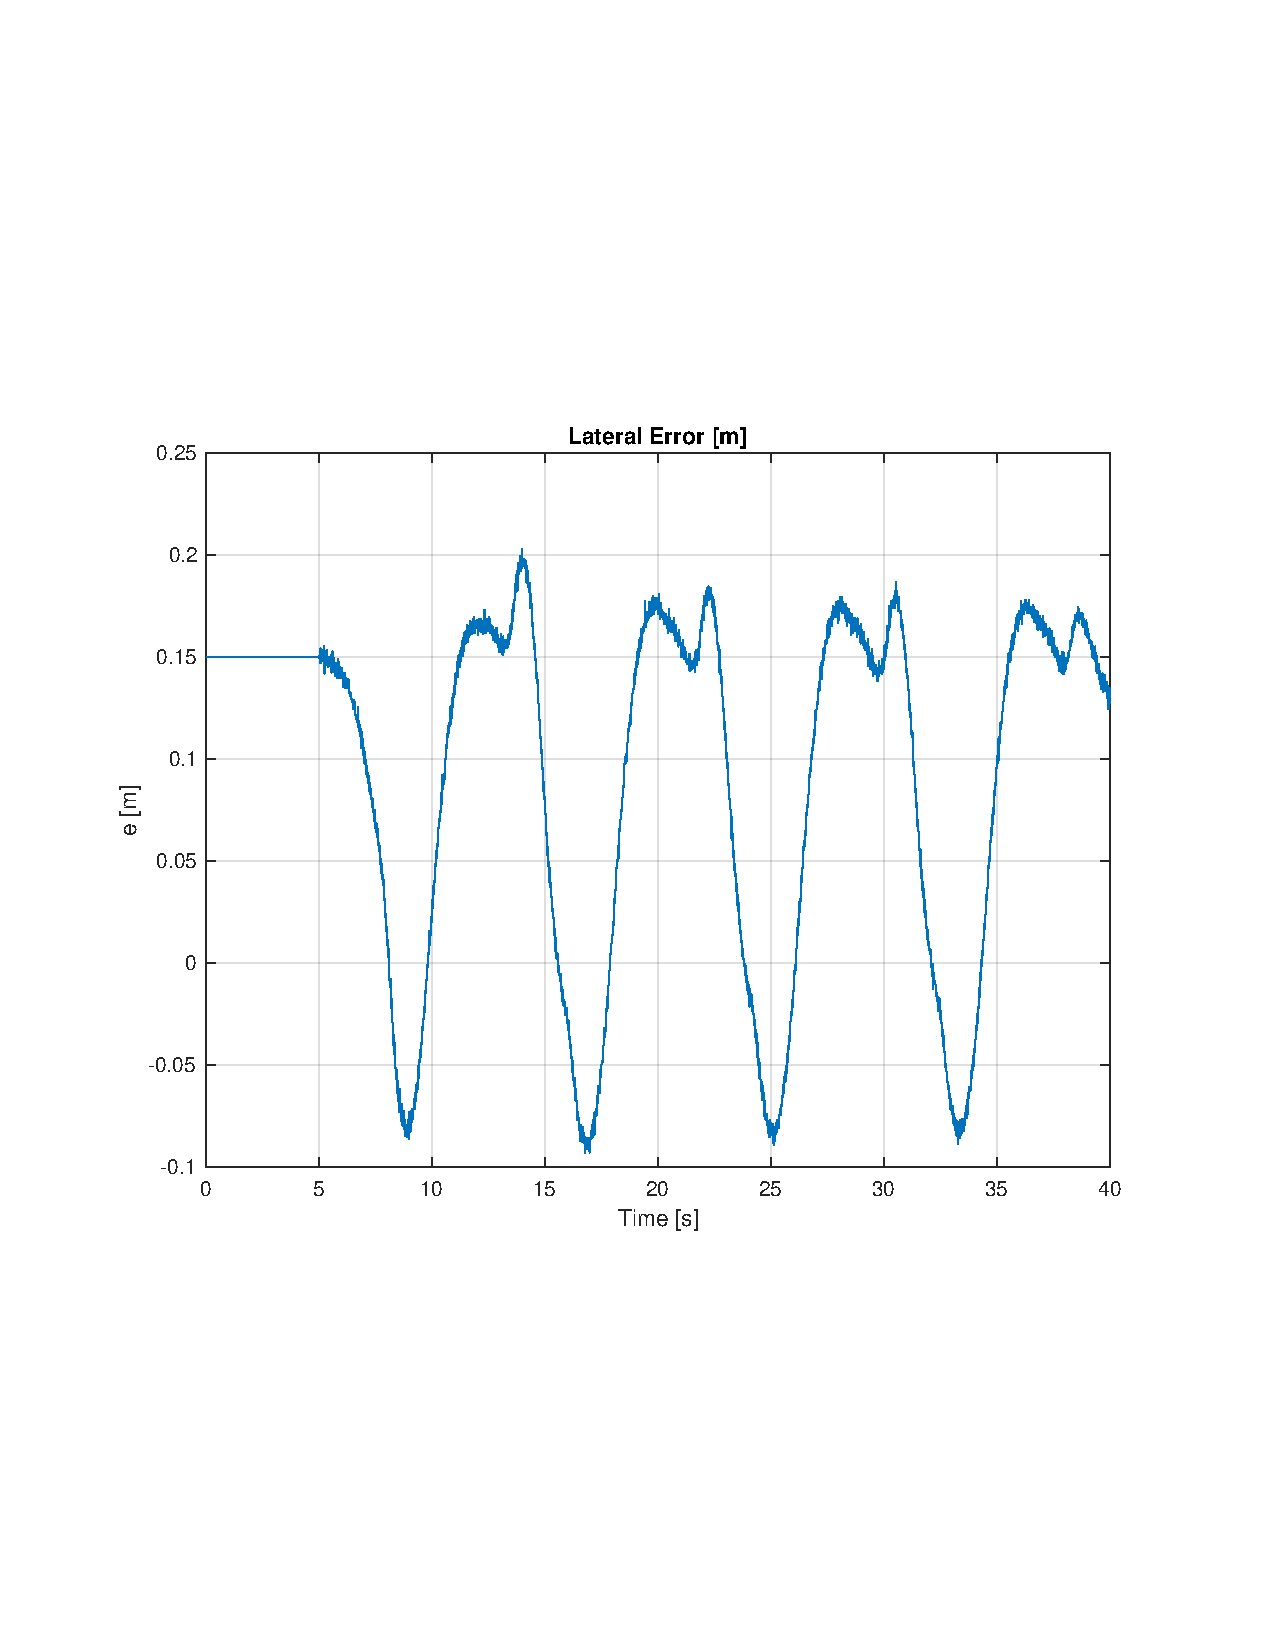
\includegraphics[width =0.6\textwidth]{e_Profile.pdf}
        \vspace{-7.5mm}
        \caption{Simulation of optimal design point $x^*$ for lateral error vs time}
        \label{fig:e-profile}
    \end{center}
\end{figure}

\begin{figure}[H]
    \begin{center}
        \vspace{-2.5mm}
        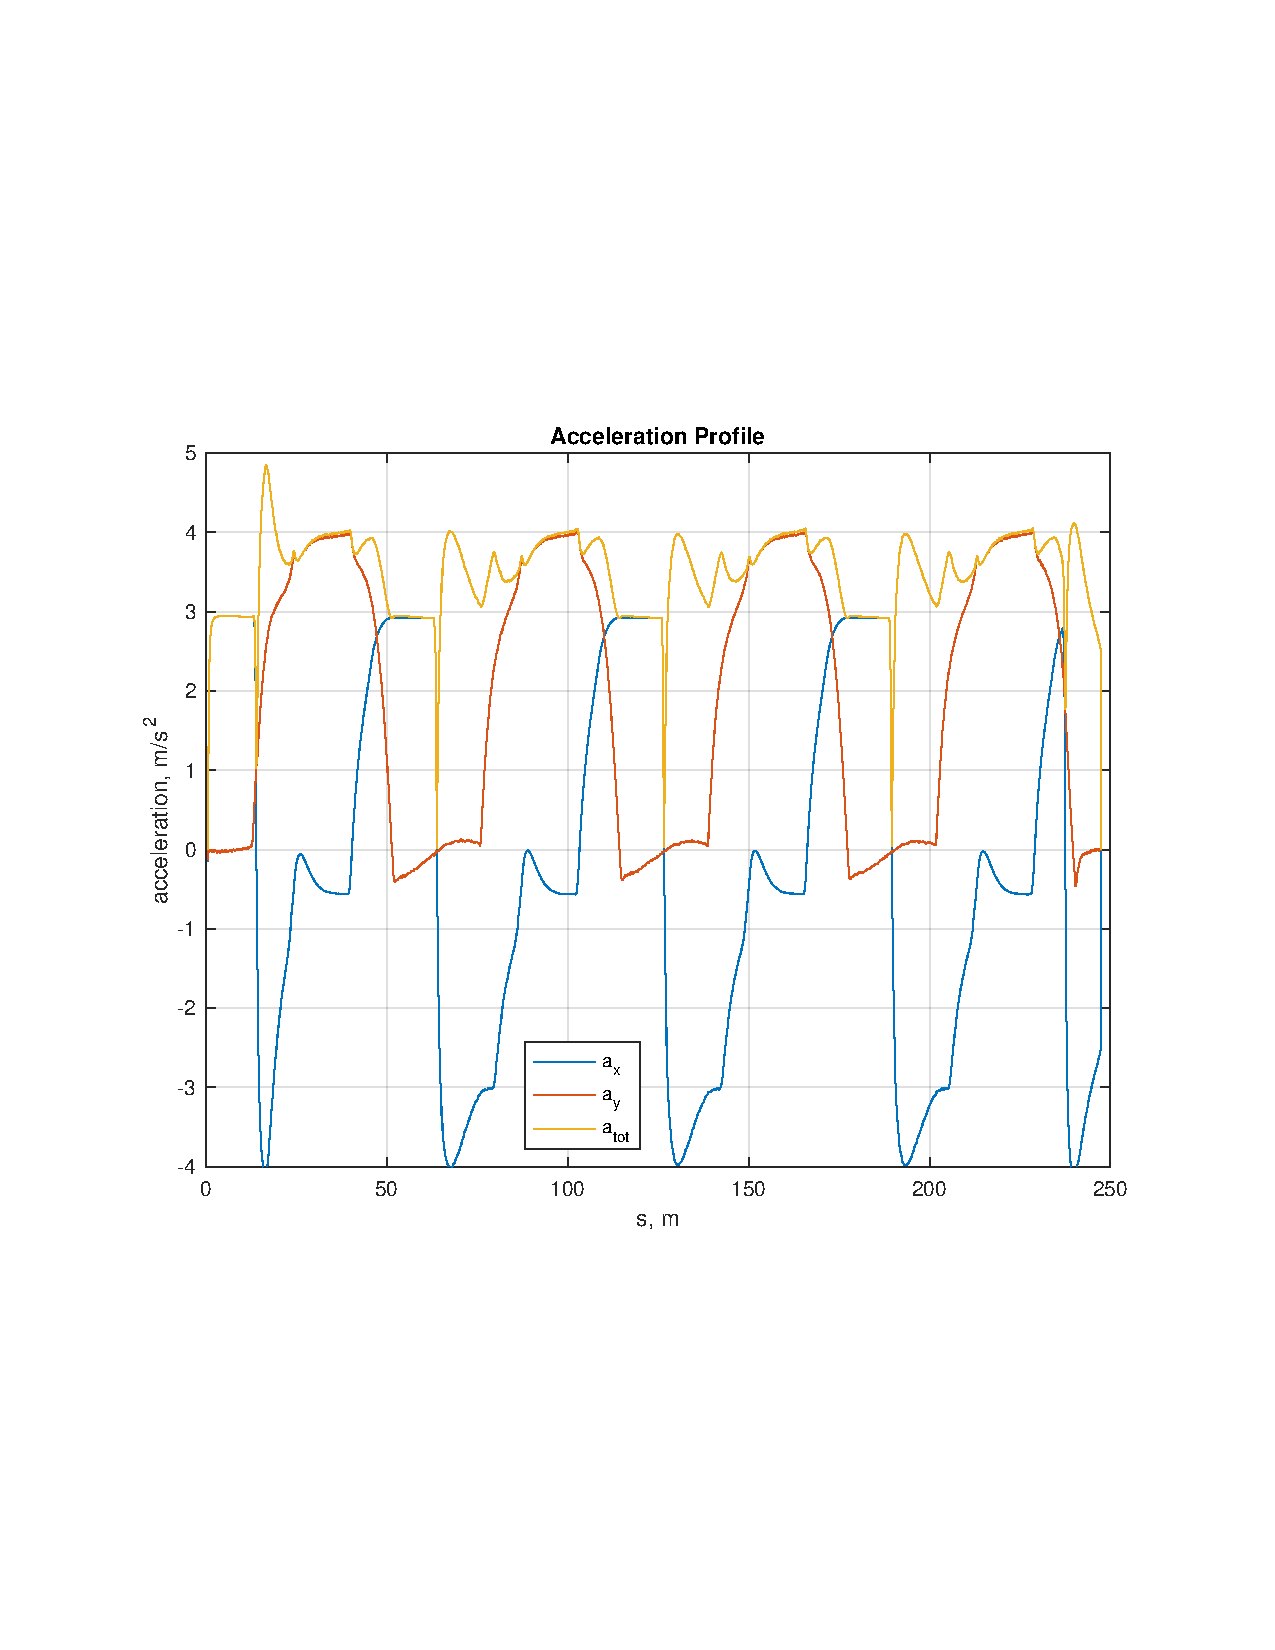
\includegraphics[width =0.6\textwidth]{Acceleration_Profiles.pdf}
        \vspace{-7.5mm}
        \caption{Simulation of optimal design point $x^*$ for longitudinal and lateral accelerations vs time}
        \label{fig:acc-profile}
    \end{center}
\end{figure}

The simulation results in figure 7 above show that the lateral error profile fell nearly perfectly within the set constraint, only to slightly exceed the constraint value of 0.2 m at around 14 seconds.

\subsection{Optimal design point simulation results}

\section{Conclusion}


\section*{Appendix}


\section*{Acknowledgments}


\bibliography{sample}

\end{document}
